%%----------------------------------------------------------------------------------------
%	PACKAGES AND THEMES
%----------------------------------------------------------------------------------------
\PassOptionsToPackage{table}{xcolor}
\documentclass[aspectratio=169,xcolor=dvipsnames,svgnames,x11names,fleqn]{beamer}
% \documentclass[aspectratio=169,xcolor=dvipsnames,fleqn]{beamer}

\usetheme{RedVelvet}

\usefonttheme[onlymath]{serif}
\newcommand{\showanswers}{yes}
\usepackage{pifont} % For checkmarks and crosses

\usepackage{setspace}
\usepackage{xspace}
\usepackage{amsmath}
\usepackage{amssymb}
\usepackage{amsfonts}
\usepackage{color}
\usepackage{physics}
% \usepackage{mathbb}
\usepackage{rahul_math}
\usepackage{bigints}

\usepackage[utf8]{inputenc}
\usepackage[ruled,vlined]{algorithm2e}
\usepackage{amsmath}
\usepackage{amsfonts}

\usepackage{graphicx} % Allows including images
\usepackage{booktabs} % Allows the use of \toprule, \midrule and \bottomrule in tables
\usepackage{tikz,pgfplots}
\usepackage{mathtools}
\usepackage{subfigure}
\usetikzlibrary{arrows}
\usepackage{minted}
\definecolor{LightGray}{gray}{0.9}
\definecolor{cream}{rgb}{0.92, 0.9, 0.55}
\definecolor{lightblue}{rgb}{0.68, 0.85, 0.9}


\usepackage{xcolor-material}
\usetikzlibrary{fit}
\usetikzlibrary{matrix}
\tikzset{%
apple/.pic={
    \fill [MaterialBrown] (-1/8,0)  arc (180:120:1 and 3/2) coordinate [pos=3/5] (@)-- ++(1/6,-1/7)  arc (120:180:5/4 and 3/2) -- cycle;
    \fill [MaterialLightGreen500] (0,-9/10)  .. controls ++(180:1/8) and ++(  0:1/4) .. (-1/3,  -1) .. controls ++(180:1/3) and ++(270:1/2) .. (  -1,   0) .. controls ++( 90:1/3) and ++(180:1/3) .. (-1/2, 3/4) .. controls ++(  0:1/8) and ++(135:1/8) .. (   0, 4/7)
    }
    }

\newcommand{\leftdoublequote}{\textcolor{blue}{\scalebox{3}{``}}}

\newcommand{\rightdoublequote}{\textcolor{blue}{\scalebox{3}{''}}}


\usepackage{textcomp}
\usepackage{fontawesome}
\usepackage{tikz,pgfplots}
\usetikzlibrary{shapes.callouts}
\usetikzlibrary{arrows}
\usetikzlibrary{shapes.geometric, positioning}
\usetikzlibrary{matrix,positioning,decorations.pathreplacing,calc}
\usepackage{tikz-dependency}

\pgfplotsset{compat=1.8} % or newest version

\usetikzlibrary{positioning}


\usepackage{bm}
\usepackage{relsize}

\tcbuselibrary{skins, hooks}

\tikzset{basic/.style={draw,fill=MediumBlue!20,text width=1em,text badly centered}}
\tikzset{input/.style={basic,circle}}
\tikzset{weights/.style={basic,rectangle}}
\tikzset{functions/.style={basic,circle,fill=MediumBlue!10}}



\usepackage{listofitems} % for \readlist to create arrays
\tikzstyle{mynode}=[thick,draw=MediumBlue,fill=MediumBlue!20,circle,minimum size=22]


\usepackage{overpic}

%----------------------------------------------------------------------------------------
%	TITLE PAGE
%----------------------------------------------------------------------------------------

\usepackage{tikz-qtree,tikz-qtree-compat}
\usetikzlibrary{tikzmark}
\usetikzlibrary{calc}

\usetikzlibrary{fit}
\tikzset{%
apple/.pic={
    \fill [MaterialBrown] (-1/8,0)  arc (180:120:1 and 3/2) coordinate [pos=3/5] (@)-- ++(1/6,-1/7)  arc (120:180:5/4 and 3/2) -- cycle;
    \fill [MaterialLightGreen500] (0,-9/10)  .. controls ++(180:1/8) and ++(  0:1/4) .. (-1/3,  -1) .. controls ++(180:1/3) and ++(270:1/2) .. (  -1,   0) .. controls ++( 90:1/3) and ++(180:1/3) .. (-1/2, 3/4) .. controls ++(  0:1/8) and ++(135:1/8) .. (   0, 4/7)
}
}
\usepackage{tikz-qtree,tikz-qtree-compat}
\usetikzlibrary{tikzmark}
\usetikzlibrary{calc}

\usetikzlibrary{positioning}
\newcommand{\vect}[1]{\mathbf{#1}}
% Define styles
\tikzset{
    box/.style={
        rectangle,
        draw=black,
        fill=blue!20,
        text width=2.2cm,
        text centered,
        minimum height=0.8cm,
        font=\small
    },
    arrow/.style={
        ->,
        >=Stealth,
        line width=1.5pt,
        draw=black
    }
}


\usepackage{bm}
\usepackage{relsize}



\tikzset{basic/.style={draw,fill=MediumBlue!20,text width=1em,text badly centered}}
\tikzset{input/.style={basic,circle}}
\tikzset{weights/.style={basic,rectangle}}
\tikzset{functions/.style={basic,circle,fill=MediumBlue!10}}
\usetikzlibrary{arrows.meta, bending}
\usetikzlibrary{shapes.geometric, arrows.meta, positioning, fit, backgrounds}

\usepackage{listofitems} % for \readlist to create arrays
\tikzstyle{mynode}=[thick,draw=MediumBlue,fill=MediumBlue!20,circle,minimum size=22]


\newmdenv[
backgroundcolor=androidYellowLight,
linecolor=androidYellow,
linewidth=0.5pt,
roundcorner=10pt,
skipabove=\baselineskip,
skipbelow=\baselineskip
]{MintedFrame}

% Set minted options
\setminted{
fontsize=\footnotesize,
breaklines=true,
autogobble,
linenos,
frame=none
}


\title[CPE 487/587: Deep Learning]{CPE 486/586: Deep Learning for Engineering Applications} % The short title appears at the bottom of every slide, the full title is only on the title page
\subtitle{09 Reinforcement Learning}

\author[Rahul Bhadani] {{\Large \textbf{Rahul Bhadani}}}

\institute[UAH] % Your institution as it will appear on the bottom of every slide, maybe shorthand to save space
{
    Electrical \& Computer Engineering,  The University of Alabama in Huntsville
}
\date

% \titlegraphic{
%    \includegraphics[width=0.4\linewidth]{figures/UAH_primary.png}
% }

\begin{document}

%-------------------------------------------------
\begin{frame}
    \titlepage
\end{frame}

%-------------------------------------------------
\begin{frame}{Outline}
    \backgroundtableofcontents
\end{frame}

%------------------------------------------------
\section{Motivation}
%------------------------------------------------

\begin{frame}{}
    \begin{center}
    \huge \bf \color{DarkBlue}
    Motivation:

    Learning in Dynamic Environments

        
\includegraphics[width=0.29\textwidth]{figures/human_robot.png}
        
\end{center}

\end{frame}


%------------------------------------------------

\begin{frame}
\frametitle{Dynamic Environments}

\begin{columns}[c] % The "c" option specifies centered vertical alignment while the "t" option is used for top vertical alignment

    \column{.45\textwidth} % First column and width
    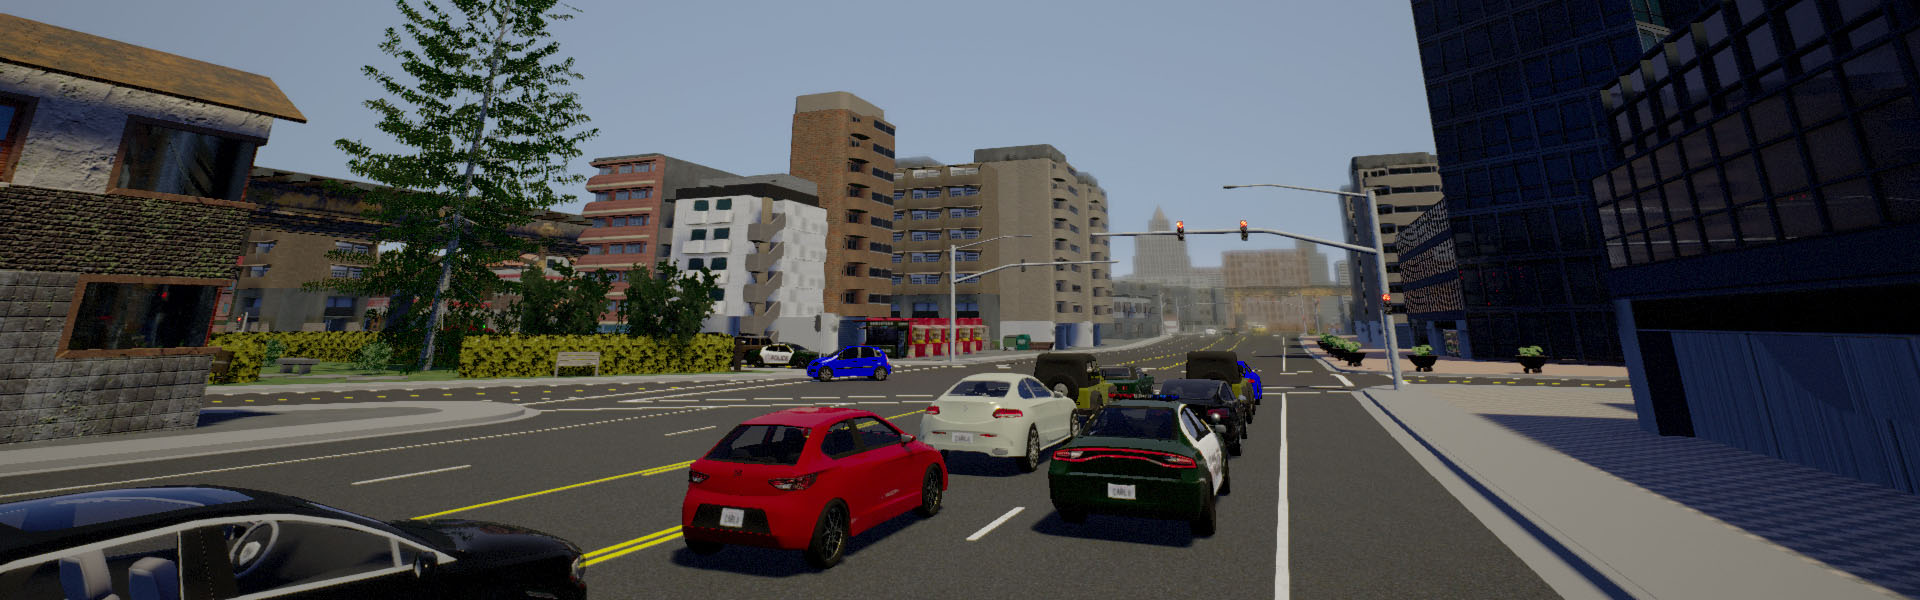
\includegraphics[width=\textwidth]{figures/carla.jpg}

    \column{.45\textwidth} % Second column and width
    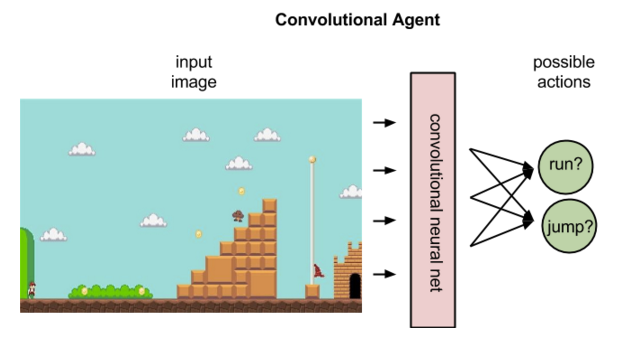
\includegraphics[width=0.9\textwidth]{figures/supermario.png}

\end{columns}

\begin{columns}[c] % The "c" option specifies centered vertical alignment while the "t" option is used for top vertical alignment

    \column{.20\textwidth} % Third column and width
    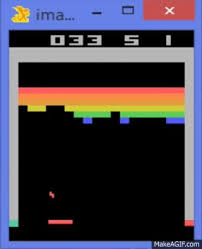
\includegraphics[width=\textwidth]{figures/atari.jpeg}

    \column{.20\textwidth} % Fourth column and width
    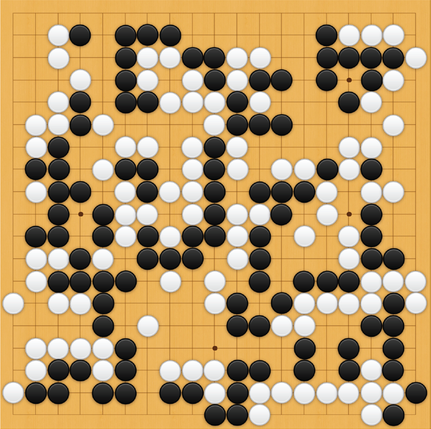
\includegraphics[width=\textwidth]{figures/alphago.png}

\end{columns}

\end{frame}

%------------------------------------------------


\begin{frame}{Reinforcement Learning in Robotics}

\begin{center}
        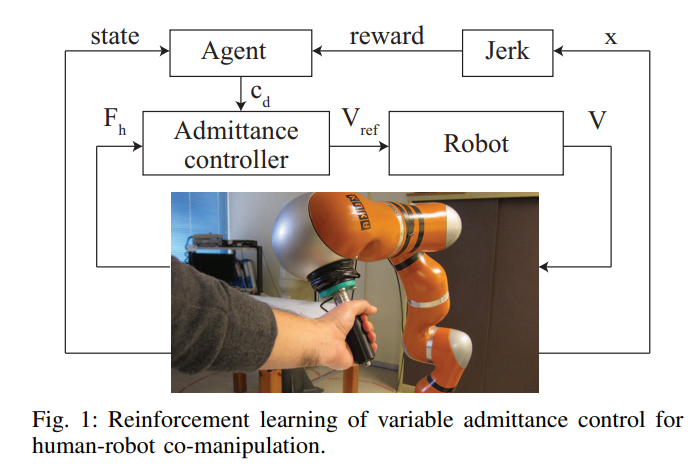
\includegraphics[width=0.5\textwidth]{figures/rl_robotics.png}

        Dimeas, Fotios, and Nikos Aspragathos. "Reinforcement learning of variable admittance control for human-robot co-manipulation." 2015 IEEE/RSJ International Conference on Intelligent Robots and Systems (IROS). IEEE, 2015.
\end{center}

\end{frame}

%------------------------------------------------


\begin{frame}{Reinforcement Learning in Games}

\begin{center}
        Super Mario: \url{https://youtu.be/OQitI066aI0}

        Starcraft: \url{https://youtu.be/gEyBzcPU5-w}
\end{center}

\end{frame}

%------------------------------------------------

\begin{frame}{Class of Learning Problems}

    \small

    \begin{columns}[c] % The "c" option specifies centered vertical alignment while the "t" option is used for top vertical alignment

    \column{.33\textwidth} % Third column and width
    \textbf{Supervised Learning:}
    \begin{itemize}
        \item Given training data with previously labeled classes, learn the
mapping between the data and their correct classes
\item Data: $(\xbf, \ybf)$
\item Goal: learning mapping $\xbf \to \ybf$.
\item This is a leaf: {\Huge \textleaf}

    \end{itemize}

    \column{.33\textwidth} % Third column and width
    \textbf{Unsupervised Learning:}
    \begin{itemize}
        \item Given unlabeled data, learn how to group such data into meaningful clusters based on some measure of similarity
\item Data: $\xbf$
\item Goal: learn the underlying structure
\item These two are similar: {\huge \textleaf}, {\huge \faLeaf}

    \end{itemize}

    \column{.33\textwidth} % Third column and width
    \textbf{Reinforcement Learning:} 
    \begin{itemize}
    \item Given a sequence of outputs, learn a policy to obtain the desired output 
    \item Data: state-action pairs
    \item Goal: maximize future rewards over many time-steps
    \item Eat this to stay alive: {\Huge \faLeaf}

\end{itemize}

\end{columns}

    
\end{frame}

%------------------------------------------------

\section{Reinforcement Learning}


\begin{frame}{}
    \begin{center}
    \huge \bf \color{DarkBlue}
    Reinforcement Learning
\end{center}

\end{frame}

%------------------------------------------------


\begin{frame}{Reinforcement Learning: A High-level Picture}
\begin{center}
        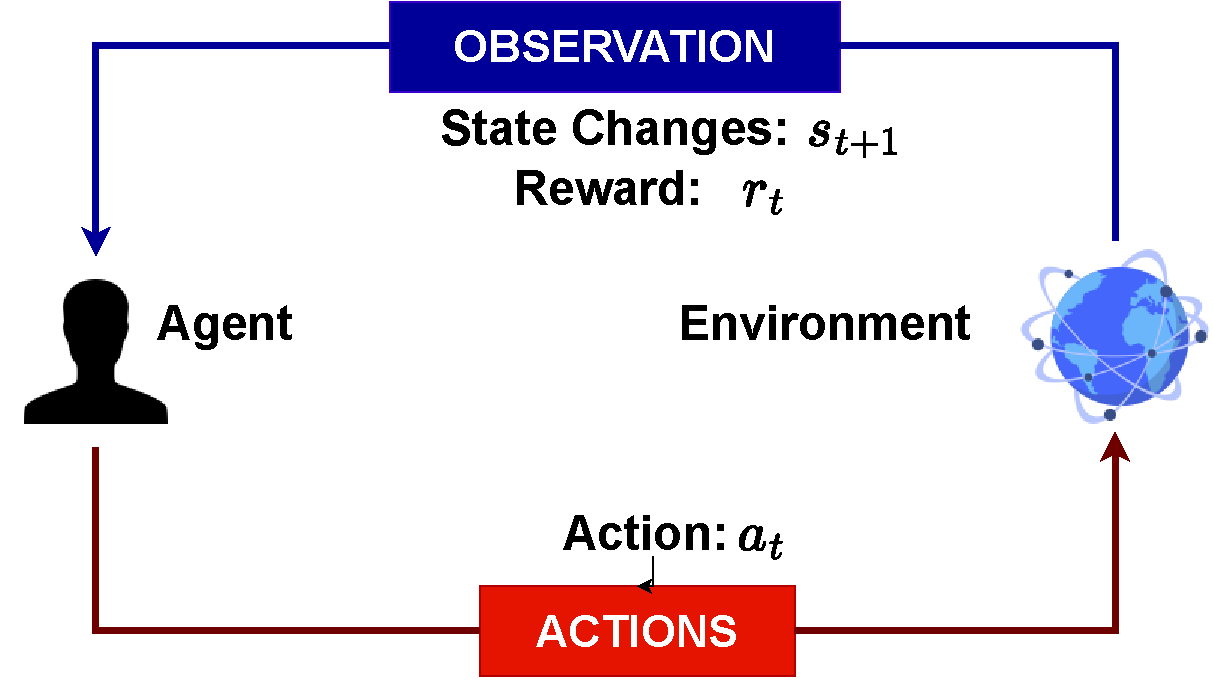
\includegraphics[width=0.75\textwidth]{figures/RL_diagram.pdf}
\end{center}
    
\end{frame}

%------------------------------------------------


\begin{frame}{Reinforcement Learning (RL): Cart-pole Problem}
\begin{center}
\begin{columns}[c] % The "c" option specifies centered vertical alignment while the "t" option is used for top vertical alignment

    \column{.40\textwidth} 
    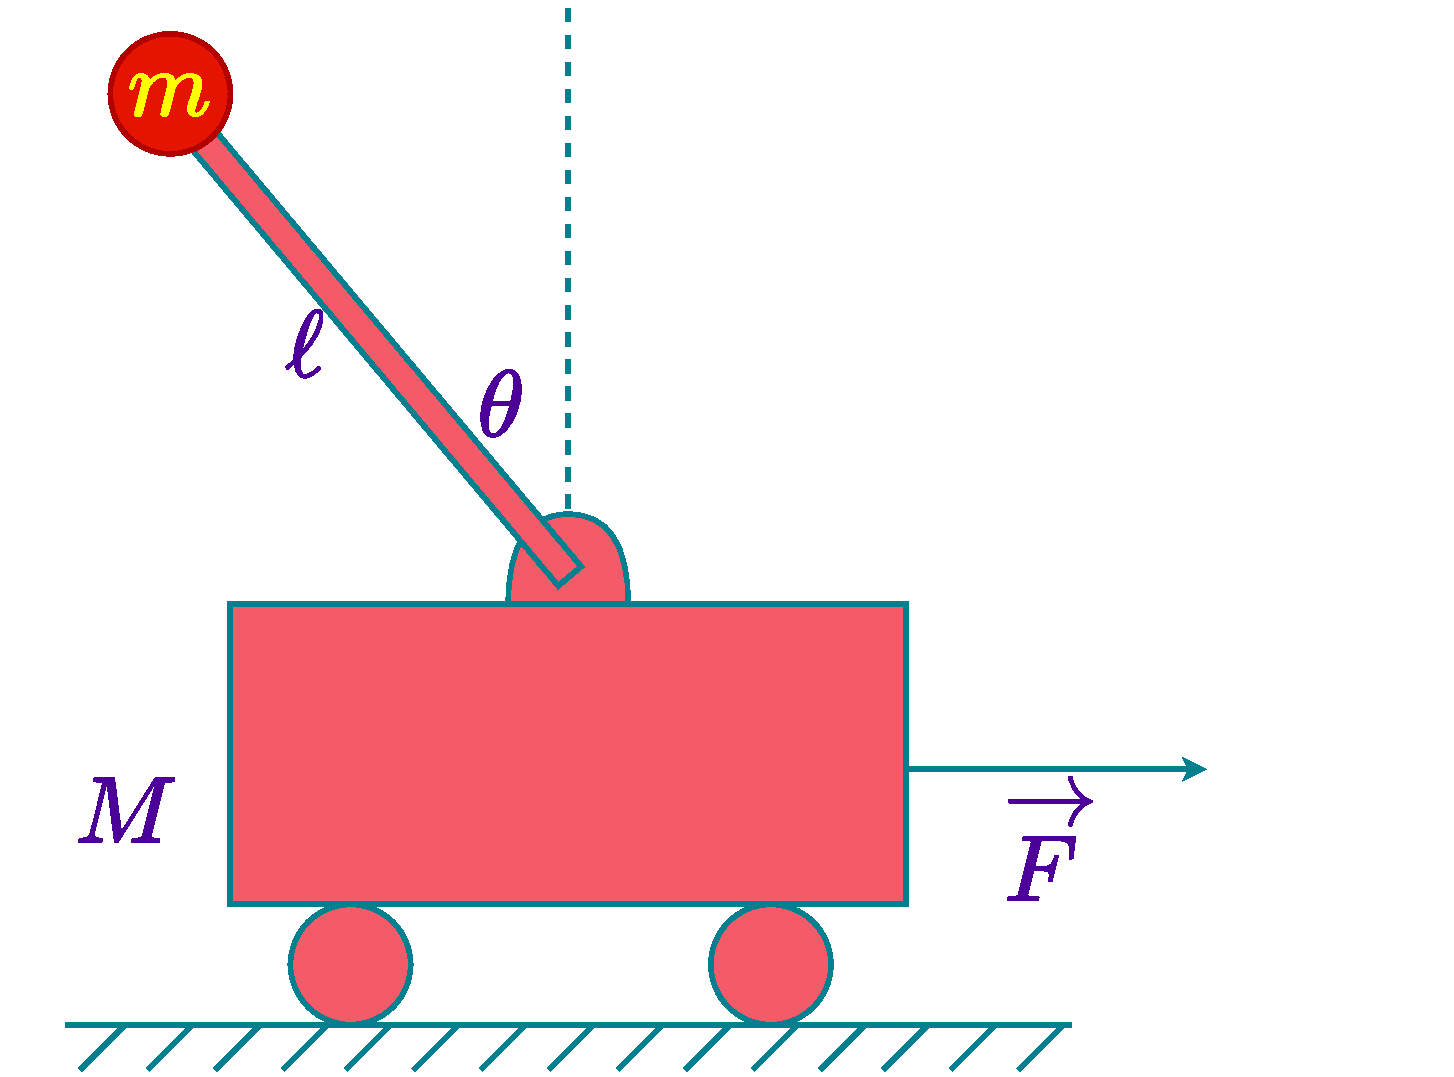
\includegraphics[width=0.99\textwidth]{figures/carpole.pdf}

    \column{.60\textwidth} 

\textbf{Objective:} Balance a pole on the top of a wheeled cart.

\textbf{State:} angle, angular speed, position, horizontal velocity.

\textbf{Action:} horizontal force applied to the car.

    \textbf{Reward:} $+10$ at each time step if the pole is upright.
    
    \end{columns}

\end{center}
    
\end{frame}


%------------------------------------------------


\begin{frame}{RL: Key Concepts}

\begin{columns}[c] % The "c" option specifies centered vertical alignment while the "t" option is used for top vertical alignment

    \column{.70\textwidth} 
    
    \begin{tblock}{\textbf{Agent}}
    that takes actions in the environment and interacts with it and other agents.

    \end{tblock}

    \column{.30\textwidth} 
    {\Huge\faAndroid~~\faMale~~\faUsers~~\faCar }

    \end{columns}

        \begin{columns}[c] % The "c" option specifies centered vertical alignment while the "t" option is used for top vertical alignment

    \column{.70\textwidth} 
    
    \begin{peach}{\textbf{Environment}}
the world in which the agent (or agents) operate(s).

    \end{peach}

    \column{.30\textwidth} 
    {\Huge\faGlobe}

        \end{columns}
        
\end{frame}



%------------------------------------------------
\begin{frame}{RL: Key Concepts}

\begin{columns}[c] % The "c" option specifies centered vertical alignment while the "t" option is used for top vertical alignment

    \column{.70\textwidth} 
    
    \begin{tblock}{\textbf{Action} $a_t$}
A move that an agent can make in the environment. Can be continuous (steering angle in car driving) or discrete (chess moves).
    \end{tblock}

    \column{.30\textwidth} 
    {\Huge \faArrowDown~~\faArrowUp~~\faArrowLeft~~\faArrowRight }

    \end{columns}

\end{frame}

%------------------------------------------------
\begin{frame}{RL: Key Concepts}

\begin{columns}[c] % The "c" option specifies centered vertical alignment while the "t" option is used for top vertical alignment

    \column{.70\textwidth} 
    
    \begin{tblock}{\textbf{State} $s_t$}
A situation that an agent perceives or is in. 

Example: current speed of a car, its GPS location: latitude, longitude, acceleration.
    \end{tblock}

    \column{.30\textwidth} 
    {\Huge \faChartLine~~\faLocationArrow}

\end{columns}

\end{frame}
%------------------------------------------------
\begin{frame}{RL: Key Concepts}

\begin{columns}[c] % The "c" option specifies centered vertical alignment while the "t" option is used for top vertical alignment

    \column{.80\textwidth} 
    
    \begin{tblock}{\textbf{Reward} $r_t$}
A feedback by which we measure the success or failure of the agent's action.

Example: Mario jumping to collect coins results in an increased point or gain of an additional lifeline.

\textbf{Note:} Not all actions may result in an immediate reward. It may also be in a delayed fashion.
    \end{tblock}

    \column{.20\textwidth} 
    {\huge \faMoneyBill~~\faBitcoin~~\faDollarSign}

\end{columns}
\vspace{10pt}
\textbf{ Total reward/return} $R_t = \sum_{i=t}^\infty r_i = r_t+ r_{t+1} + \cdots + r_{t+n}$.

\vspace{10pt}
\textbf{ Discounted reward} $R_t = \sum_{i=t}^\infty \gamma^i r_i $. This makes future rewards less appealing than the current reward (but also makes infinite sum convergent).

\end{frame}
%------------------------------------------------


\begin{frame}{Markov Property}

    \begin{center}
        \large
    \leftdoublequote    Markov property: All future states depend on the current state only. \rightdoublequote

    \vspace{1em}

    In other words, the current state completely characterizes the state of the world.
    \end{center}
\end{frame}


\begin{frame}{Markov Property}
    \begin{tblock}{Basic Markov Chain}
        A standard Markov chain is defined by:
        \begin{itemize}
            \item A set of states $S = \{s_1, s_2, \ldots, s_n\}$
            \item A transition matrix $P$ where $P_{ij}$ is the probability of transitioning from state $i$ to state $j$
        \end{itemize}
    \end{tblock}
        
        \begin{tblock}{}
            \small
        The key property is the Markov property:
        \begin{multiequation}
            P(X_{t+1} = s_j | X_t = s_i, X_{t-1} = s_{i-1}, \ldots, X_0 = s_{i_0}) = P(X_{t+1} = s_j | X_t = s_i) = P_{ij}
        \end{multiequation}
        \end{tblock}
\end{frame}

%------------------------------------------------

\begin{frame}{Markov Process/Markov Chain}
\begin{talert}{Definition}
A finite state machine where each state is a Markov state (i.e. follows the Markov property).

It consists of a number of states with transition probabilities from one state to another.
\end{talert}

\begin{center}
    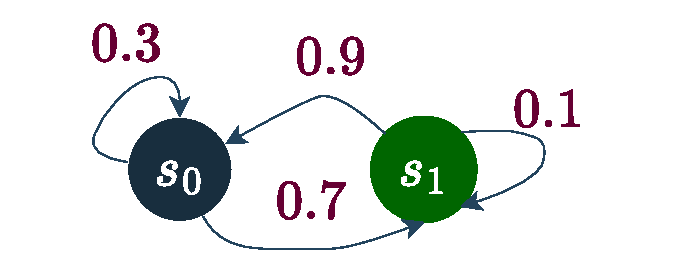
\includegraphics[width=0.55\textwidth]{figures/MarkovChain.pdf}
\end{center}

\footnotesize Reading: Introduction to Probability Models by Sheldon M. Ross, Chapter 4.

\end{frame}

\begin{frame}{Steady State Distribution Calculation for a Markov Chain}

    \begin{tblock}{Steady State Distribution}
        The \textbf{steady-state probabilities} (or equilibrium probabilities) of a Markov chain refer to a set of probabilities that remain constant over time, under the condition that the system evolves for a sufficiently long time. These probabilities indicate the proportion of time the process spends in each state in the long run.
    \end{tblock}
\end{frame}

\begin{frame}{Steady State Distribution Calculation for a Markov Chain}

    Let $\Omega$ be the vector of steady-state probabilities, then   satisfies the following equation:

    \begin{multiequation}
        \Omega P & = \Omega\\
        \Omega(P - I) & = 0\\
        (P^\top - I)\Omega^\top  & = 0 \quad \text{(Writing in the form $Ax = b$)}
    \end{multiequation}
where $P$ is the transition matrix. It can be solved using the linear algebra solvers. Alternative it is also an Eigenvalue problem and can be solved using standard libraries for Eignevalues.

\end{frame}
%------------------------------------------------

\begin{frame}{}
    \Large
    \begin{center}
        Now add actions to the state transition.
    \end{center}

    \begin{center}
        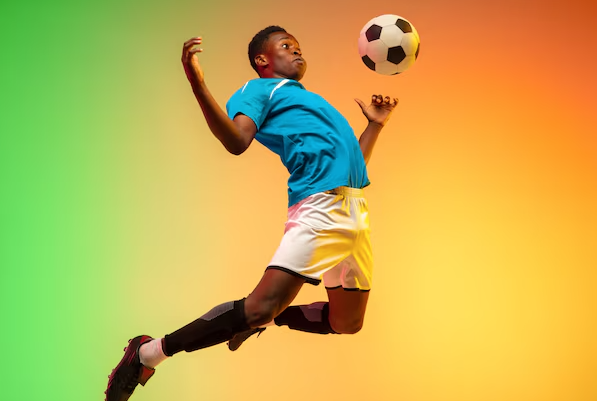
\includegraphics[width=0.45\textwidth]{figures/soccer_action.png}
\end{center}

\end{frame}


\begin{frame}{Markov Decision Process (MDP)}

\large

    \begin{tblock}{}
        An extension of Markov chain with state transition depending on some action $a$. 
    \end{tblock}

\end{frame}
%------------------------------------------------

\begin{frame}{Adding Actions to Markov Chains}
    \begin{tblock}{}
        When we add actions, we extend the formulation to:
        \begin{itemize}
            \item A set of states $S = \{s_1, s_2, \ldots, s_n\}$
            \item A set of actions $A = \{a_1, a_2, \ldots, a_m\}$
            \item A set of transition matrices $\{P^a\}_{a \in A}$ where $P^a_{ij}$ is the probability of transitioning from state $i$ to state $j$ when taking action $a$
        \end{itemize}
        \end{tblock}
        
        \begin{tblock}{}
        \begin{multiequation}
            P(X_{t+1} = s_j | X_t = s_i, A_t = a) = P^a_{ij}
        \end{multiequation}
        Where $A_t$ is the action taken at time $t$.
        \end{tblock}
\end{frame}

\begin{frame}{}
    \begin{center}
        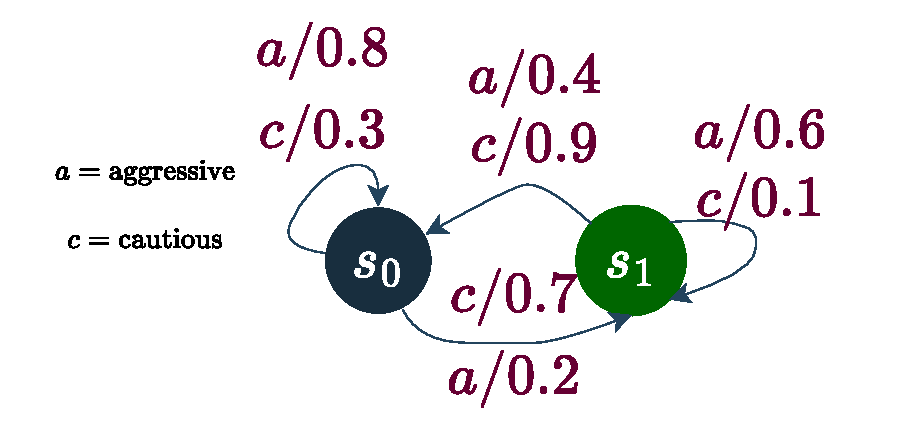
\includegraphics[width=0.85\textwidth]{figures/MarkovChain_WithActions.pdf}
    \end{center}
    
\end{frame}


\begin{frame}{State Sequences}
    \begin{tblock}{}
        When generating a sequence of states based on actions, we iteratively apply:
        \begin{multiequation}
            X_{t+1} \sim P^{A_t}_{X_t}
        \end{multiequation}
        Where $\sim$ indicates sampling from the probability distribution in row $X_t$ of transition matrix $P^{A_t}$.
        \end{tblock}
        
        \begin{tblock}{}
        For each time step $t$:
        \begin{enumerate}
            \item Choose action $A_t$ (predefined or by some policy)
            \item Sample next state $X_{t+1}$ from the probability distribution $P^{A_t}_{X_t, \cdot}$
            \item Update current state $X_t \leftarrow X_{t+1}$
        \end{enumerate}
        \end{tblock}
\end{frame}

\begin{frame}{}
    \Large
    \begin{center}
        Now add rewards to the Markov Decision Processes favoring certain actions over another.
    \end{center}

    \begin{center}
        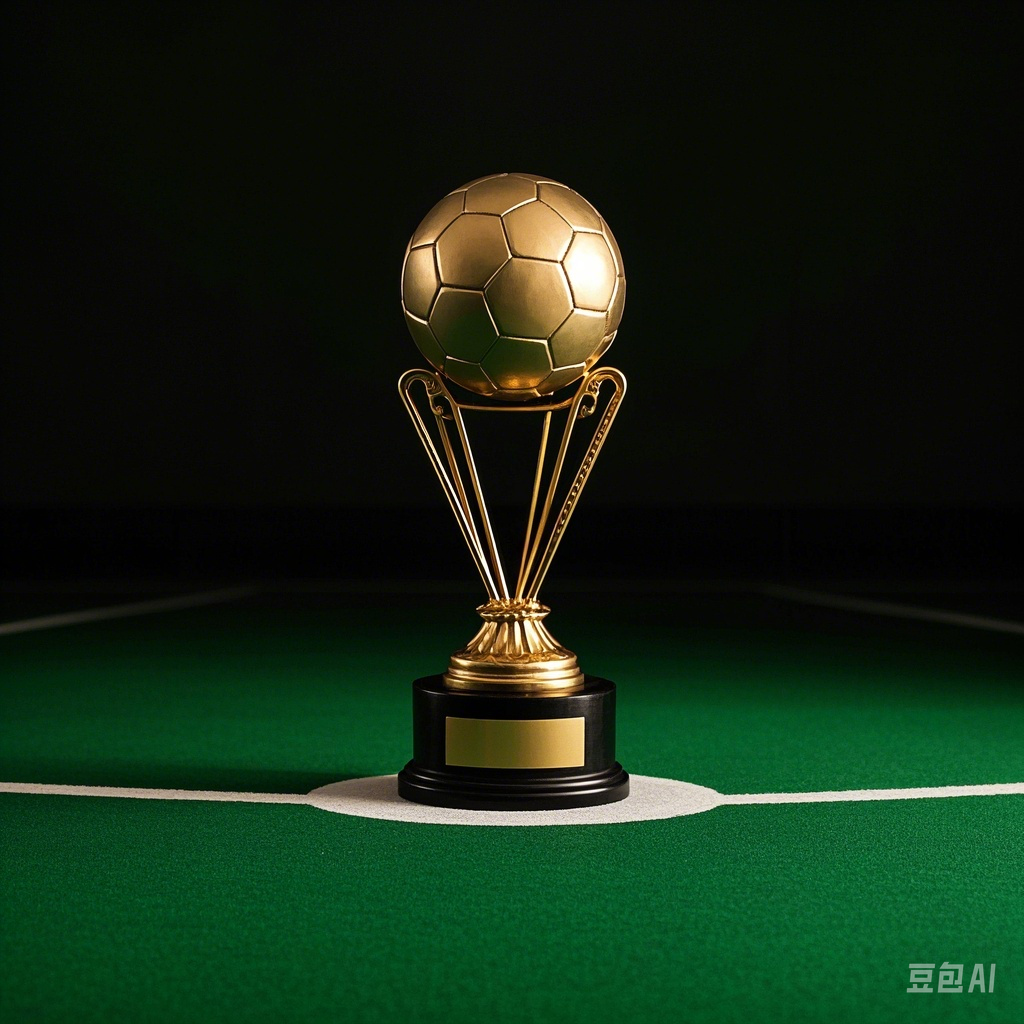
\includegraphics[width=0.45\textwidth]{figures/soccer_reward.png}
\end{center}

\end{frame}


\begin{frame}{}
    \begin{center}
        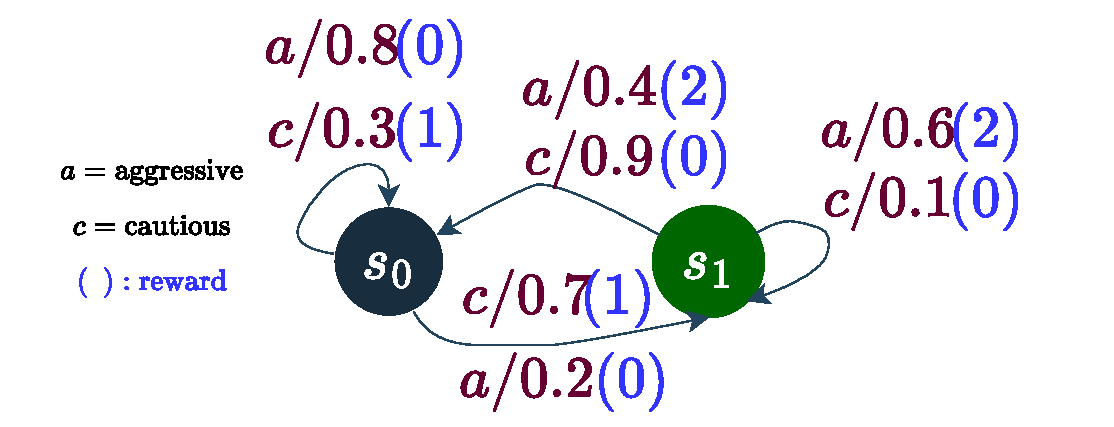
\includegraphics[width=0.85\textwidth]{figures/MarkovChain_WithActionsAndReward.pdf}
    \end{center}
    
\end{frame}

\begin{frame}{Markov Decision Process (MDP)}

\begin{itemize}
    \item The transition leads to some corresponding reward.
    \item An MDP in the context of reinforcement learning is a 5-tuple model $(\Scal, \Acal, \Pcal, \Rcal, \gamma)$ where 
\begin{itemize}
    \item \textcolor{red}{$\Scal:$ set of  possible states, $s\in \Scal$ is a state.}
    \item \textcolor{blue}{$\Acal:$ set of possible actions taken while an agent is in a state $s$, $a\in\Acal$ is an action.}
    \item \textcolor{red}{$\Pcal:$ a transition probability matrix for defining probabilities of transition to a state $s'$ from a state $s$ under the influence of action $a$ or some other conditional probability density function; written as $\Pcal(s'|s, a)$.}
    \item \textcolor{blue}{$\Rcal:$ Distribution of reward given state action pair; a reward $r(s, a) \in \Rcal$ is reward for moving to state $s$ under action $a$.}
    \item \textcolor{red}{$\gamma:$ discount factor, used to emphasize short-term reward over long-term reward; a mathematical trick to make infinite sum finite.}
\end{itemize}
    
\end{itemize}
    
\end{frame}

%------------------------------------------------
\begin{frame}{Markov Decision Process}
A time step $t=0$, the environment samples the initial state $s_0 \sim p(s_0)$ (stochastic condition).

For $t = 0$ until done: 
\begin{itemize}
    \item Agent picks an action $a_t$
    \item Environment calculates the probable reward $r_t\sim  \Rcal(~\cdot~ | s_t, a_t)$
    \item Environment samples the next state $s_{t+1}\sim P(~\cdot~ | s_t, a_t)$
    \item Agent receives the reward $r_t$ and the next state $s_{t+1}$
    \item Increment $t$.
\end{itemize}

\footnotesize
\begin{center}
    Reading: Ma, H., Han, S., Hemida, A., Kamhoua, C., \& Fu, J. \textbf{Adaptive Incentive Design for Markov Decision Processes with Unknown Rewards}. \url{https://openreview.net/pdf?id=Rwf31BYTAU}
\end{center}
    
\end{frame}

\begin{frame}{Different Types of Rewards}

    \begin{itemize}
        \item State-Action Reward $r(s,a)$: reward depends only on the current state and action;
        \item State-Action-State Reward $r(s, a, s')$: reward depends on the current state, action and the result state;
        \item  State-only Reward $r(s)$:  reward depends only on the state you are in.
    \end{itemize}
    
\end{frame}


%------------------------------------------------

\begin{frame}{Policy Function}
The policy function, usually denoted by $\pi$ in the RL literature specifies the mapping from state space $\Scal$ to Action space $\Acal$.
\vspace{10pt}
It tells, what action to perform in each state.
\vspace{10pt}
We denote the policy function as $\pi(s): \Scal \to \Acal$. 
\vspace{10pt}
Our ultimate goal in the RL scenario lies in finding the optimal policy that specifies the correct action to perform in each state, which maximizes the reward.

\end{frame}


%------------------------------------------------

\begin{frame}{Episodic and Continuous Tasks}

\begin{peach}{Episodic Tasks}
    Episodic tasks are the tasks that have a terminal state (end). For example, in a car racing game, the end of the game is a terminal state. Once the game is over, you start the next episode by restarting the game which will be a whole new beginning. 
\end{peach}

\begin{gradblock}{Continuous Tasks}
    In continuous tasks, there is no terminal state. For example, a robot navigating in a warehouse is a continuous task and there is no defined endpoint as long as operations are required.
\end{gradblock}

\end{frame}




%------------------------------------------------

\begin{frame}{Example MDP through State Diagram}
    
    \begin{center}
        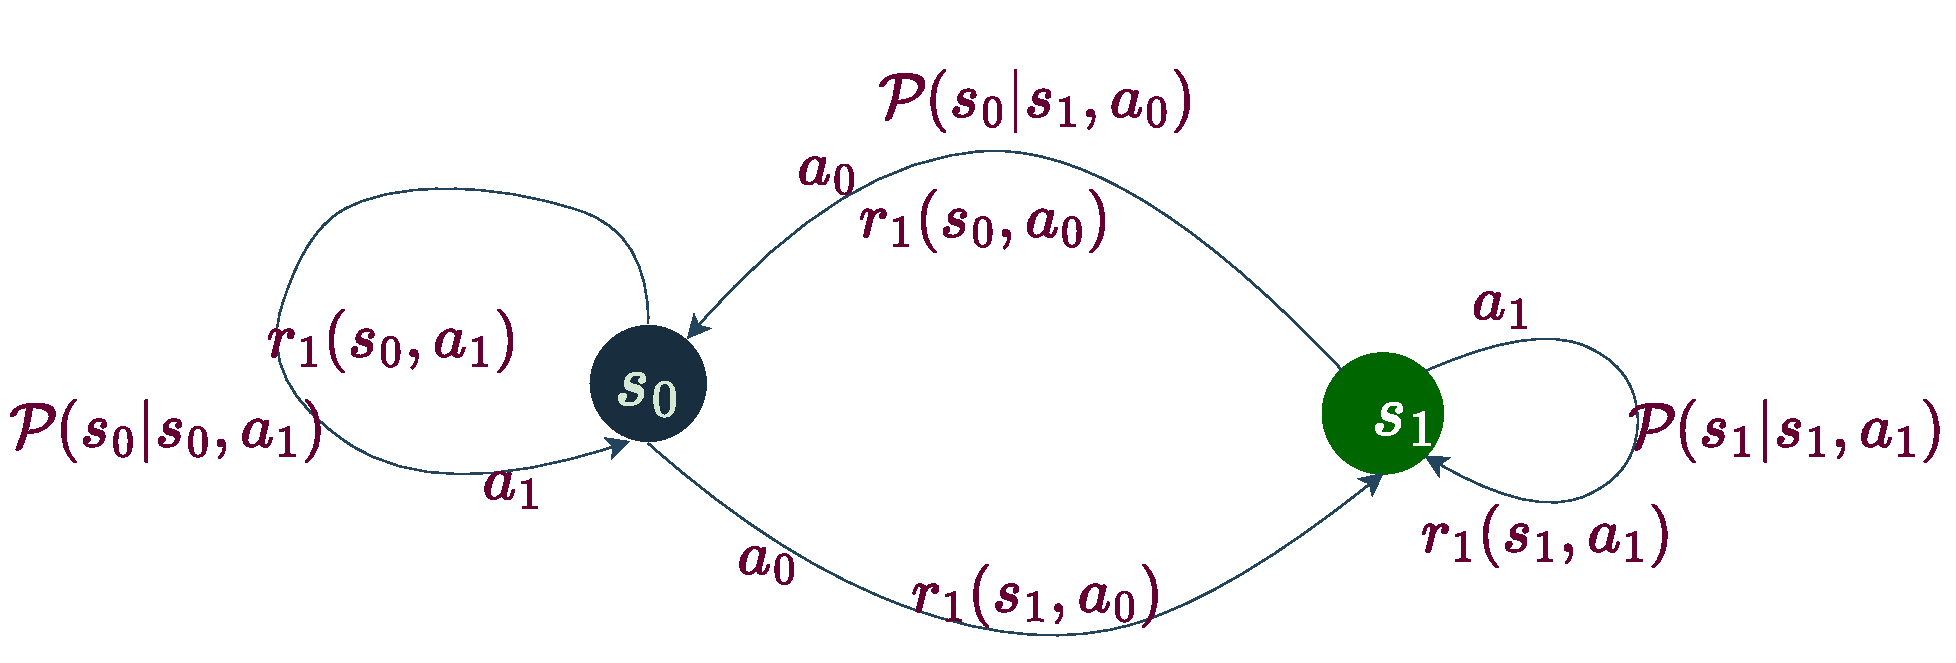
\includegraphics[width=0.95\textwidth]{figures/MarkovDecisionProcess.pdf}
    \end{center}

\end{frame}
%------------------------------------------------


\begin{frame}{A simple MDP}
        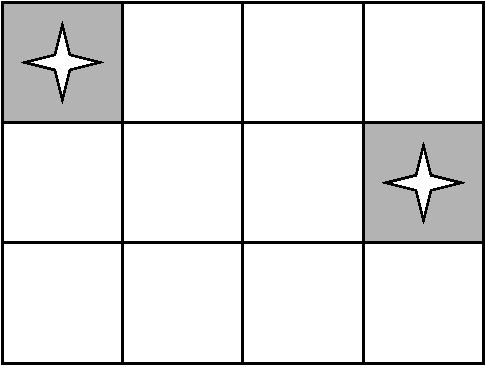
\includegraphics[width=0.25\textwidth]{figures/SimpleMDP.pdf}

actions $a=\{ 	\uparrow, 	\downarrow 	\leftarrow, \rightarrow\}$

\vspace{10pt}
Set a negative reward for each transition, say $-1$.

\vspace{10pt}
\textbf{Objective: }reach one of the terminal states (greyed out) in the least number of actions
\end{frame}

%------------------------------------------------


\begin{frame}{A simple MDP}
\begin{columns}[c]
    \column{.40\textwidth} 


        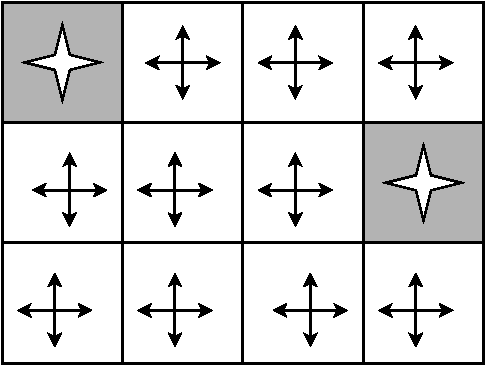
\includegraphics[width=0.99\textwidth]{figures/SimpleMDP_Random.pdf}

Random Policy

    \column{.40\textwidth} 

        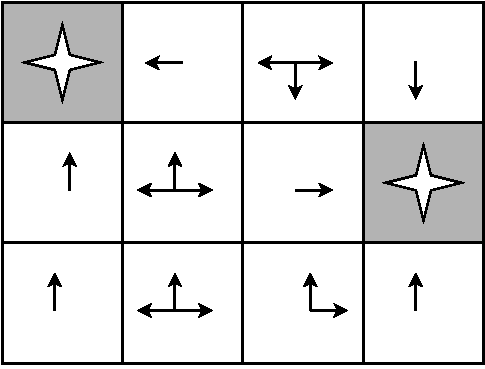
\includegraphics[width=0.99\textwidth]{figures/SimpleMDP_Optimal.pdf}

Optimal Policy

    
\end{columns}

\end{frame}
%------------------------------------------------

\begin{frame}{Objective in RL}
\begin{center}
    We want to find an optimal policy $\pi^*$ that maximizes the discounted sum of rewards.

    But as there is randomness (due to randomness in the initial state, transition probability, etc.), we say \textbf{we want to find an optimal policy $\pi^*$ that maximizes the expected discounted sum of rewards.}
\end{center}

Formally,

$$
\pi^* = \argmax_\pi  \Ebb\bigg[ \sum_{t\geq 0} \gamma^t r_t | \pi \bigg]
$$
    
\end{frame}
%------------------------------------------------

%------------------------------------------------

\begin{frame}{How good is a state?}
    Following a policy, we get a sequence of states and actions (and rewards associated with them): $s_0, a_0, r_0, s_1, a_1, r_1, \cdots $. So how to quantify the goodness of the state the agent arrives?
\end{frame}


%---------------------------------------------

\begin{frame}{Value Function}
The value function specifies how good it is for an agent to be in a particular state with a policy $\pi$. It is an expected cumulative reward following a policy from the state $s$:

$$
V^\pi (s) = \Ebb \bigg[ \sum_{t\geq 0} \gamma^t r_t | s_0 = s, \pi \bigg]
$$
    
\end{frame}


\begin{frame}{Simple Example: 2-State MDP}
    
    \vspace{0.5cm}
    \begin{center}
    \large{
    \begin{tabular}{ll}
    States: & S1, S2 \\
    Actions: & A, B \\
    Discount factor: & $\gamma = 0.9$ \\
    Time horizon: & 3 steps
    \end{tabular}
    }
    \end{center}
\end{frame}

\begin{frame}{Transition Probabilities \& Rewards: State S1}
    
    \vspace{0.5cm}
    \begin{center}
    \large{
    \textbf{When in state S1:}
    }
    \end{center}
    
    \vspace{0.5cm}
    \begin{center}
    \large{
    Action A: \\
    80\% chance to stay in S1 with reward +1 \\
    20\% chance to go to S2 with reward +0
    }
    \end{center}
    
    \vspace{0.5cm}
    \begin{center}
    \large{
    Action B: \\
    30\% chance to stay in S1 with reward +2 \\
    70\% chance to go to S2 with reward -1
    }
    \end{center}
\end{frame}

\begin{frame}{Transition Probabilities \& Rewards: State S2}
    
    \vspace{0.5cm}
    \begin{center}
    \large{
    \textbf{When in state S2:}
    }
    \end{center}
    
    \vspace{0.5cm}
    \begin{center}
    \large{
    Action A: \\
    40\% chance to go to S1 with reward +0 \\
    60\% chance to stay in S2 with reward +1
    }
    \end{center}
    
    \vspace{0.5cm}
    \begin{center}
    \large{
    Action B: \\
    10\% chance to go to S1 with reward +5 \\
    90\% chance to stay in S2 with reward +2
    }
    \end{center}
    \end{frame}
    

    \begin{frame}{Policy Evaluation}
        
        \vspace{0.5cm}
        \large{Let's evaluate two different policies:}
        
        \vspace{0.5cm}
        \begin{center}
        \large{
        Policy $\pi_1$: Always choose Action A regardless of state
        }
        \end{center}
        
        \vspace{0.5cm}
        \begin{center}
        \large{
        Policy $\pi_2$: Always choose Action B regardless of state
        }
        \end{center}
    \end{frame}

    \begin{frame}
        \frametitle{Recursive Value Calculation: Policy $\pi_1$}
        
        \vspace{0.5cm}
        \begin{center}
        \large{For Policy $\pi_1$ (always A):}
        \end{center}
        
        \vspace{0.5cm}
        \begin{multiequation}
        \large{V^{\pi_1}(S1)} &= \large{1 + 0.9[0.8 \cdot V^{\pi_1}(S1) + 0.2 \cdot V^{\pi_1}(S2)]}\\
        \vspace{0.3cm}
        \large{V^{\pi_1}(S2)} &= \large{1 + 0.9[0.4 \cdot V^{\pi_1}(S1) + 0.6 \cdot V^{\pi_1}(S2)]}
        \end{multiequation}

        $\gamma = 0.9$. Assume initial value of $V^{\pi_1}(S1) = 0$ and  $V^{\pi_1}(S2) = 0$.
        
        \vspace{0.5cm}
        \begin{center}
        \large{Starting from S1, over 3 steps: $V^{\pi_1}(S1) \approx 2.71$}
        \end{center}
    \end{frame}

    \begin{frame}{Recursive Value Calculation: Policy $\pi_2$}
    
    \vspace{0.5cm}
    \begin{center}
    \large{For Policy $\pi_2$ (always B):}
    \end{center}
    
    \vspace{0.5cm}
    \begin{multiequation}
    \large{V^{\pi_2}(S1)} &= \large{2 + 0.9[0.3 \cdot V^{\pi_2}(S1) + 0.7 \cdot V^{\pi_2}(S2)]}\\
    \vspace{0.3cm}
    \large{V^{\pi_2}(S2)} &= \large{2 + 0.9[0.1 \cdot V^{\pi_2}(S1) + 0.9 \cdot V^{\pi_2}(S2)]}
    \end{multiequation}
    
    $\gamma = 0.9$. Assume initial value of $V^{\pi_1}(S1) = 0$ and  $V^{\pi_1}(S2) = 0$.

    \vspace{0.5cm}
    \begin{center}
    \large{Starting from S1, over 3 steps: $V^{\pi_2}(S1) \approx $}
    \end{center}
    \end{frame}
    
    \begin{frame}{Finding the Optimal Policy}
    
    \vspace{1cm}
    \begin{center}
    \large{Policy $\pi_1$ (always A) yields $V^{\pi_1}(S1) \approx 2.71$}
    \end{center}
    
    \vspace{0.8cm}
    \begin{center}
    \large{Policy $\pi_2$ (always B) yields $V^{\pi_2}(S1) \approx ~~~~~~ $}
    \end{center}
    
    \vspace{1cm}
    \begin{center}
    \large{\textbf{Therefore, $\pi^* = ~~~~~~~~~~~~ $ is our optimal policy}}
    \end{center}
    \end{frame}
    
\begin{frame}{How good is a state action-pair?}
In addition, we also need to quantify the goodness of a state-action pair.
    
\end{frame}

%---------------------------------------------

\begin{frame}{Q Function}
The Q function maps each state-action pair to a real number, representing the expected reward over the long run starting from that state and taking that action.

$$
Q  ^\pi (s, a) = \Ebb\bigg[ \gamma^t r_t | s_0 = s, a_0 = a, \pi  \bigg]
$$
    
\end{frame}

%---------------------------------------------


\begin{frame}{Bellman Equation}
    \small
$Q^*$ is the optimal Q-value which is the maximum expected cumulative reward achievable from the given state-action pair under the given policy:

$$
Q^*(s, a) = \max_\pi  \Ebb\bigg[ \gamma^t r_t | s_0 = s, a_0 = a, \pi  \bigg]
$$

$Q^*$ satisfies a recursive relation called \textbf{Bellman Equation:}

$$
Q^*(s, a) = \Ebb_{s_{t+1}\sim P(\cdot | s,a) } \bigg[ r 
    + \gamma \max_{a'} Q^*(s_{t+1}, a_{t+1}) | s, a\bigg]
$$

{\textcolor{red}{which essentially tells that if I know the optimal state-action pair for the next time-step, quantified using $Q^*(s_{t+1}, a_{t+1})$, then the optimal strategy is to take the action that maximizes the reward $r + \gamma Q^*(s_{t+1}, a_{t+1}) $. 
}}

$s_{t+1}\sim P(\cdot | s, a) $ tells you that the next state is chosen stochastically as per the transition probability.
\end{frame}


%---------------------------------------------

\begin{frame}{Optimal Policy and Bellman Equation}
    \begin{center}
    \LARGE
        Hence, the optimal policy $\pi^*$ corresponds to taking the best action in any state as specified by $Q^*$.
    \end{center}
\end{frame}


%---------------------------------------------

\begin{frame}{Solving for Optimal Policy}

We use \textbf{value iteration algorithm} to solve for an optimal policy iteratively as follows:

$$
Q_{i+1} = \Ebb \bigg[ r + \gamma \max_{a'} Q_i(s_{t+1}, a_{t+1}) | s, a\bigg]
$$

until $Q_{i+1} \approx Q_{i}$, i.e. when convergence happens. In this case, we initialize $Q_0(s, a)$ to some arbitrary values for the given state-action pair.

\end{frame}


%---------------------------------------------

\begin{frame}{Solving for Optimal Policy: Use Dynamic Programming}

The recursion is solved using dynamic programming where a task is divided into multiple smaller tasks and their solutions are recursively combined to get the final solution.

\vspace{15pt}
A similar recursive equation can be constructed if we just work with the value function rather than the Q-function. 
    
\end{frame}


\begin{frame}{An Example Environment}
\small
    \begin{columns}
        \begin{column}{0.6\textwidth}
            \begin{tcolorbox}[colback=lightblue!30,colframe=blue!60!black,title=Grid World Setup]
                \begin{itemize}
                    \item 4 states (S0, S1, S2, S3)
                    \item S3 is terminal state with reward +10
                    \item All other transitions: reward 0
                    \item Discount factor $\gamma = 0.9$
                \end{itemize}
            \end{tcolorbox}


        \end{column}
        \begin{column}{0.4\textwidth}
            \begin{tcolorbox}[colback=lightorange!30,colframe=orange!60!black,title=Available Actions]
                Up, Down, Left, Right
            \end{tcolorbox}

            \begin{center}
                \begin{tikzpicture}[scale=0.9]
                    \draw[step=2cm,thick] (0,0) grid (4,4);
                    \node at (1,3) {S0};
                    \node at (3,3) {S1};
                    \node at (1,1) {S2};
                    \node[draw, fill=lightgreen!40, rounded corners] at (3,1) {S3 (+10)};
                    \draw[->, thick, red] (1,1) -- (2.8,1);
                    \draw[->, thick, red] (3,3) -- (3,1.2);
                    \draw[->, thick, red] (1,3) -- (1,1.2);
                \end{tikzpicture}
            \end{center}

        \end{column}
    \end{columns}
    
    
\end{frame}

\begin{frame}{Transition Model}
    \begin{tcolorbox}[colback=lightblue!10,colframe=blue!60!black,title=Stochastic Environment]
        \begin{itemize}
            \item Actions succeed with probability 0.8
            \item Actions fail (move in random other direction) with probability 0.2
            \item Moving into a wall keeps agent in same state
        \end{itemize}
    \end{tcolorbox}
    
    \begin{tblock}{Reminder}
        The Q-function represents expected long-term reward when taking action $a$ in state $s$.
    \end{tblock}
\end{frame}

\begin{frame}{Value Iteration Process}
    \footnotesize
    \begin{tcolorbox}[enhanced,colback=white,colframe=blue!75!black]
        \begin{multiequation}
            Q_{i+1}(s,a) = \mathbb{E}\left[r + \gamma \max_{a'} Q_i(s_{t+1}, a') \mid s, a\right]
        \end{multiequation}
    \end{tcolorbox}
    
    \begin{center}
        Starting condition: $Q_0(s,a) = 0$ for all state-action pairs
    \end{center}
    
    \vspace{0.1cm}
    \begin{columns}
        \begin{column}{0.5\textwidth}
            \begin{tcolorbox}[colback=lightblue!20,colframe=blue!60!black,title=Iteration 1]
                \begin{multiequation}
                    Q_1(\text{S2}, \text{Right}) &= 0.8 \times (10 + 0.9 \times 0)\\
                    &+ 0.2 \times (0 + 0.9 \times 0)\\
                    &= \alert{8.0}
                \end{multiequation}
            \end{tcolorbox}
        \end{column}
        \begin{column}{0.5\textwidth}
            \begin{tcolorbox}[colback=lightblue!20,colframe=blue!60!black,title=Iteration 1]
                \begin{multiequation}
                    Q_1(\text{S0}, \text{Down}) &= 0.8 \times (0 + 0.9 \times 0)\\
                    &+ 0.2 \times (0 + 0.9 \times 0)\\
                    &= \alert{0.0}
                \end{multiequation}
            \end{tcolorbox}
        \end{column}
    \end{columns}
\end{frame}


\begin{frame}{Continue Value Iteration}
    \small
    \begin{columns}
        \begin{column}{0.5\textwidth}
            \begin{tcolorbox}[colback=lightorange!20,colframe=orange!60!black,title=Iteration 2]
                \begin{multiequation}
                    Q_2(\text{S2}, \text{Right}) &\approx 8.96\\
                    Q_2(\text{S1}, \text{Down}) &\approx 8.96\\
                    Q_2(\text{S0}, \text{Right}) &\approx 6.24
                \end{multiequation}
            \end{tcolorbox}
        \end{column}
        \begin{column}{0.5\textwidth}
            \begin{tcolorbox}[colback=lightgreen!20,colframe=green!60!black,title=Iteration 3]
                \begin{multiequation}
                    Q_3(\text{S0}, \text{Down}) & = 7.74
                \end{multiequation}
                Values start propagating backward!
            \end{tcolorbox}
        \end{column}
    \end{columns}
    
    \vspace{0.5cm}
    \begin{tblock}{}
        The Bellman equation propagates reward information backward from rewarding states.
    \end{tblock}
\end{frame}


\begin{frame}{}
    \footnotesize

    \begin{tcolorbox}[colback=lightblue!10,colframe=darkRose!60!black,title=Q* Values After Convergence (Converged after 9 iterations!)]
        \begin{center}
            \begin{tabular}{lcc}
                \toprule
                \textbf{State} & \textbf{Action} & \textbf{Q* Value} \\
                \midrule
                \rowcolor{lightblue!20} S0 & Right & 8.57 \\
                S0 & Down & \cellcolor{lightgreen!30}\textbf{8.57} \\
                \rowcolor{lightblue!20} S1 & Left & 8.00 \\
                S1 & Down & \cellcolor{lightgreen!30}\textbf{9.68} \\
                \rowcolor{lightblue!20} S2 & Up & 8.00 \\
                S2 & Right & \cellcolor{lightgreen!30}\textbf{9.68} \\
                \bottomrule
            \end{tabular}
        \end{center}
    \end{tcolorbox}
    
    \begin{center}
        \begin{tikzpicture}[scale=0.8]
            \draw[step=2cm,thick] (0,0) grid (4,4);
            \node at (1,3) {S0};
            \node at (3,3) {S1};
            \node at (1,1) {S2};
            \node[draw, fill=lightgreen!40, rounded corners] at (3,1) {S3 (+10)};
            \draw[->, ultra thick, red] (1,3) -- (1,1.2);
            \draw[->, ultra thick, red] (3,3) -- (3,1.2);
            \draw[->, ultra thick, red] (1,1) -- (2.8,1);
        \end{tikzpicture}
    \end{center}
\end{frame}

\begin{frame}{}
    \footnotesize
    \begin{tcolorbox}[colback=lightgreen!30,colframe=indianRed!60!black,title=Optimal Policy $\pi^*$]
        For each state, choose action with highest Q* value:
        \begin{center}
            \begin{tabular}{lcc}
                \toprule
                \textbf{State} & \textbf{Best Action} & \textbf{Q* Value} \\
                \midrule
                \rowcolor{lightorange!20} S0 & Down & 8.57 \\
                \rowcolor{lightorange!20} S1 & Down & 9.68 \\
                \rowcolor{lightorange!20} S2 & Right & 9.68 \\
                \bottomrule
            \end{tabular}
        \end{center}
    \end{tcolorbox}
    
    \begin{tblock}{}
        Q-values quantify the ``goodness" of each state-action pair in terms of expected long-term reward.
    \end{tblock}
    
    \vspace{0.3cm}
    \begin{center}
        The optimal policy efficiently guides the agent toward the high-reward terminal state.
    \end{center}
\end{frame}



\begin{frame}{State-Action Rewards $R(s,a)$}

    \begin{columns}
        \column{0.7\textwidth}
        \begin{itemize}
            \item Rewards depend only on the current state and action taken
            \item Notation: $R(s,a)$ or $R_{sa}$
            \item Mathematical definition:
            \begin{multiequation}
                R(s,a) &= \mathbb{E}[r_t | s_t = s, a_t = a] \\
                &= \sum_{s' \in S} P(s'|s,a) \cdot r(s,a)
            \end{multiequation}
            \item Example: In a grid world, stepping on a trap (action) while in a specific location (state) incurs a penalty, regardless of where you end up
        \end{itemize}
        \column{0.3\textwidth}
        \begin{tikzpicture}[node distance=2cm, auto, thick]
            \node[state, draw=blue] (s0) {$s_0$};
            \node[state, draw=blue, right of=s0] (s1) {$s_1$};
            
            \draw[->] (s0) edge[bend left, above] node{$a_0: +1$} (s1);
            \draw[->] (s0) edge[loop above] node{$a_1: 0$} (s0);
            \draw[->] (s1) edge[bend left, below] node{$a_0: 0$} (s0);
            \draw[->] (s1) edge[loop above] node{$a_1: +2$} (s1);
        \end{tikzpicture}
    \end{columns}
    \end{frame}
    
    \begin{frame}{State-Only Rewards $R(s)$}
        \begin{columns}
            \column{0.75\linewidth}
            \begin{itemize}
                \item Rewards depend only on the state the agent is in
                \item Notation: $R(s)$ or $R_s$
                \item Mathematical definition:
                \begin{multiequation}
                    R(s) &= \mathbb{E}[r_t | s_t = s] 
                \end{multiequation}
                \item Value functions with state-only rewards:
                \begin{multiequation}
                    V^\pi(s) &= R(s) + \gamma \sum_{s' \in S} P(s'|s,\pi(s)) V^\pi(s') \\
                    Q^\pi(s,a) &= R(s) + \gamma \sum_{s' \in S} P(s'|s,a) V^\pi(s')
                \end{multiequation}
                \item Example: Treasure on specific grid locations gives reward just for being there
            \end{itemize}
            
            \column{0.25\linewidth}
            \begin{tikzpicture}[node distance=2cm, auto, thick]
                \node[state, draw=blue] (s0) {$s_0: +1$};
                \node[state, draw=blue, right of=s0] (s1) {$s_1: +3$};
                
                \draw[->] (s0) edge[bend left, above] node{$a_0$} (s1);
                \draw[->] (s0) edge[loop above] node{$a_1$} (s0);
                \draw[->] (s1) edge[bend left, below] node{$a_0$} (s0);
                \draw[->] (s1) edge[loop above] node{$a_1$} (s1);
            \end{tikzpicture}
        \end{columns}
    \end{frame}
    
    \begin{frame}{State-Action-State Rewards $R(s,a,s')$}
        \begin{columns}
            \column{0.9\linewidth}
            \begin{itemize}
                \item Rewards depend on the current state, action taken, and the resulting next state
                \item Notation: $R(s,a,s')$ or $R_{sas'}$
                \item Mathematical definition:
                \begin{multiequation}
                    R(s,a,s') &= \mathbb{E}[r_t | s_t = s, a_t = a, s_{t+1} = s']
                \end{multiequation}
                \item Bellman equation with state-action-state rewards:
                \begin{multiequation}
                    V^\pi(s) &= \sum_{a \in A} \pi(a|s) \sum_{s' \in S} P(s'|s,a) [R(s,a,s') + \gamma V^\pi(s')]
                \end{multiequation}
                \item Example: Reward for successfully jumping over a pit (transition from initial state to goal state via jump action)
            \end{itemize}
            
    \end{columns}

    

    \end{frame}
    
    \begin{frame}{State-Action-State Rewards: Matrix Form}
        \footnotesize
    For an MDP with 2 states and 2 actions, $R(s,a,s')$ can be represented as matrices:
    
    For action $a_0$:
    \[
    R_{a_0} = 
    \begin{bmatrix}
    R(s_0, a_0, s_0) & R(s_0, a_0, s_1) \\
    R(s_1, a_0, s_0) & R(s_1, a_0, s_1) 
    \end{bmatrix}
    =
    \begin{bmatrix}
    1 & 2 \\
    -1 & 0 
    \end{bmatrix}
    \]
    
    For action $a_1$:
    \[
    R_{a_1} = 
    \begin{bmatrix}
    R(s_0, a_1, s_0) & R(s_0, a_1, s_1) \\
    R(s_1, a_1, s_0) & R(s_1, a_1, s_1) 
    \end{bmatrix}
    =
    \begin{bmatrix}
    0 & 1 \\
    3 & 2 
    \end{bmatrix}
    \]
    
    The expected reward for taking action $a$ in state $s$ is:
    \[
    R(s,a) = \sum_{s' \in S} P(s'|s,a) \cdot R(s,a,s')
    \]
    \end{frame}
    
    \begin{frame}{Expected Rewards: Converting Between Forms}
        \footnotesize
    \begin{itemize}
        \item Converting from $R(s,a,s')$ to $R(s,a)$:
        \begin{multiequation}
            R(s,a) &= \sum_{s' \in S} P(s'|s,a) \cdot R(s,a,s')
        \end{multiequation}
        
        \item Converting from $R(s,a)$ to expected rewards:
        \begin{multiequation}
            R(s) &= \sum_{a \in A} \pi(a|s) \cdot R(s,a)
        \end{multiequation}
        
        \item Bellman equation using $R(s,a)$:
        \begin{multiequation}
            V^\pi(s) &= \sum_{a \in A} \pi(a|s) \left[ R(s,a) + \gamma \sum_{s' \in S} P(s'|s,a) V^\pi(s') \right]
        \end{multiequation}
    \end{itemize}
    \end{frame}
    
    \begin{frame}{Practical Example: Grid World Rewards}
        \footnotesize
    \begin{columns}
    \column{0.5\textwidth}
    \textbf{State-Action Rewards $R(s,a)$}
    \begin{multiequation}
    R(s, \text{up}) &= 
    \begin{cases}
    -1, & \text{if } s \text{ is regular cell} \\
    -10, & \text{if } s \text{ is adjacent to pit}
    \end{cases} \\
    R(s, \text{right}) &= 
    \begin{cases}
    -1, & \text{if } s \text{ is regular cell} \\
    +10, & \text{if } s \text{ is adjacent to goal}
    \end{cases}
    \end{multiequation}
    
    \column{0.5\textwidth}
    \textbf{State-Only Rewards $R(s)$}
    \begin{multiequation}
    R(s) &= 
    \begin{cases}
    -1, & \text{if } s \text{ is regular cell} \\
    -100, & \text{if } s \text{ is pit} \\
    +100, & \text{if } s \text{ is goal}
    \end{cases}
    \end{multiequation}
    
    \end{columns}
    
    \vspace{0.5cm}
    \textbf{State-Action-State Rewards $R(s,a,s')$}
    \begin{multiequation}
    R(s,a,s') &= 
    \begin{cases}
    -1, & \text{if } s' \text{ is regular cell} \\
    -100, & \text{if } s' \text{ is pit} \\
    +100, & \text{if } s' \text{ is goal} \\
    -10, & \text{if action fails (hits wall)}
    \end{cases}
    \end{multiequation}
    \end{frame}
    
    \begin{frame}{Comparison of Reward Structures}
        \footnotesize
    \begin{tabular}{|p{3cm}|p{3.5cm}|p{3.5cm}|}
    \hline
    \textbf{Reward Type} & \textbf{Advantages} & \textbf{Disadvantages} \\
    \hline
    State-Only $R(s)$ & Simple to understand and implement & Cannot reward specific behaviors or transitions \\
    \hline
    State-Action $R(s,a)$ & Can encourage/discourage specific actions in specific states & Cannot distinguish between different outcomes of the same action \\
    \hline
    State-Action-State $R(s,a,s')$ & Most expressive; can reward specific transitions & More complex to design and implement \\
    \hline
    \end{tabular}
    
    \vspace{0.5cm}
    \begin{itemize}
        \item Choice of reward structure depends on:
        \begin{itemize}
            \item Task requirements
            \item Available information
            \item Desired agent behavior
        \end{itemize}
        \item Any reward structure can be converted to another with proper mathematical transformations
    \end{itemize}
    \end{frame}
    
    \begin{frame}{Relationship to Optimal Policies}
        \footnotesize
    The optimal policy $\pi^*$ maximizes the expected discounted sum of rewards:
    
    \begin{multiequation}
    \pi^* &= \arg\max_\pi \mathbb{E}_\pi\left[\sum_{t=0}^{\infty} \gamma^t r_t \right] \\
    &= \arg\max_\pi \mathbb{E}_\pi\left[\sum_{t=0}^{\infty} \gamma^t R(s_t, a_t) \right]
    \end{multiequation}
    
    Optimal value functions:
    \begin{multiequation}
    V^*(s) &= \max_a \left[ R(s,a) + \gamma \sum_{s' \in S} P(s'|s,a) V^*(s') \right] \\
    Q^*(s,a) &= R(s,a) + \gamma \sum_{s' \in S} P(s'|s,a) \max_{a'} Q^*(s',a')
    \end{multiequation}
    
    The choice of reward structure can significantly impact the learned policy!
    \end{frame}
    
    \begin{frame}{Reward Design Principles}
        \footnotesize
    \begin{itemize}
        \item \textbf{Parsimony}: Use the simplest reward structure that captures the task requirements
        \item \textbf{Alignment}: Ensure rewards truly represent the desired behaviors and outcomes
        \item \textbf{Consistency}: Similar states/actions should receive similar rewards
        \item \textbf{Sparsity vs. Density}: Trade-off between sparse rewards (clearer signal) and dense rewards (easier learning)
        \item \textbf{Scale}: The magnitude of rewards should be proportional to their importance
        \item \textbf{Horizons}: Consider discount factor $\gamma$ in relation to reward time scales
    \end{itemize}
    
    \vspace{0.5cm}
    Reward design is often considered an art as much as a science in reinforcement learning!
    \end{frame}

    
%---------------------------------------------


\begin{frame}{Let's do some coding}
    \begin{center}
        \LARGE
        \url{https://github.com/rahulbhadani/CPE487587_SP26/blob/master/Code/Chapter_09_Reinforcement_Learning.ipynb}
    \end{center}
\end{frame}


%---------------------------------------------

\section{Deep Reinforcement Learning}
%---------------------------------------------

\begin{frame}{}
    \begin{center}
    \huge \bf \color{DarkBlue}
    Deep Reinforcement Learning
    
\end{center}

\end{frame}

%---------------------------------------------


\begin{frame}{Why Deep Reinforcement Learning?}
    The use of the Bellman Equation and Dynamic Programming to find optimal policy requires computing $Q(s, a)$ for every state-action pair. This can be computationally intractable for most problems such as a autonomous driving where the state is continuous (denoted by speed, acceleration, etc.9+).
    \LARGE
    \begin{center}
        \vspace{10pt}
    In such a case, we use a deep neural network as a function approximation for $Q(s, a)$.
    \end{center}
    
\end{frame}



%---------------------------------------------

\begin{frame}{Deep Learning Algorithms}
\begin{columns}[c]
    \column{.50\textwidth} 

\begin{tblock}{Value Learning (Q-Learning)}
    \begin{itemize}
        \item Model $Q(s, a)$ using deep learning, 
        \item then $a = \argmax_a Q(s, a)$
    \end{itemize}
\end{tblock}

    \column{.50\textwidth} 
    
\begin{tblock}{Policy Learning}
    \begin{itemize}
        \item Model $\pi(s)$ using deep learning, 
        \item then $\text{Sample }a \sim \pi(s)$
    \end{itemize}
\end{tblock}
\end{columns}
    
\end{frame}

%---------------------------------------------

\begin{frame}{Q-Learning}
\begin{columns}[c]
    \column{.70\textwidth} 
    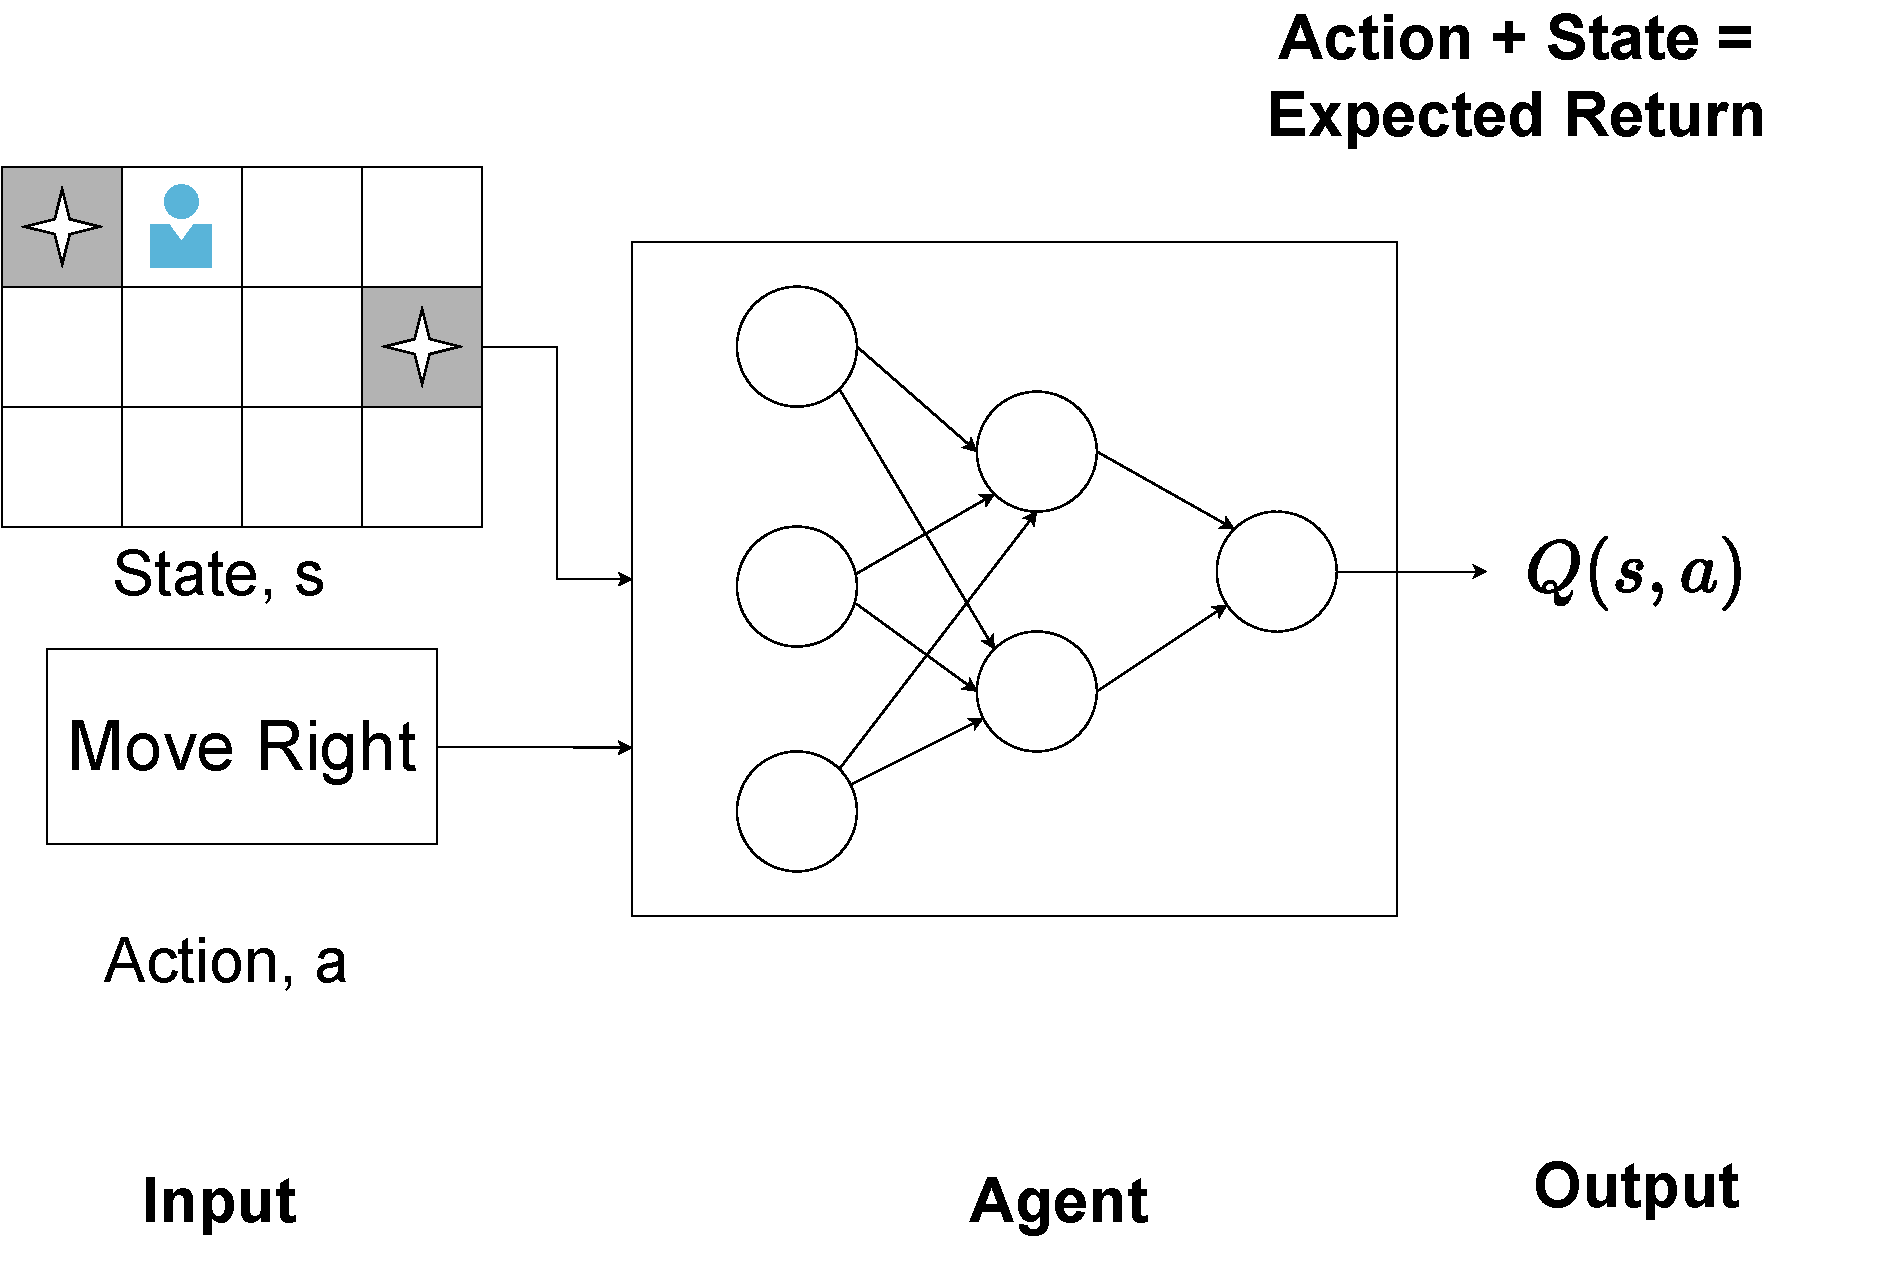
\includegraphics[width=0.80\textwidth]{figures/QLearning.pdf}
    \column{.30\textwidth} 
    Very inefficient for a large set of actions.
\end{columns}
\end{frame}

%---------------------------------------------

\begin{frame}{Q-Learning}
\begin{columns}[c]
    \column{.70\textwidth} 
    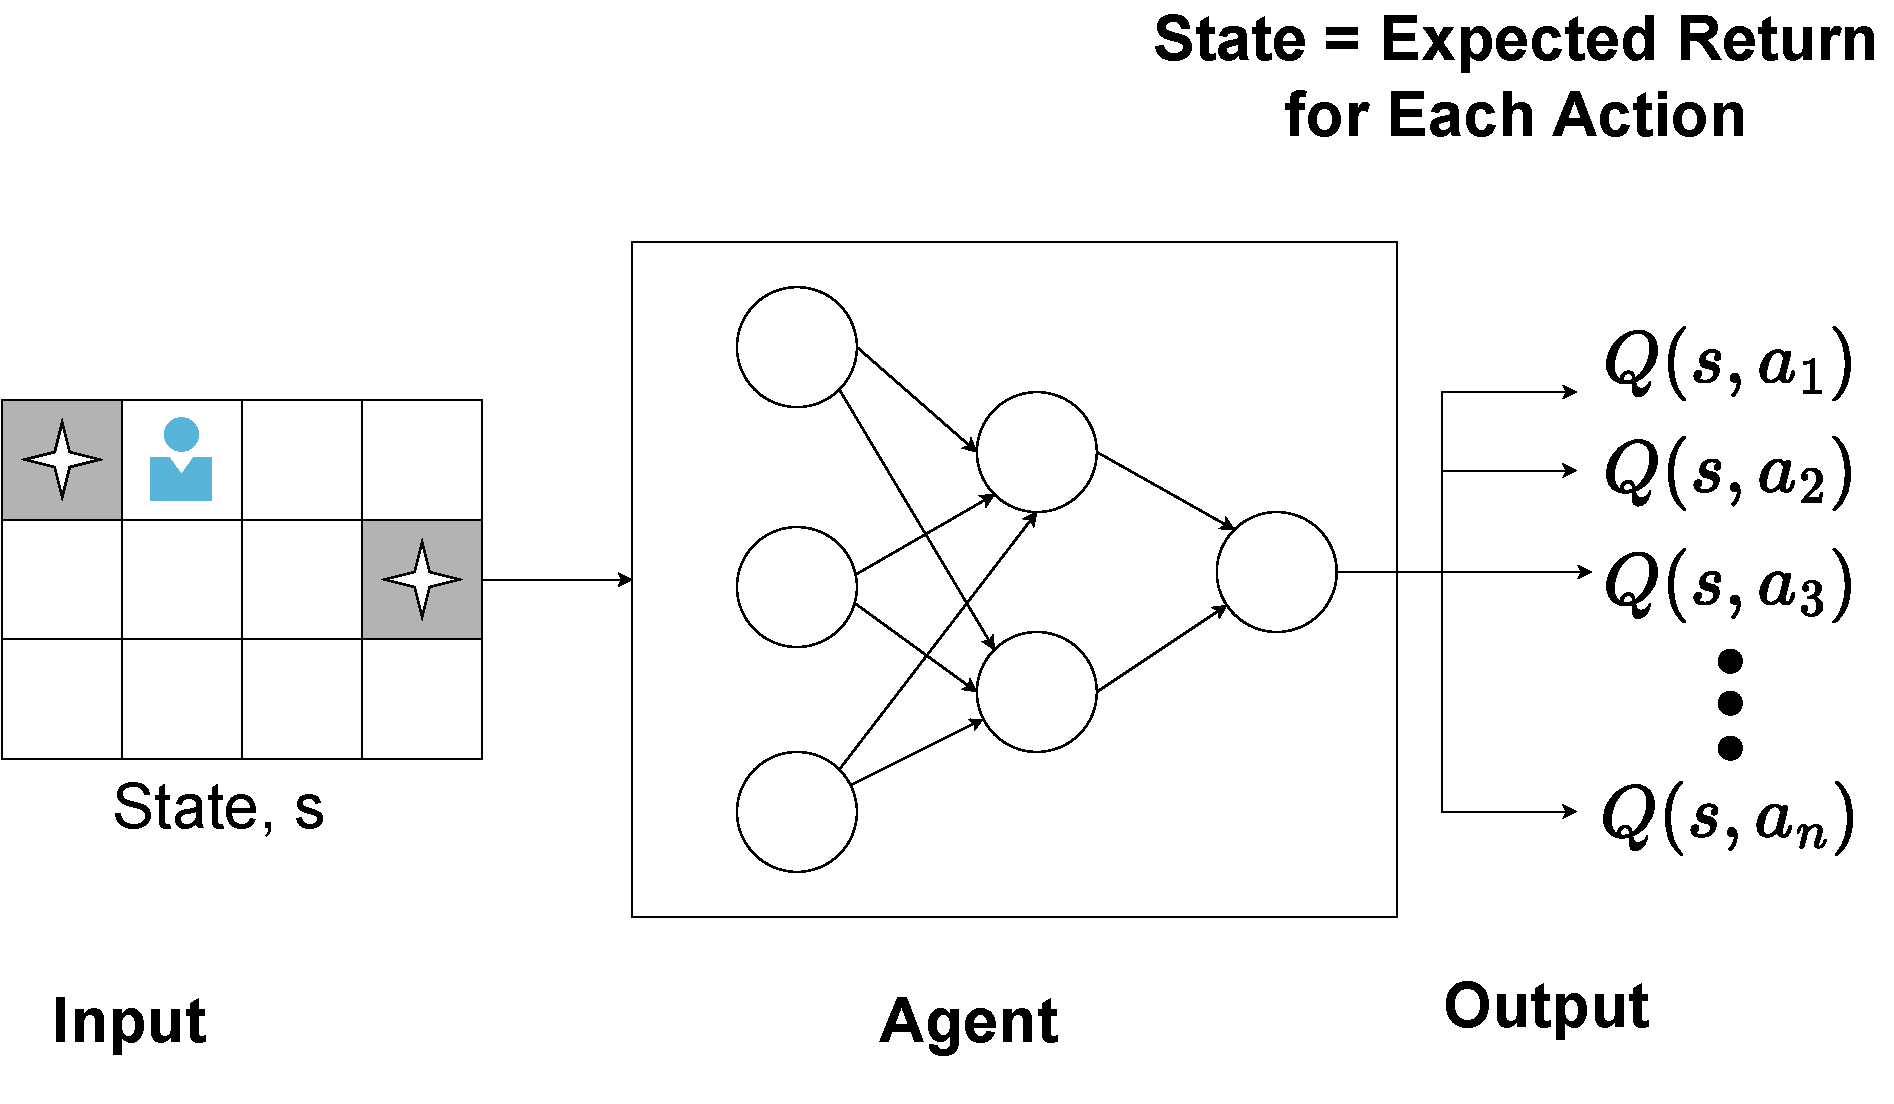
\includegraphics[width=0.80\textwidth]{figures/QLearning2.pdf}
\column{.30\textwidth} 
Take action based on the highest value of $Q$.

\end{columns}
\end{frame}

%---------------------------------------------

\begin{frame}{Q-Learning}
\begin{columns}[c]
    \column{.70\textwidth} 
    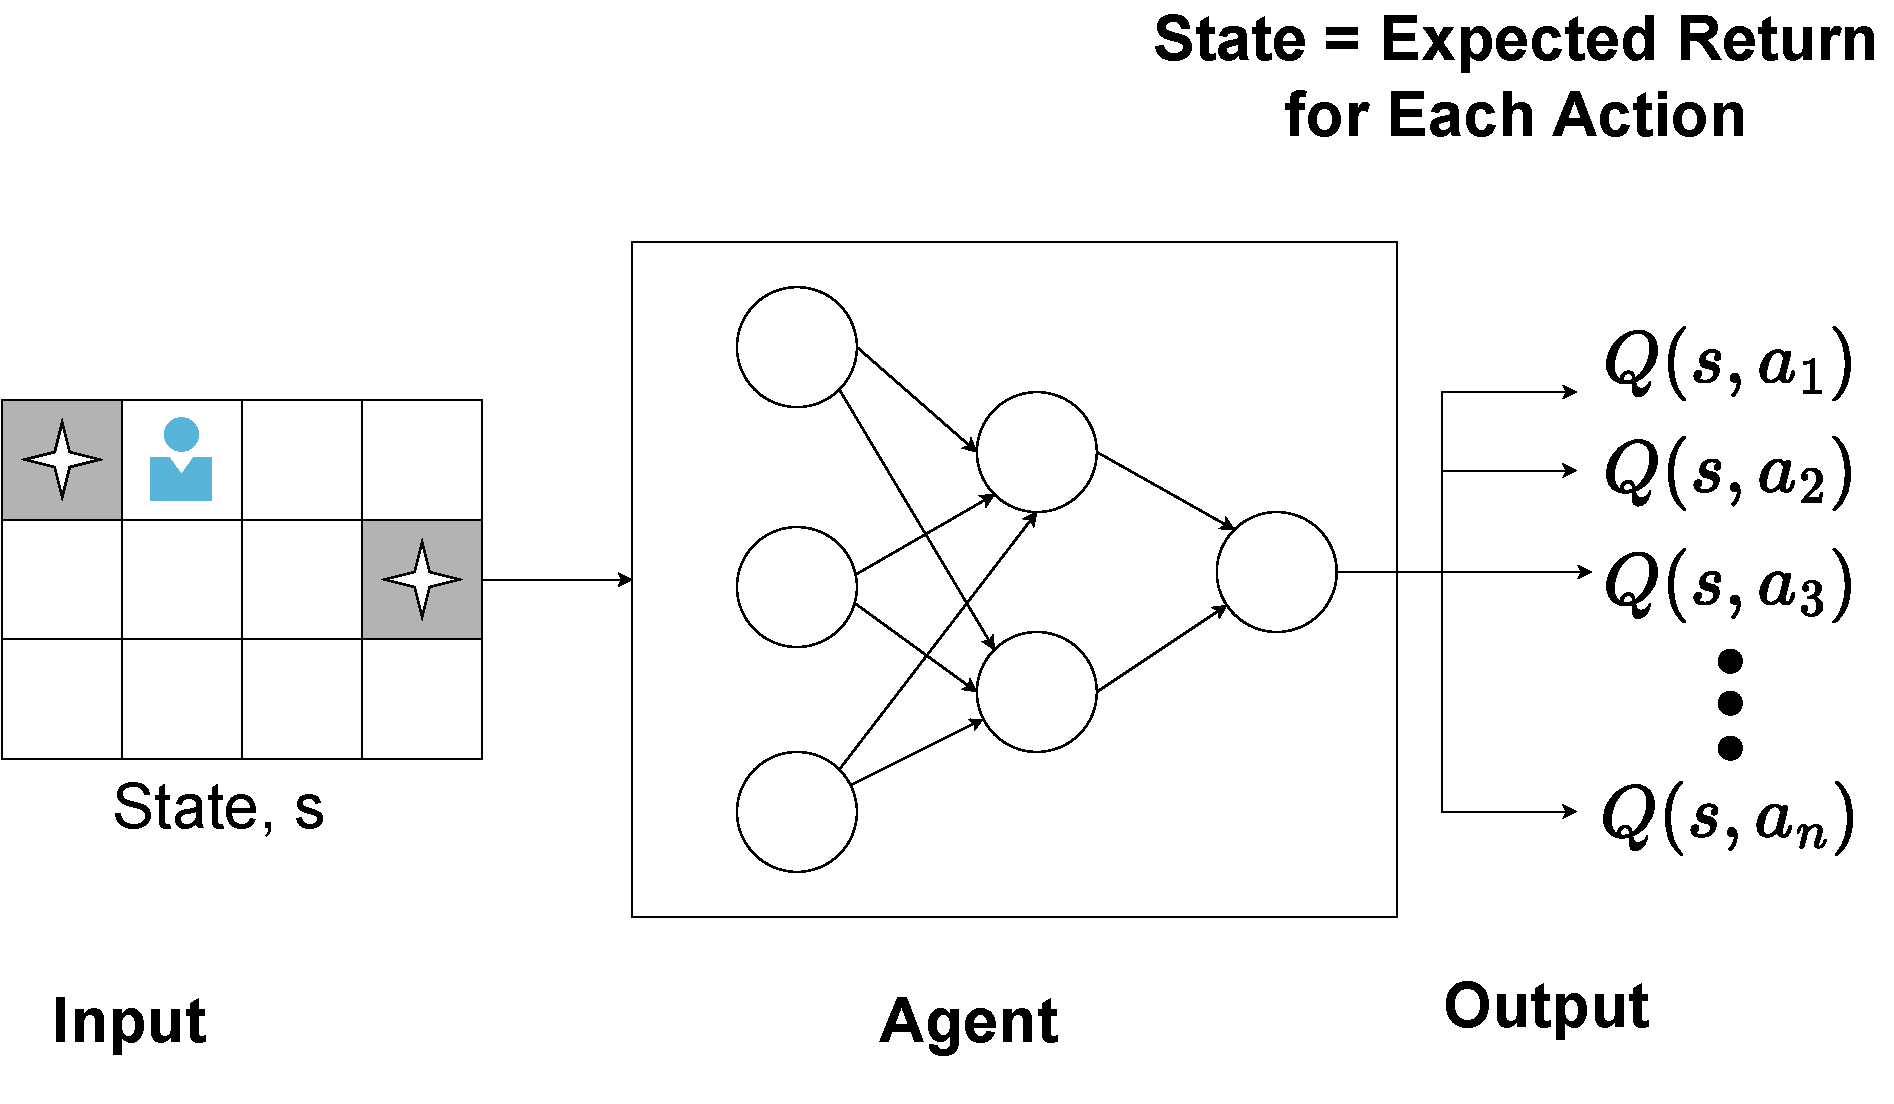
\includegraphics[width=0.80\textwidth]{figures/QLearning2.pdf}
\column{.30\textwidth} 

\vspace{10pt}

What happens when we take all the best actions?


\end{columns}
\end{frame}

%---------------------------------------------

\begin{frame}{Q-Learning}
\begin{columns}[c]
    \column{.70\textwidth} 
    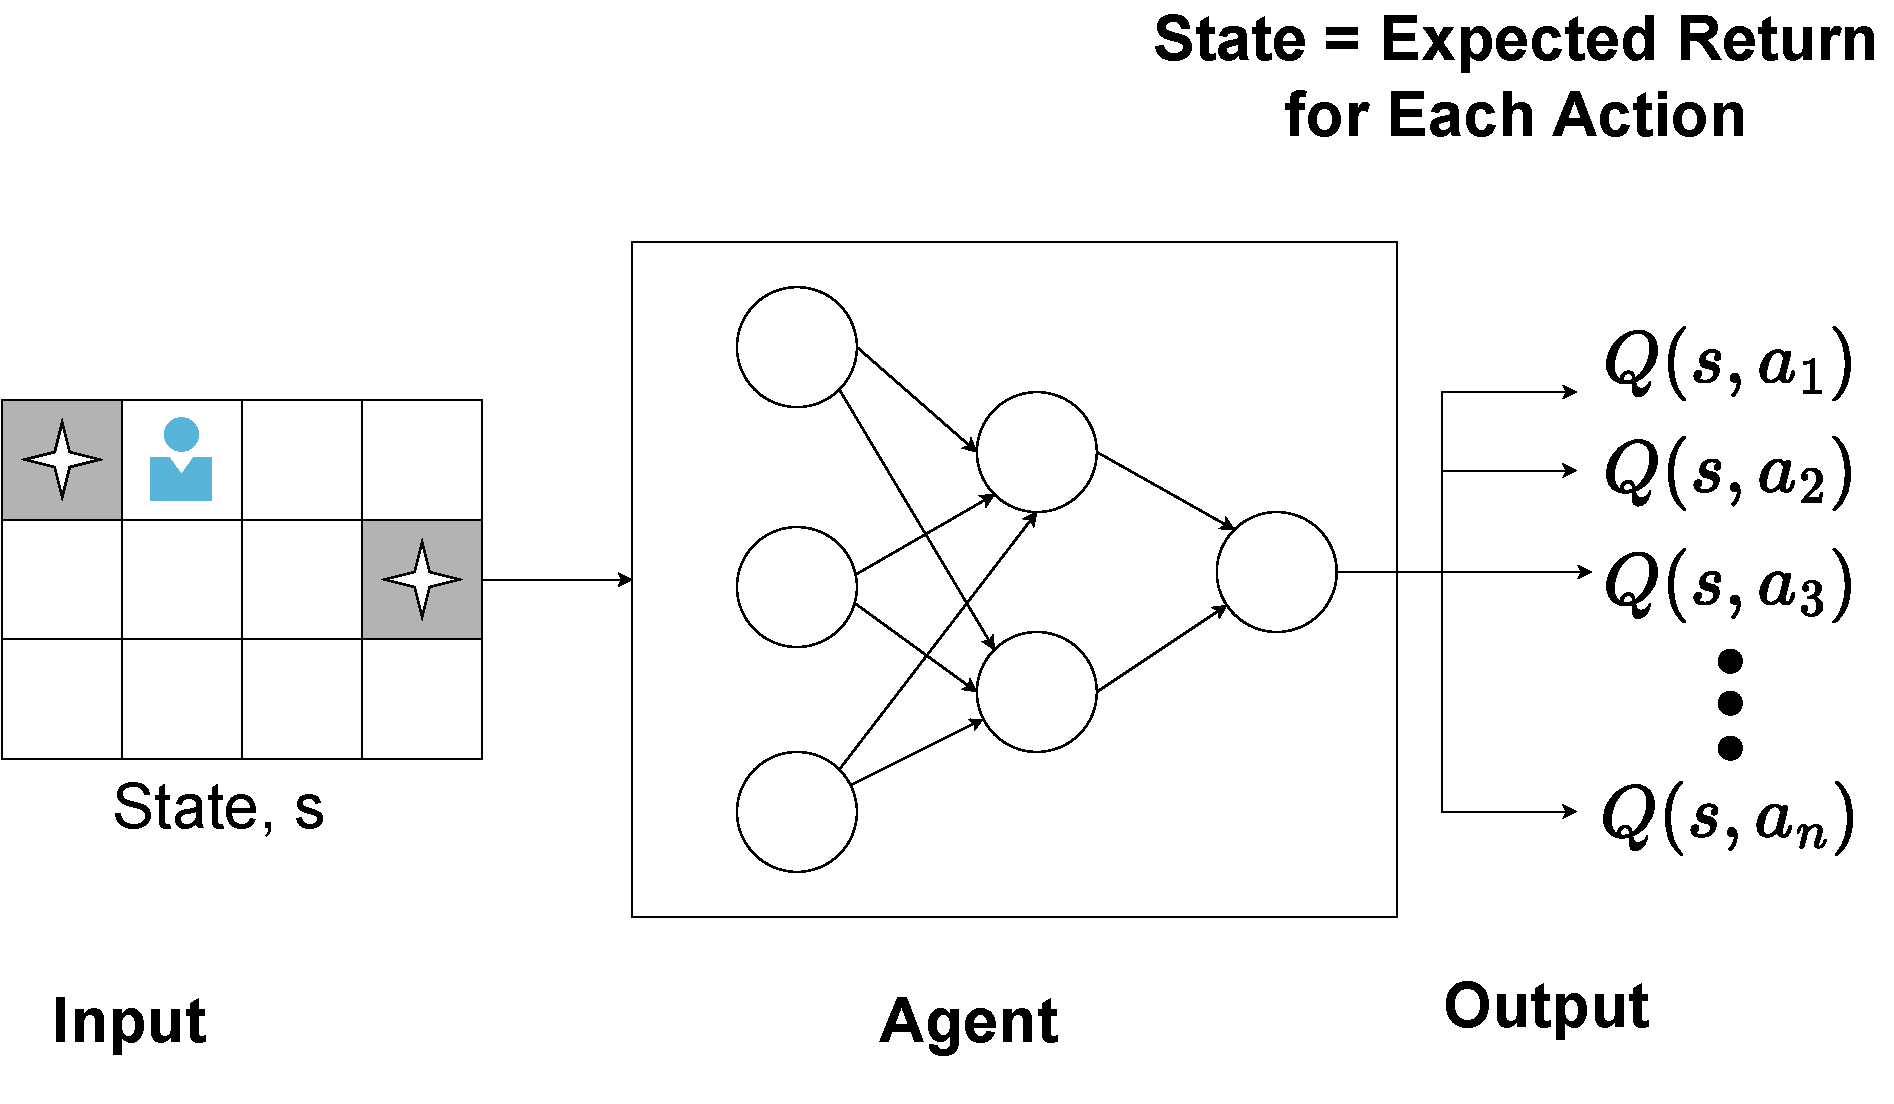
\includegraphics[width=0.80\textwidth]{figures/QLearning2.pdf}
\column{.30\textwidth} 

\vspace{10pt}

This would mean that the target return (what we are trying to predict) will always be maximized.

\end{columns}
\end{frame}

%---------------------------------------------

\begin{frame}{Q-Learning}
\begin{columns}[c]
    \column{.70\textwidth} 
    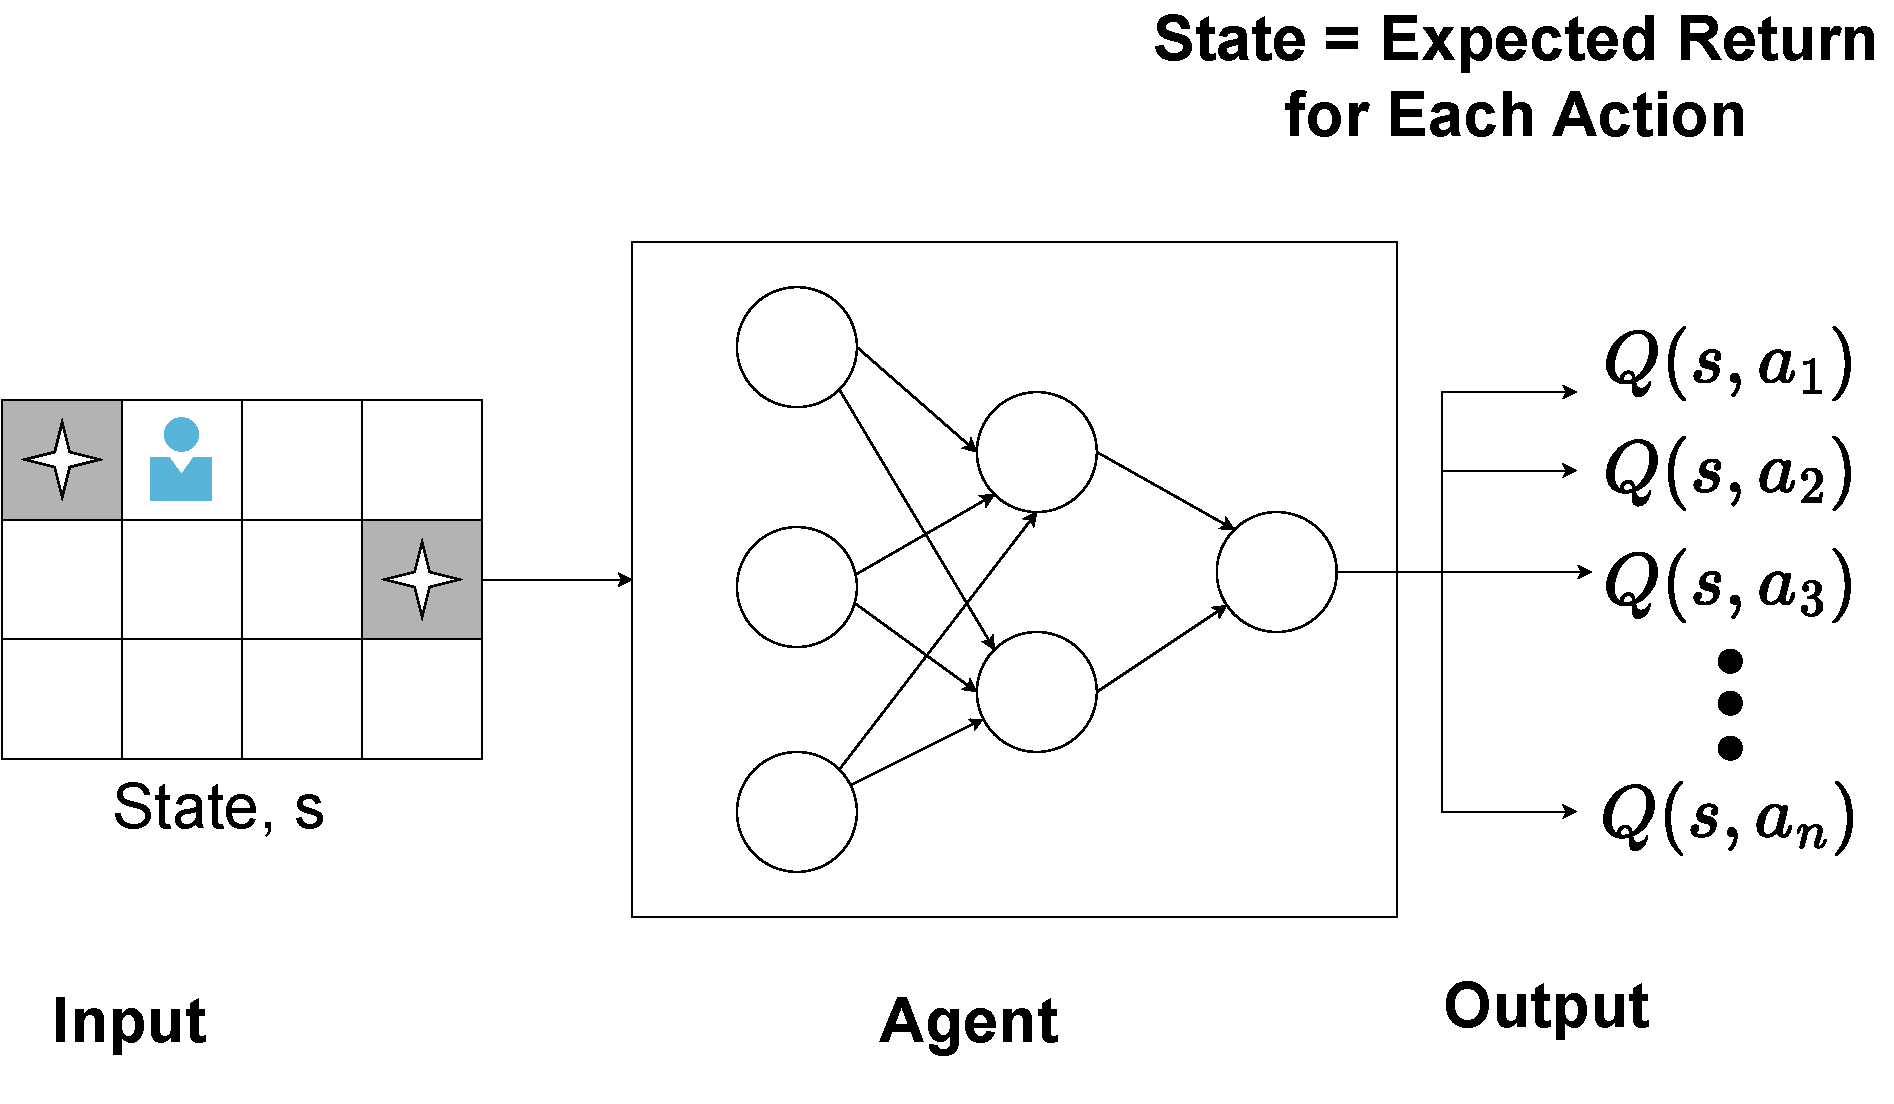
\includegraphics[width=0.80\textwidth]{figures/QLearning2.pdf}
\column{.30\textwidth} 

\vspace{10pt}

That can serve as a ground truth to the agent.

    \end{columns}

\end{frame}

%---------------------------------------------

\begin{frame}{Q-Learning}
\begin{columns}[c]
    \column{.65\textwidth} 
    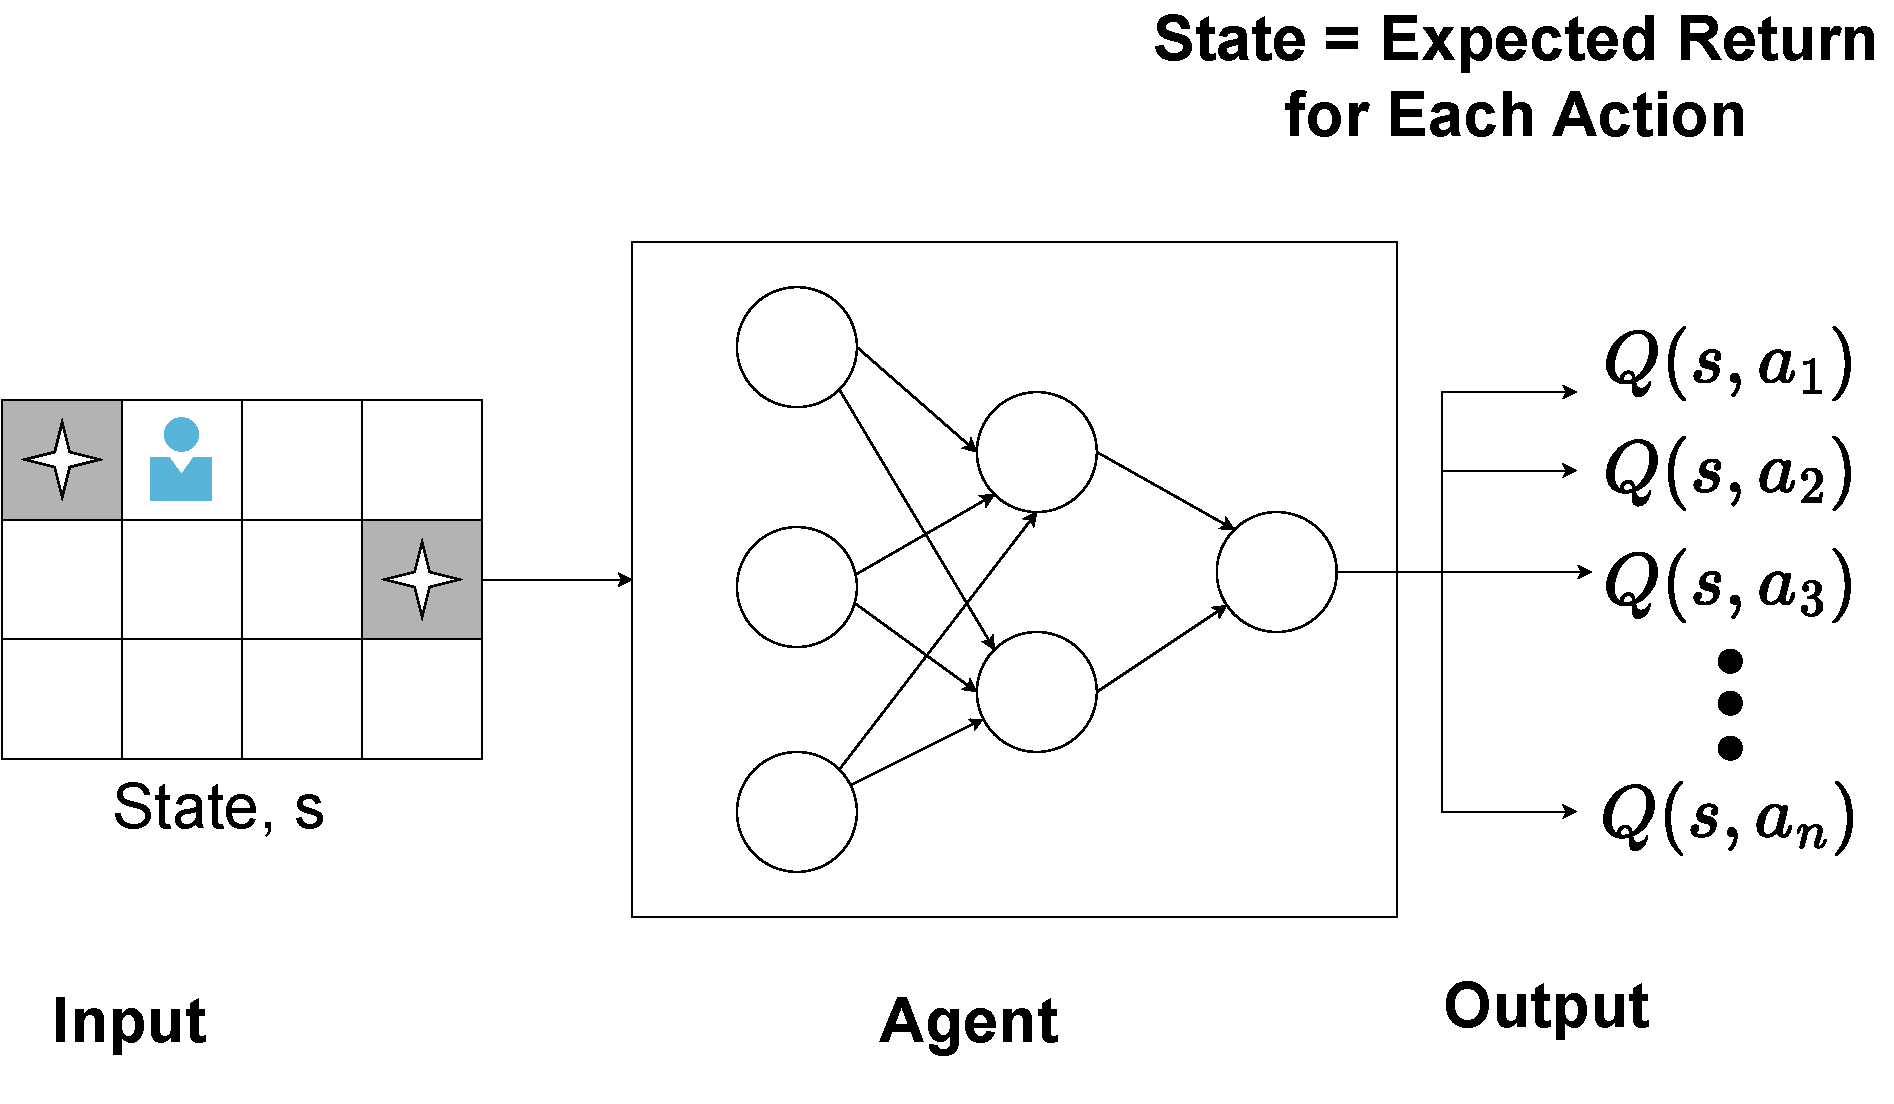
\includegraphics[width=0.80\textwidth]{figures/QLearning2.pdf}
\column{.35\textwidth} 

Maximize target return $\to$ train the agent.

\end{columns}

\end{frame}

%---------------------------------------------

\begin{frame}{Q-Learning}
\begin{columns}[c]
    \column{.65\textwidth} 
    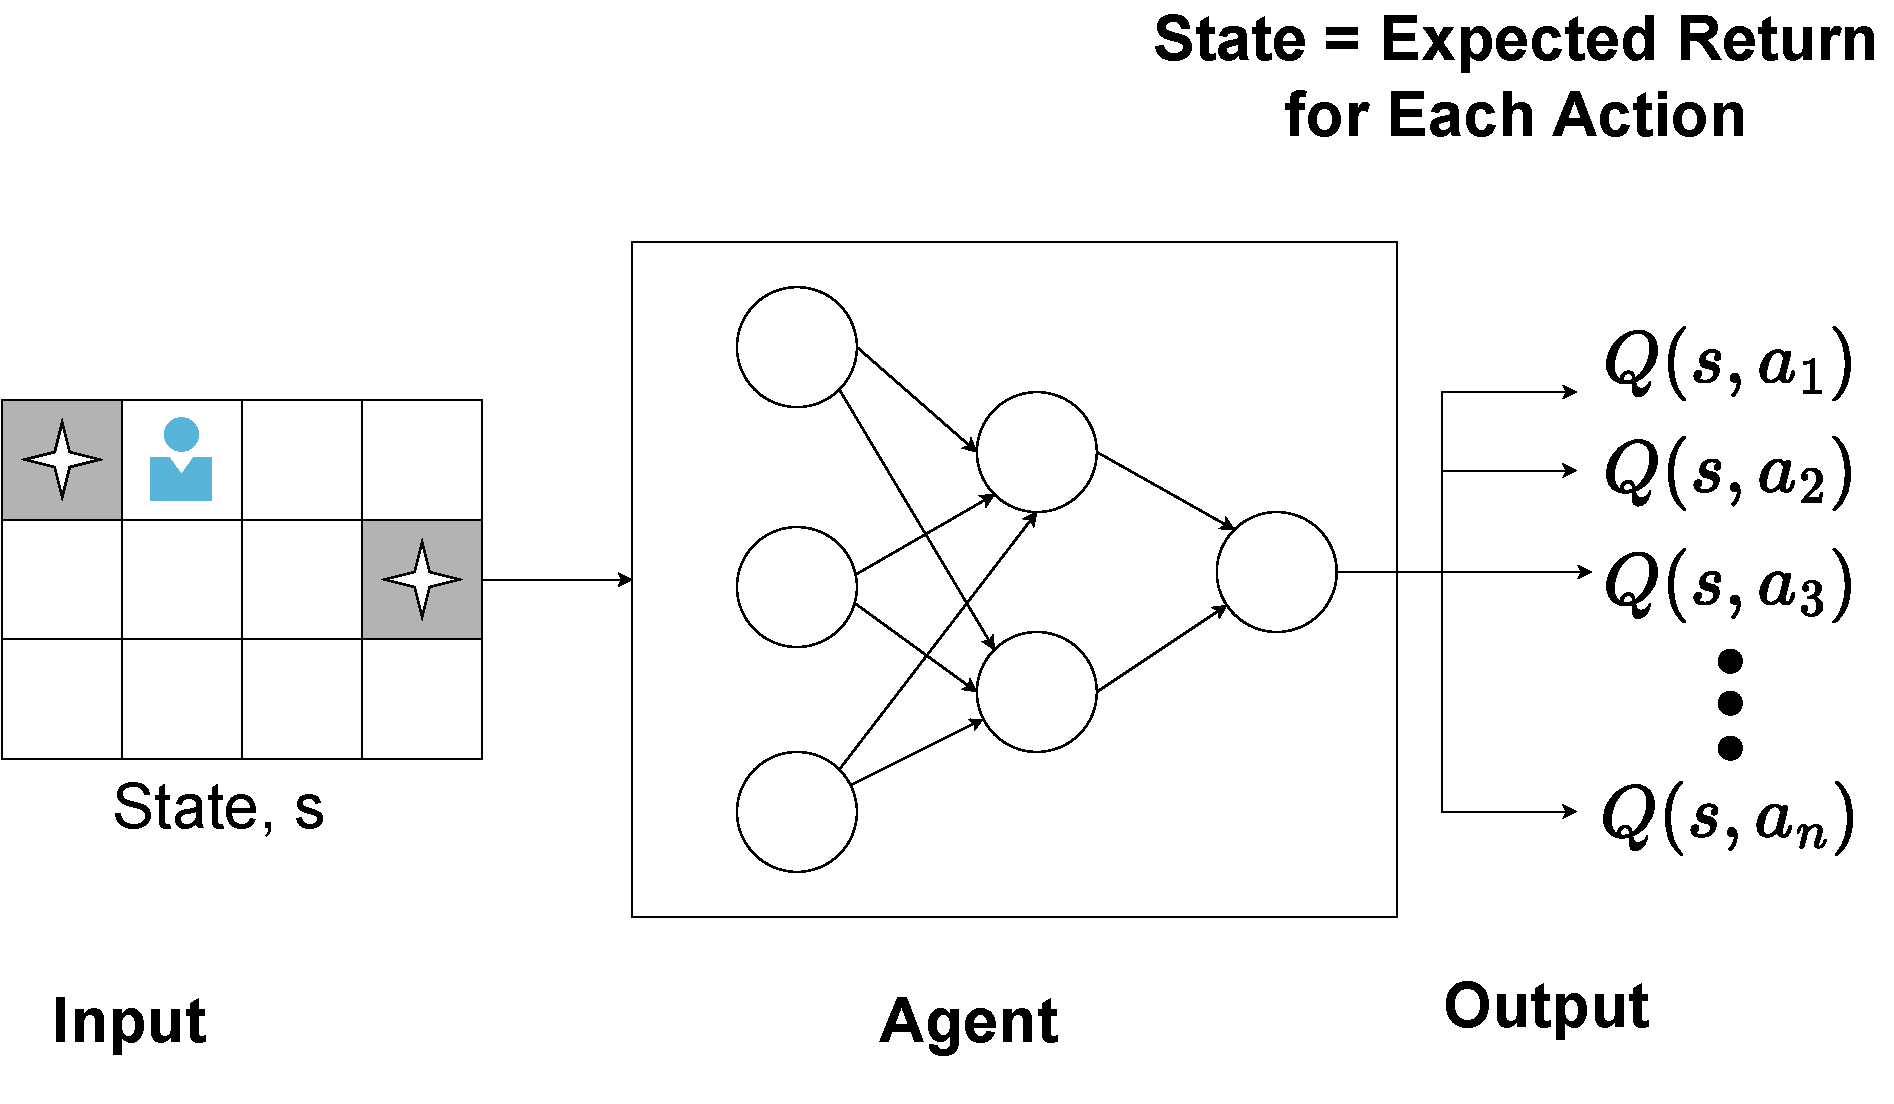
\includegraphics[width=0.80\textwidth]{figures/QLearning2.pdf}
\column{.35\textwidth} 

\vspace{10pt}

To do this, we want to formulate a loss function that will essentially return an expected return if we were able to take all of the best actions.


\end{columns}

\end{frame}

%---------------------------------------------

\begin{frame}{Q-Learning}
\begin{columns}[c]
    \column{.65\textwidth} 
    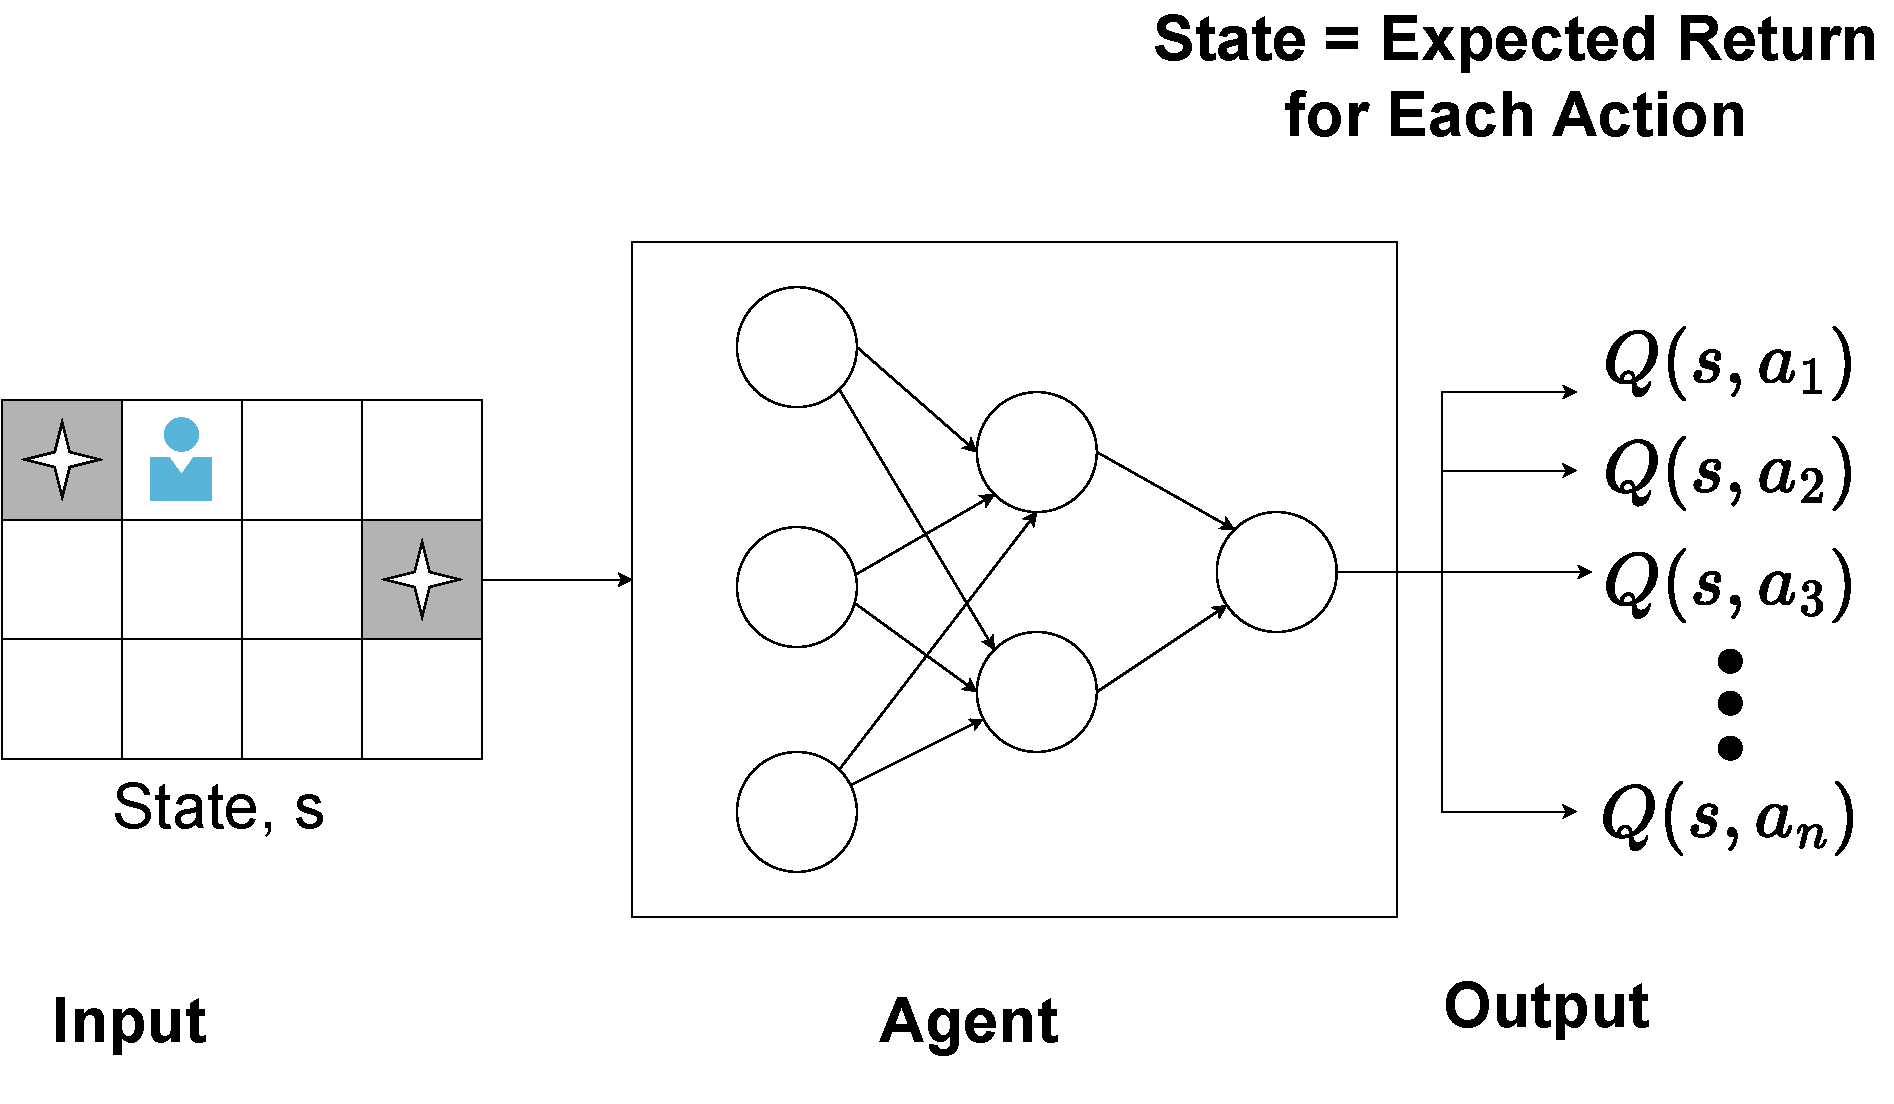
\includegraphics[width=0.80\textwidth]{figures/QLearning2.pdf}
\column{.35\textwidth} 

\vspace{10pt}

Essentially, in this case, the target is 
$$
r + \gamma \max_{a_{t+1}}Q(s_{t+1}, a_{t+1})
$$

    \end{columns}


\end{frame}


%---------------------------------------------

\begin{frame}{Q-Learning}
\begin{columns}[c]
    \column{.65\textwidth} 
    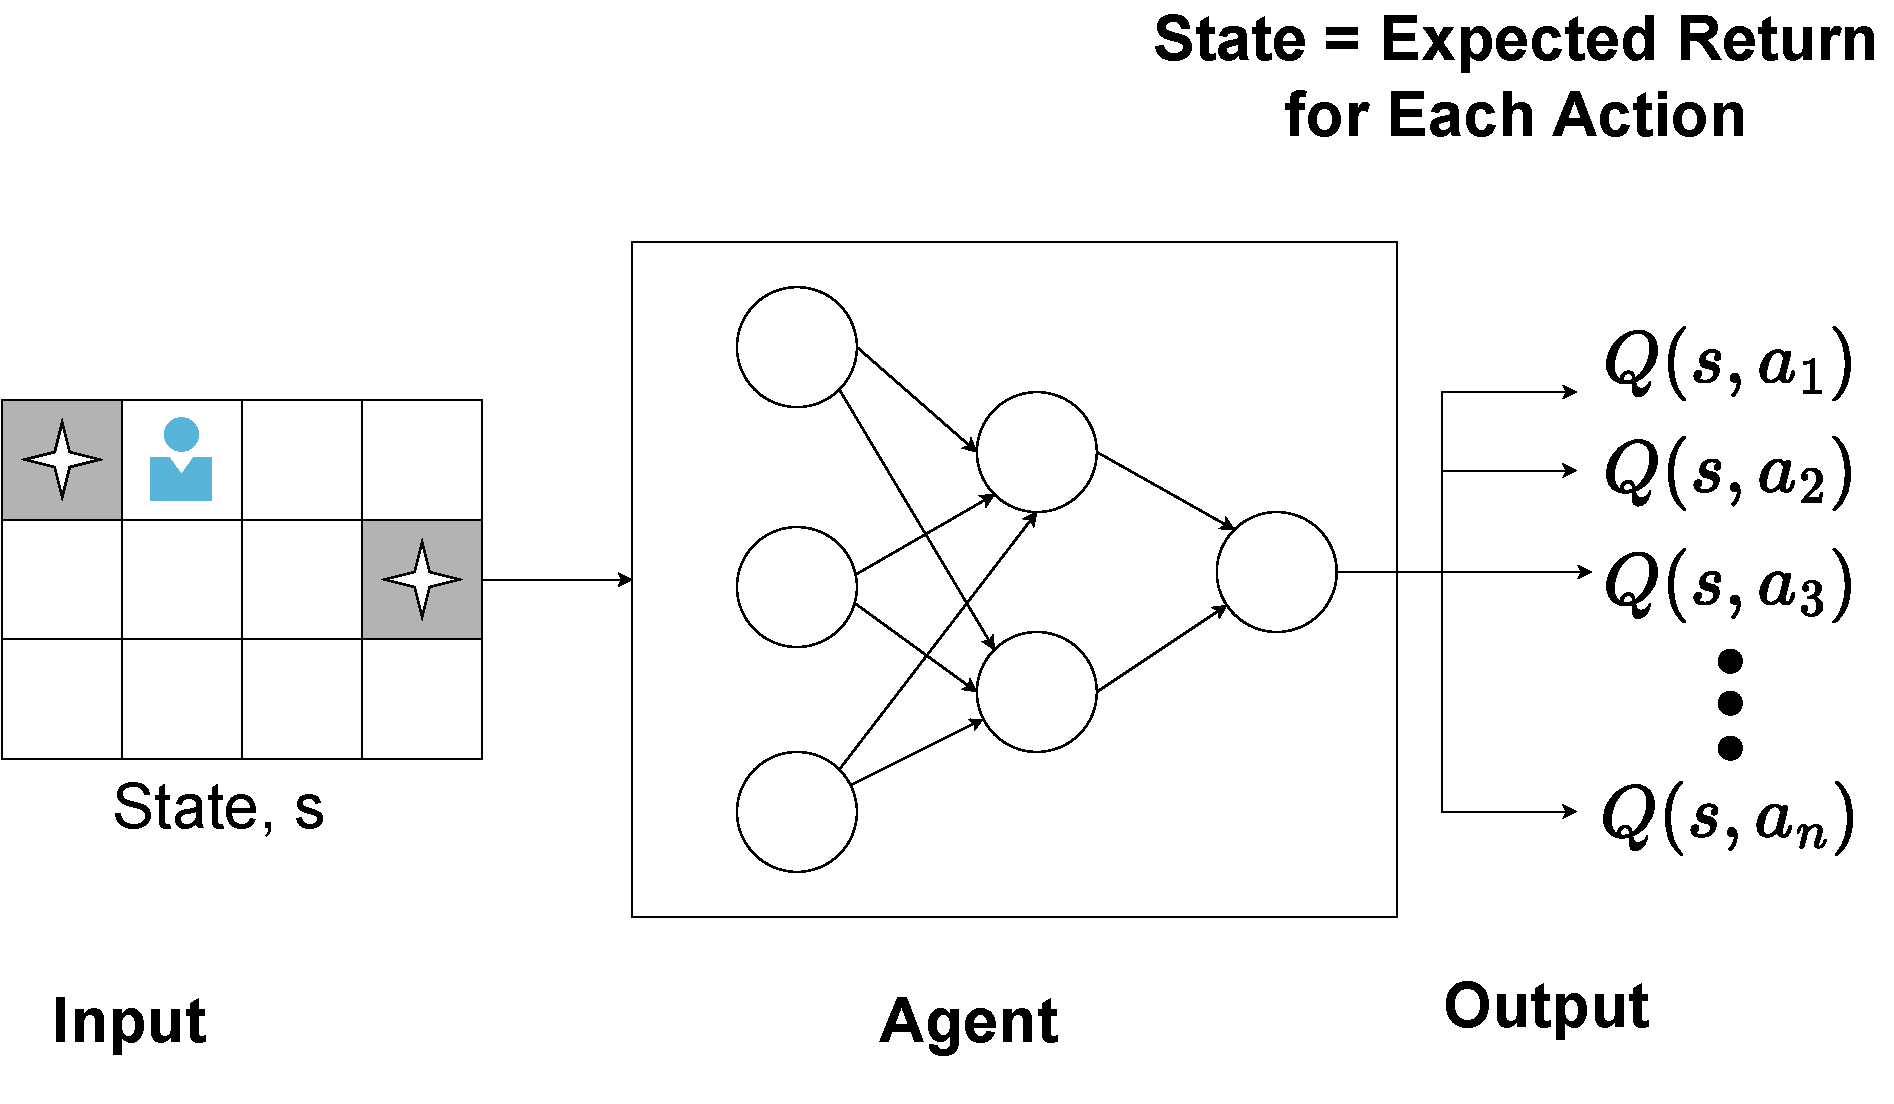
\includegraphics[width=0.80\textwidth]{figures/QLearning2.pdf}
\column{.35\textwidth} 

And, the predicted variable would denoted by $Q(s, a)$.


\end{columns}


\end{frame}

\begin{frame}{Q-Learning}
    \begin{columns}[c]
        \column{.65\textwidth} 
        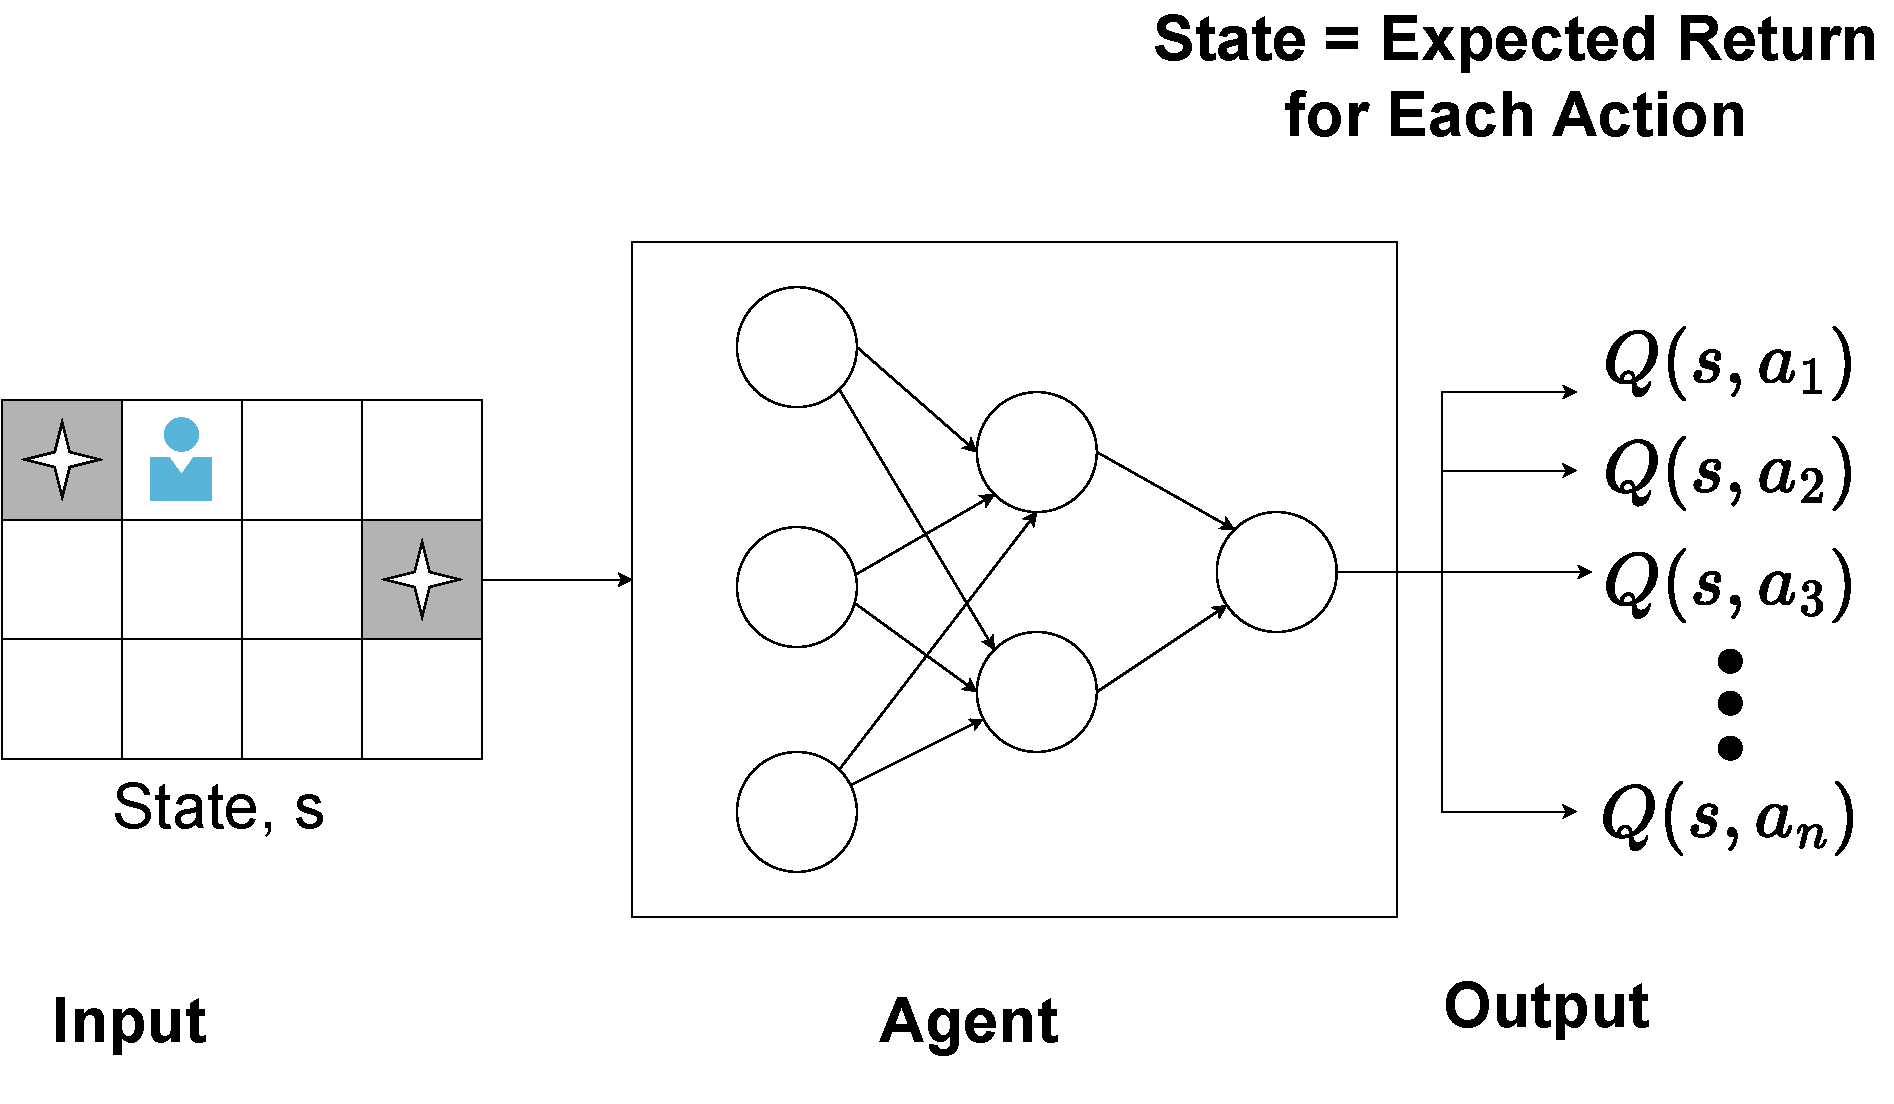
\includegraphics[width=0.80\textwidth]{figures/QLearning2.pdf}
    \column{.35\textwidth} 
    
    And, the predicted variable would denoted by $Q(s, a)$.
    
    
    \end{columns}
    
    
    Then, we can define Q-loss as 
    $$
    \Lcal = \Ebb \bigg[ \bigg|\bigg| \bigg( r + \gamma \max_{a_{t+1}}Q(s_{t+1}, a_{t+1})
    \bigg) - Q(s, a) \bigg|\bigg|  ^2 \bigg]
    $$
    
\end{frame}
    

%---------------------------------------------

\begin{frame}{Q-Learning}

\begin{center}
    Using NN, we can learn the Q-function and then infer the optimal policy $\pi(s) $ using $\pi(s) = \argmax_a Q(s, a)$.
\end{center}


\end{frame}

%---------------------------------------------

\begin{frame}{Q-Learning}

\begin{center}
    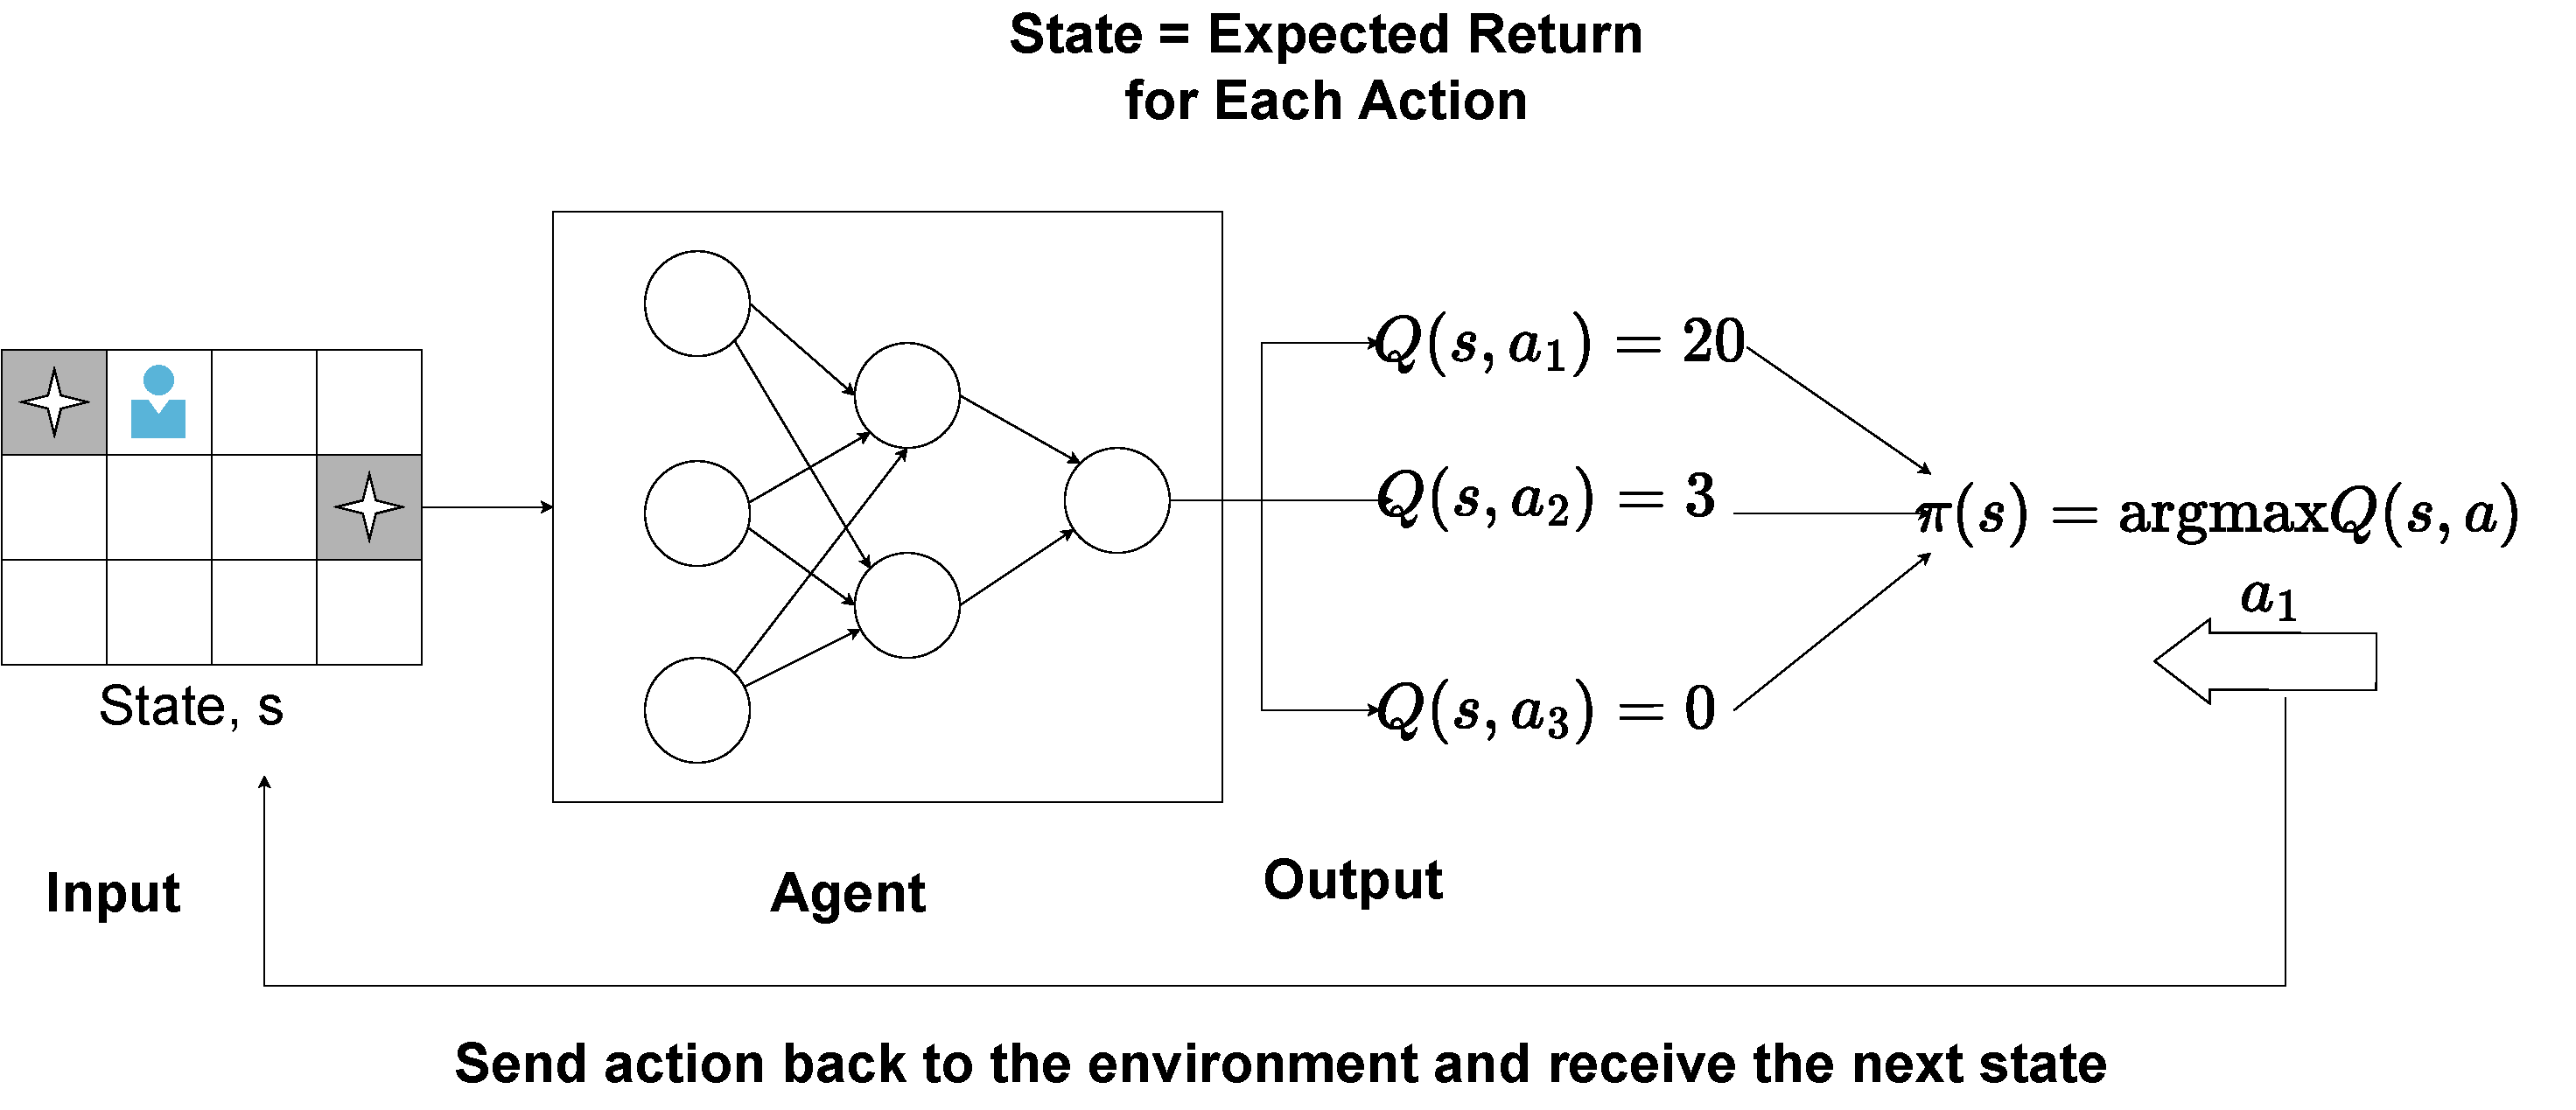
\includegraphics[width=0.80\textwidth]{figures/QLearning3.pdf}
\end{center}


\end{frame}

%---------------------------------------------


\begin{frame}{Solving Optimal Policy}

    \small

Assuming that the neural network will be parametrized by $\theta$ (i.e function weights, the thing we want to keep updating in backward propagation), 

\vspace{4pt}

\textbf{Forward propagation:}

$$\Lcal(\theta_i) = \Ebb \bigg[ \bigg|\bigg| \bigg( r + \gamma \max_{a_{t+1}}Q(s_{t+1}, a_{t+1},\theta_{i-1})
\bigg) - Q(s, a, \theta_i) \bigg|\bigg|  ^2 \bigg]$$

Iteratively make $Q(s, a, \theta_i)$ close to the target (the first time in the squared difference above).

\vspace{4pt}

\textbf{Backward propagation:}

$$
\nabla_{\theta_i}\Lcal(\theta_i) 
\Ebb \bigg[ \bigg( r + \gamma \max_{a_{t+1}}Q(s_{t+1}, a_{t+1},\theta_{i-1})
\bigg) - Q(s, a, \theta_i)  \nabla_{\theta_i}Q(s, a, \theta_i) \bigg]$$
\end{frame}

%---------------------------------------------
\begin{frame}{Case Study: Atari Breakout Game}
    \begin{center}
    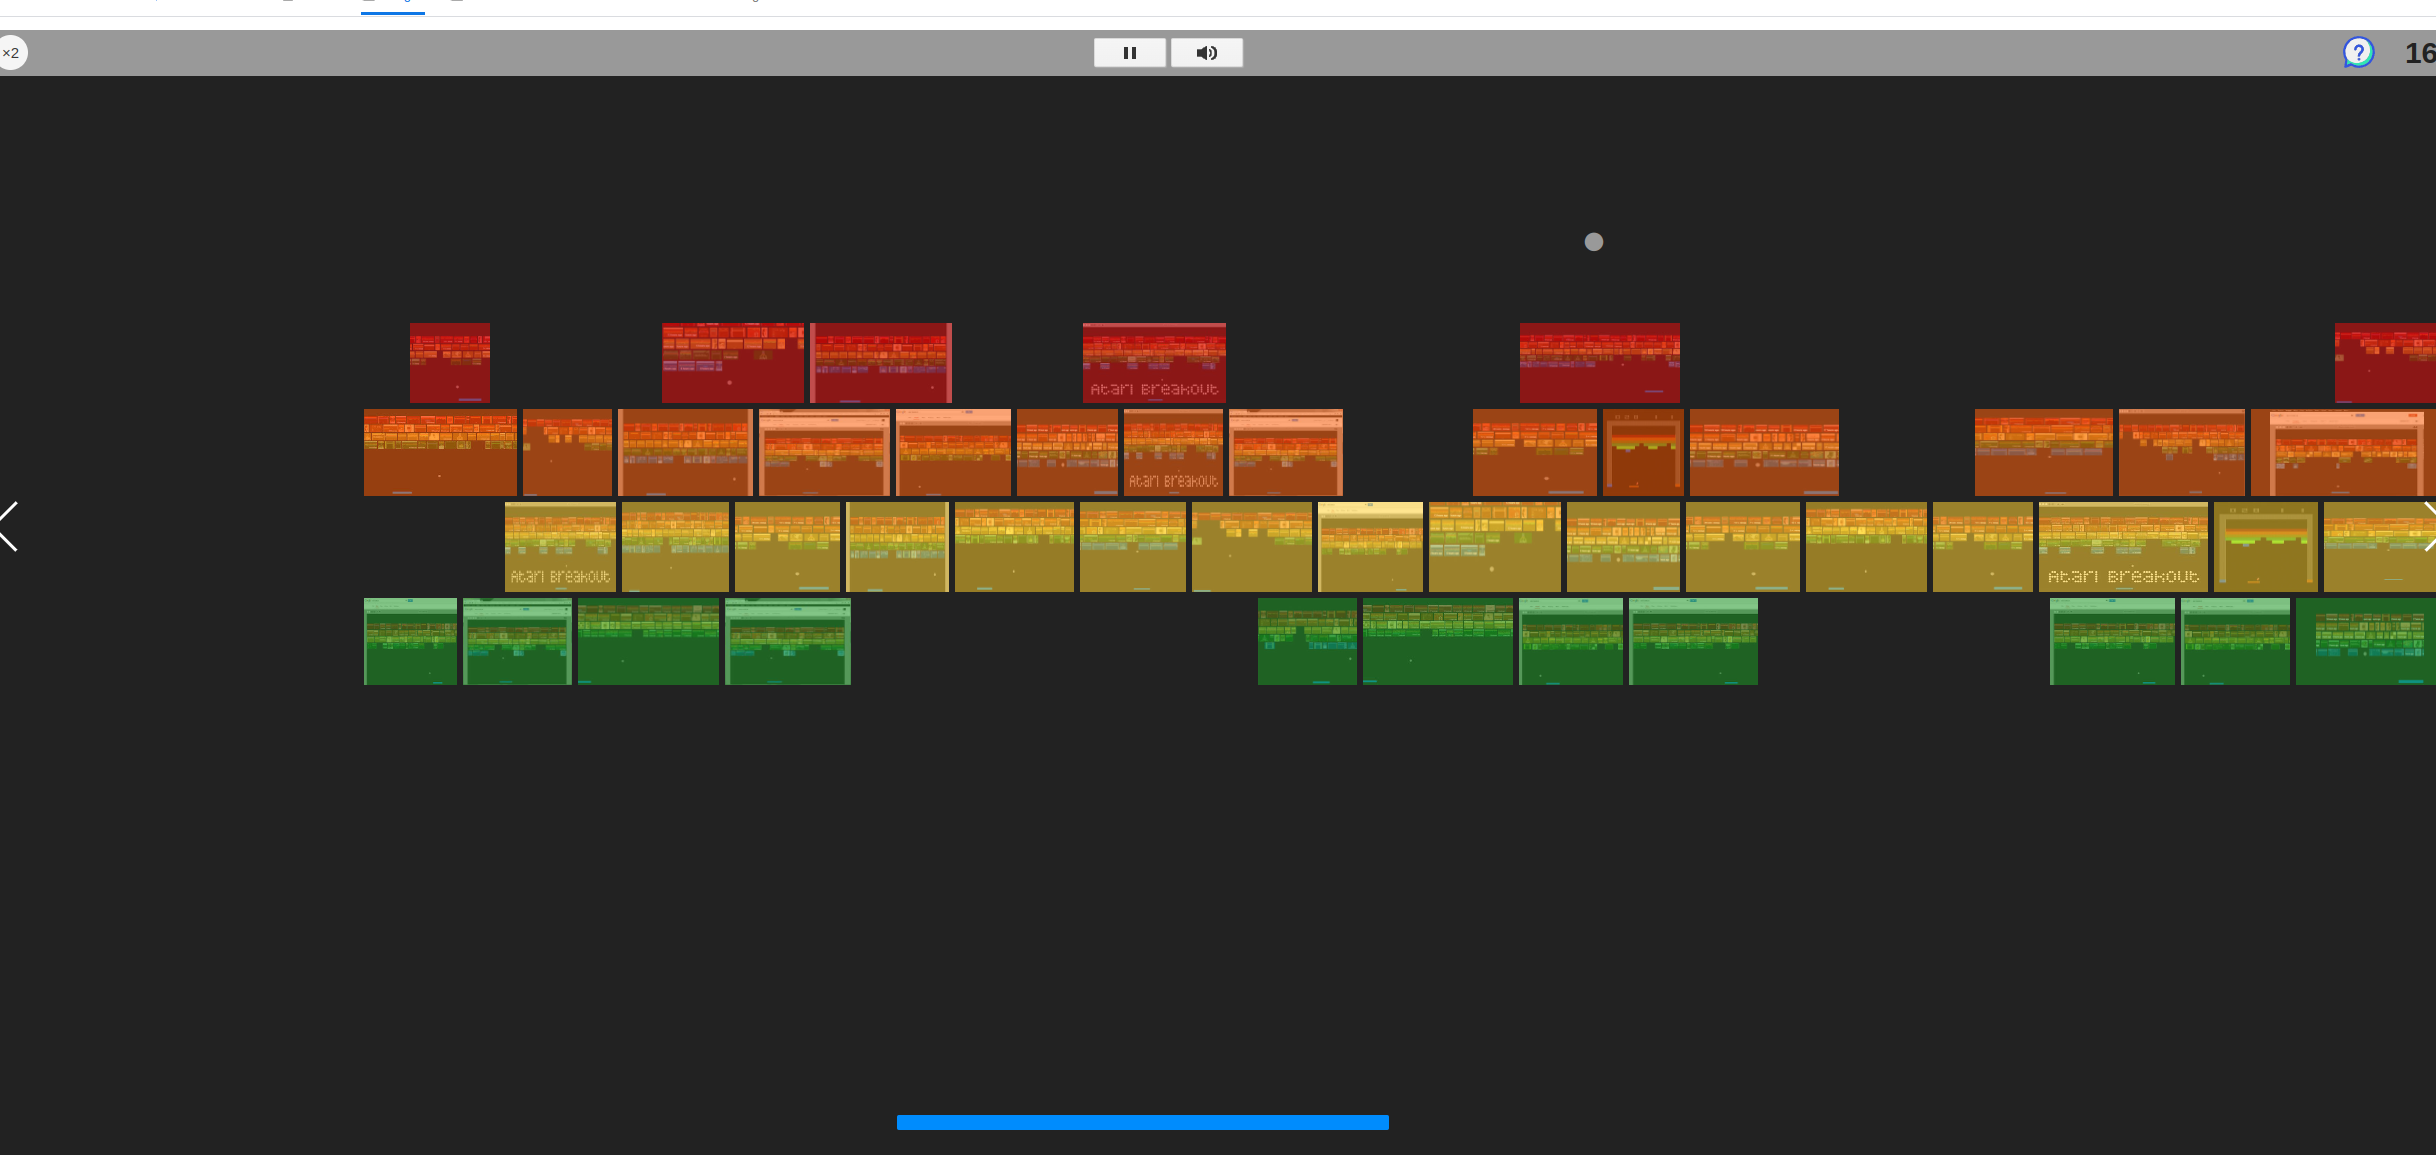
\includegraphics[width=0.80\textwidth]{figures/atari_breakout.png}
\end{center}
\end{frame}

%---------------------------------------------
\begin{frame}{Case Study: Atari Breakout Game}
    \begin{center}
    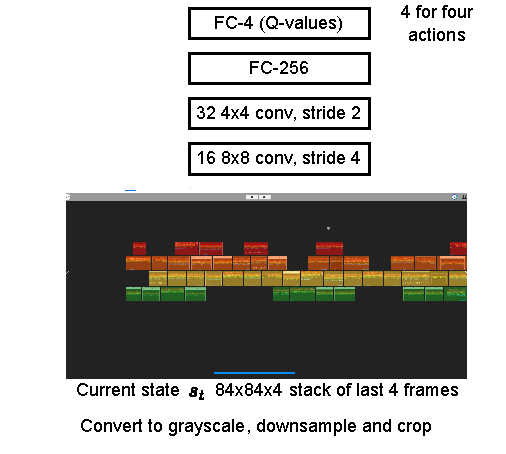
\includegraphics[width=0.45\textwidth]{figures/Atari_Net.pdf}
\end{center}
\end{frame}

%---------------------------------------------
\begin{frame}{Training the Q-network: Experience Replay}

    \begin{tblock}{}
    Learning from batches of consecutive samples is problematic:
    \begin{itemize}
        \item Samples are correlated $\to$ inefficient learning.
        \item Current Q-network parameters determine the next training samples (e.g. if maximizing
action is to move left, training samples will be dominated by samples from left-hand size) $\to$  can lead to bad feedback loops.
    \end{itemize}
    \end{tblock}
\end{frame}

%---------------------------------------------
\begin{frame}{Training the Q-network: Experience Replay}

    \begin{tblock}{}
    We address these problems using \textbf{experience replay}:
    \begin{itemize}
        \item Continually update a replay memory table of transitions ($s_t$, $a_t$, $r_t$, $s_{t+1}$) as game (experience) episodes are played
        \item Train Q-network on random mini-batches of transitions from the replay memory, instead of consecutive samples
        \item Each transition can also contribute to multiple weight updates
    \end{itemize}
    \end{tblock}

    \small 
    From [Mnih et al. NIPS Workshop 2013; Nature 2015]
    
    \vspace{10pt}
    Original paper: \url{https://arxiv.org/pdf/1312.5602.pdf}
\end{frame}


%---------------------------------------------
\begin{frame}{Experience Replay Algorithm}


\begin{center}
\begin{tikzpicture}
    \node[anchor=south west,inner sep=0] (image) at (0,0) {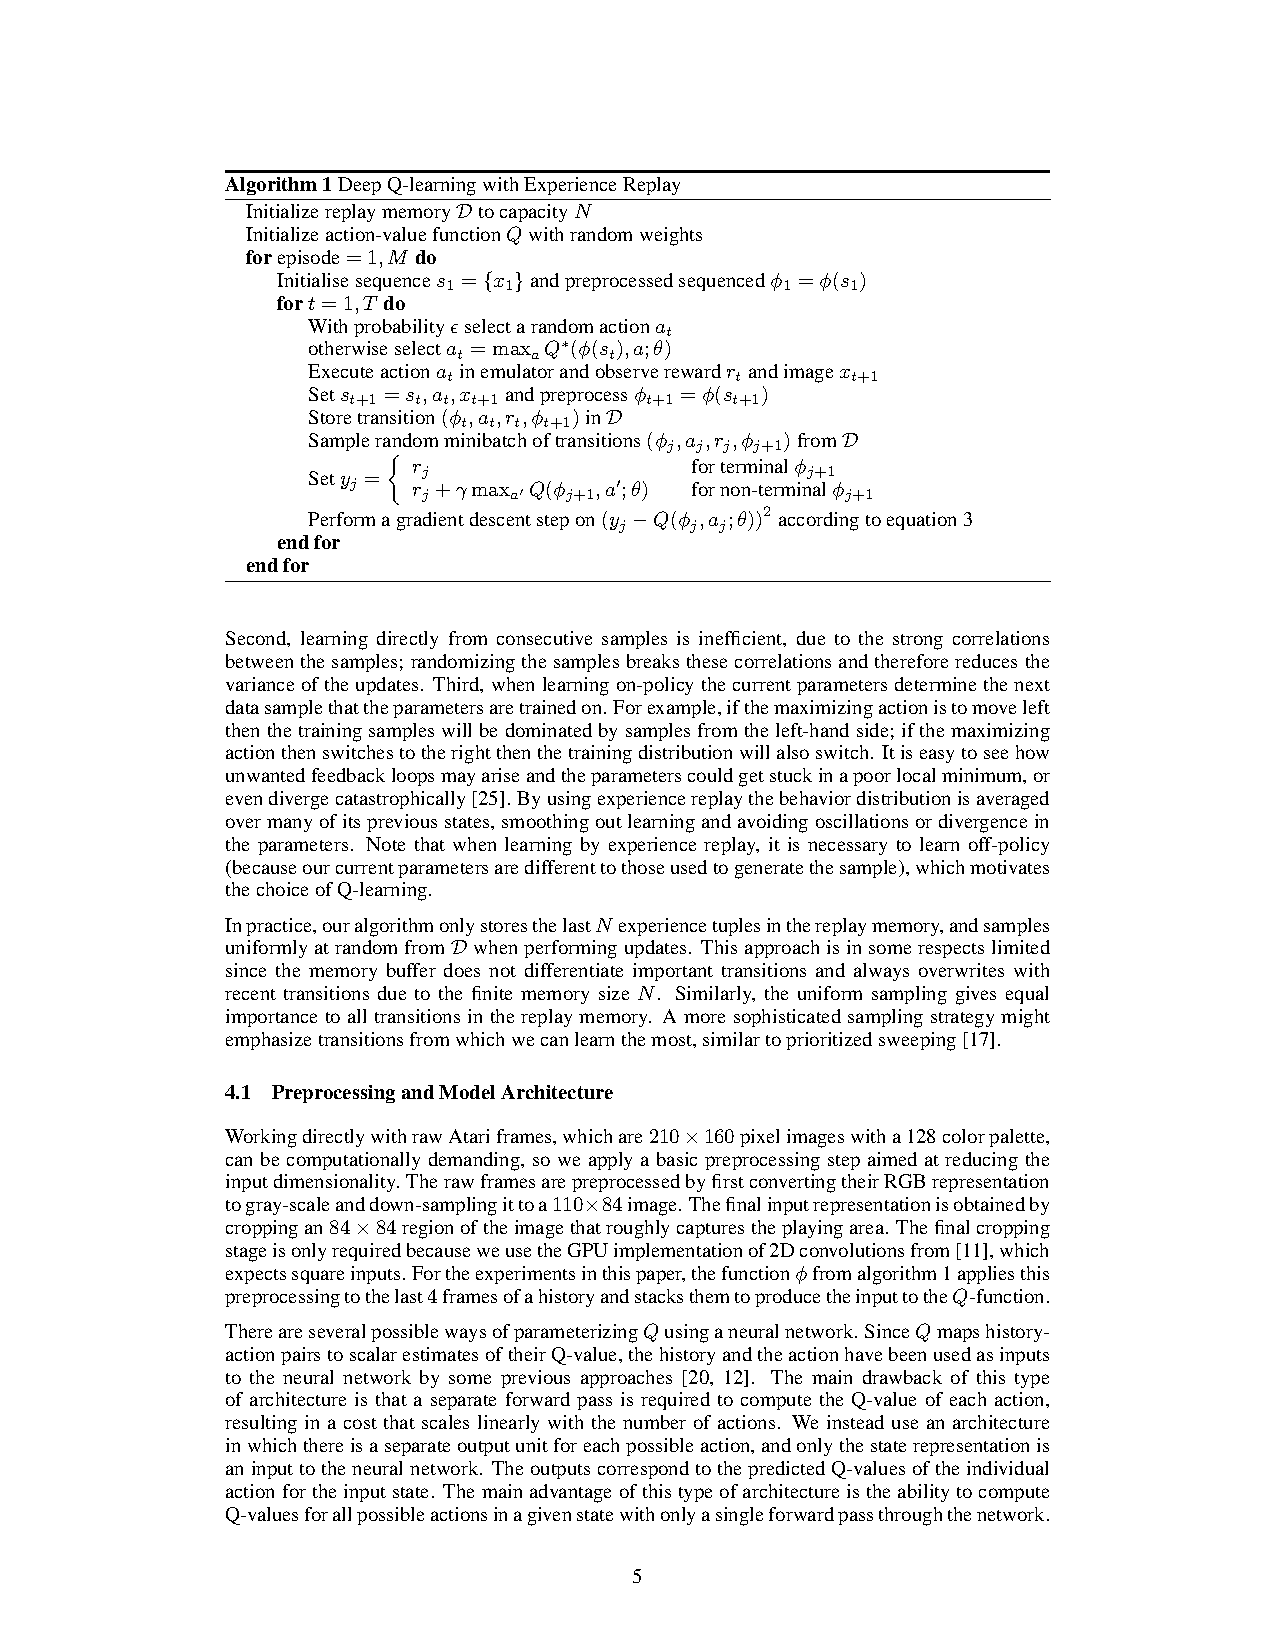
\includegraphics[width=0.99\textwidth, trim={60 500 60 60}, clip]{figures/Experience_Replay.pdf}};
    \begin{scope}[x={(image.south east)},y={(image.north west)}]
        \draw[blue,thick,rounded corners] (0.6,0.70) rectangle (0.1,0.75); % Draw the blue box
        \draw[->, ultra thick, blue] (0.6,0.72) -- (0.70,0.72); % Draw the blue arrow
        \node[blue] at (0.88,0.72) {Play M episodes (full games)}; % Add the blue text
    \end{scope}
\end{tikzpicture}
\end{center}
\end{frame}

%---------------------------------------------
\begin{frame}{Experience Replay Algorithm}
\begin{center}
\begin{tikzpicture}
    \node[anchor=south west,inner sep=0] (image) at (0,0) {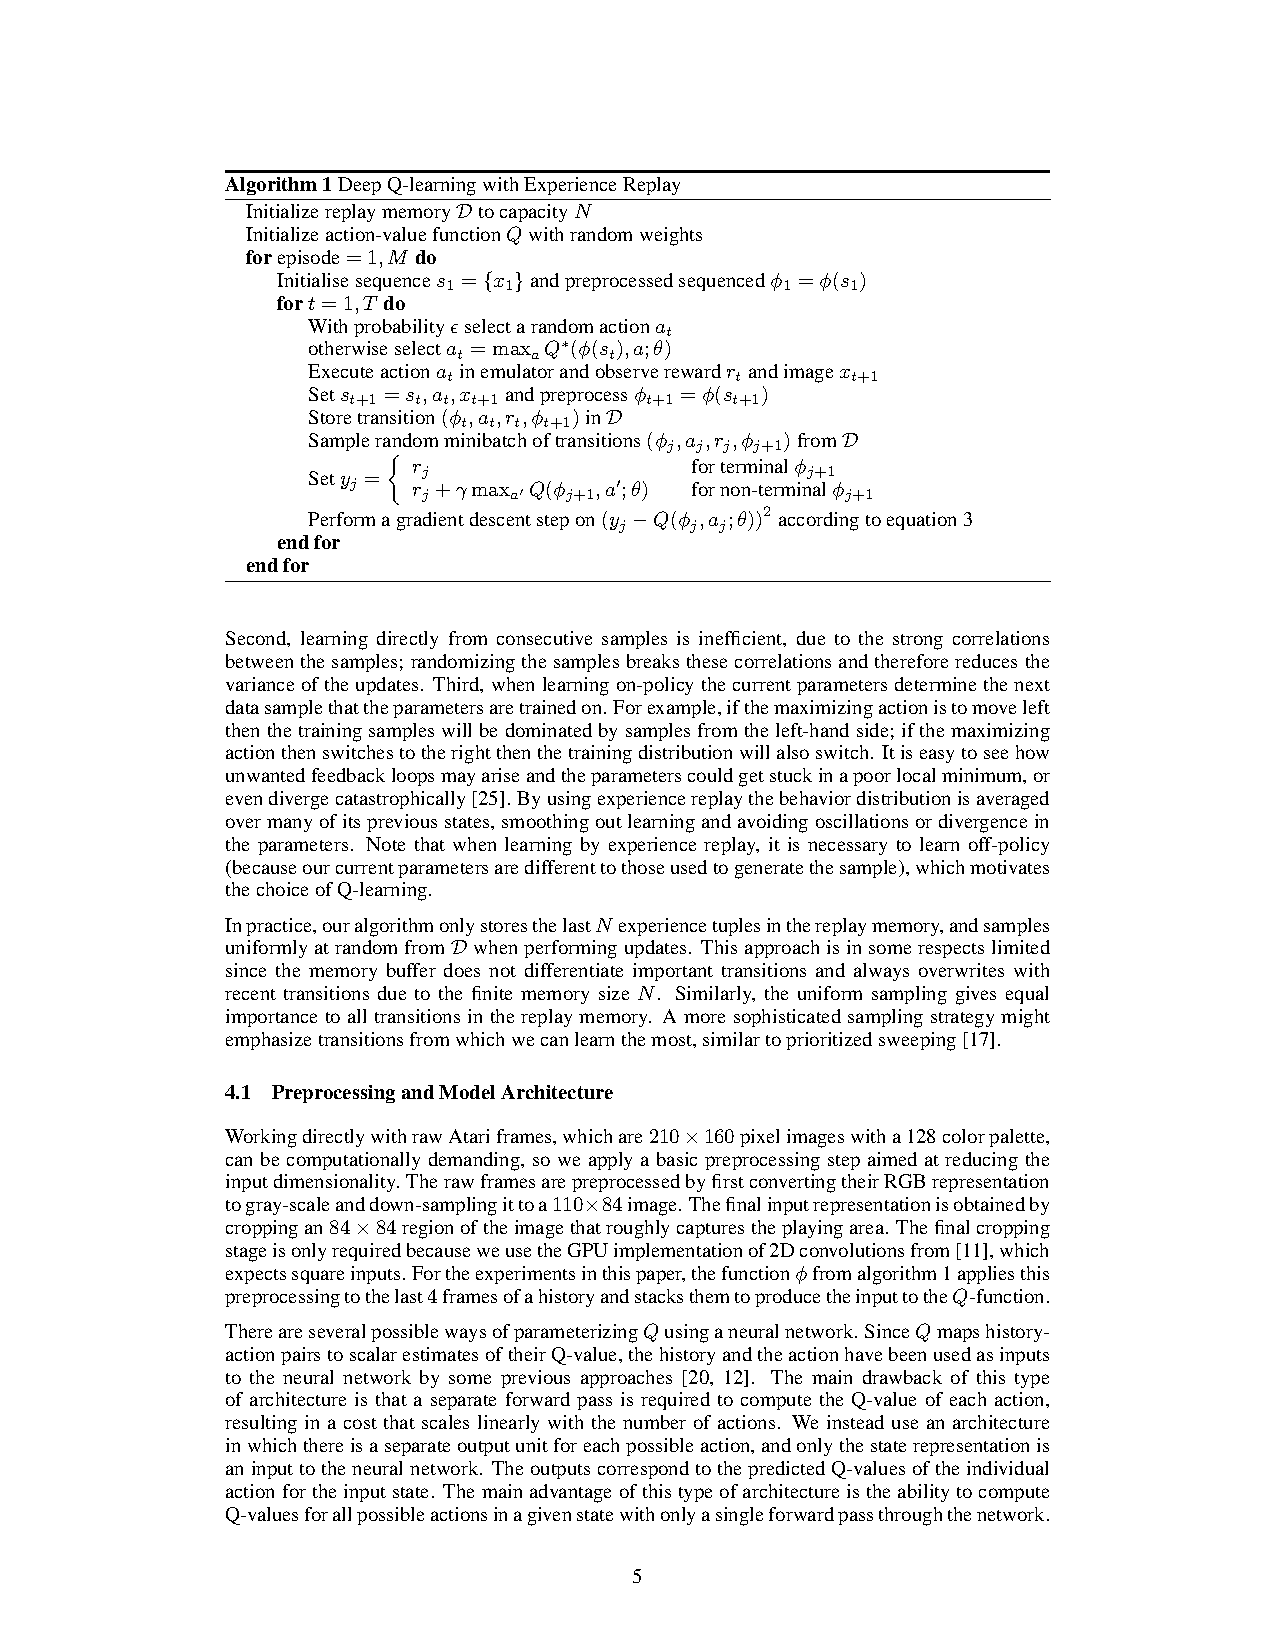
\includegraphics[width=0.99\textwidth, trim={60 500 60 60}, clip]{figures/Experience_Replay.pdf}};
    \begin{scope}[x={(image.south east)},y={(image.north west)}]
        \draw[blue,thick,rounded corners] (0.6,0.65) rectangle (0.1,0.70); % Draw the blue box
        % \draw[->, ultra thick, blue] (0.6,0.72) -- (0.70,0.72); % Draw the blue arrow
        \node[blue, font=\footnotesize] at (0.85,0.62) {Initialize state (starting game screen pixels)}; % Add the blue text
\node[blue, font=\footnotesize] at (0.85,0.58) { at the beginning of each episode};
    \end{scope}
\end{tikzpicture}
\end{center}
\end{frame}

%---------------------------------------------
\begin{frame}{Experience Replay Algorithm}
\begin{center}
\begin{tikzpicture}
    \node[anchor=south west,inner sep=0] (image) at (0,0) {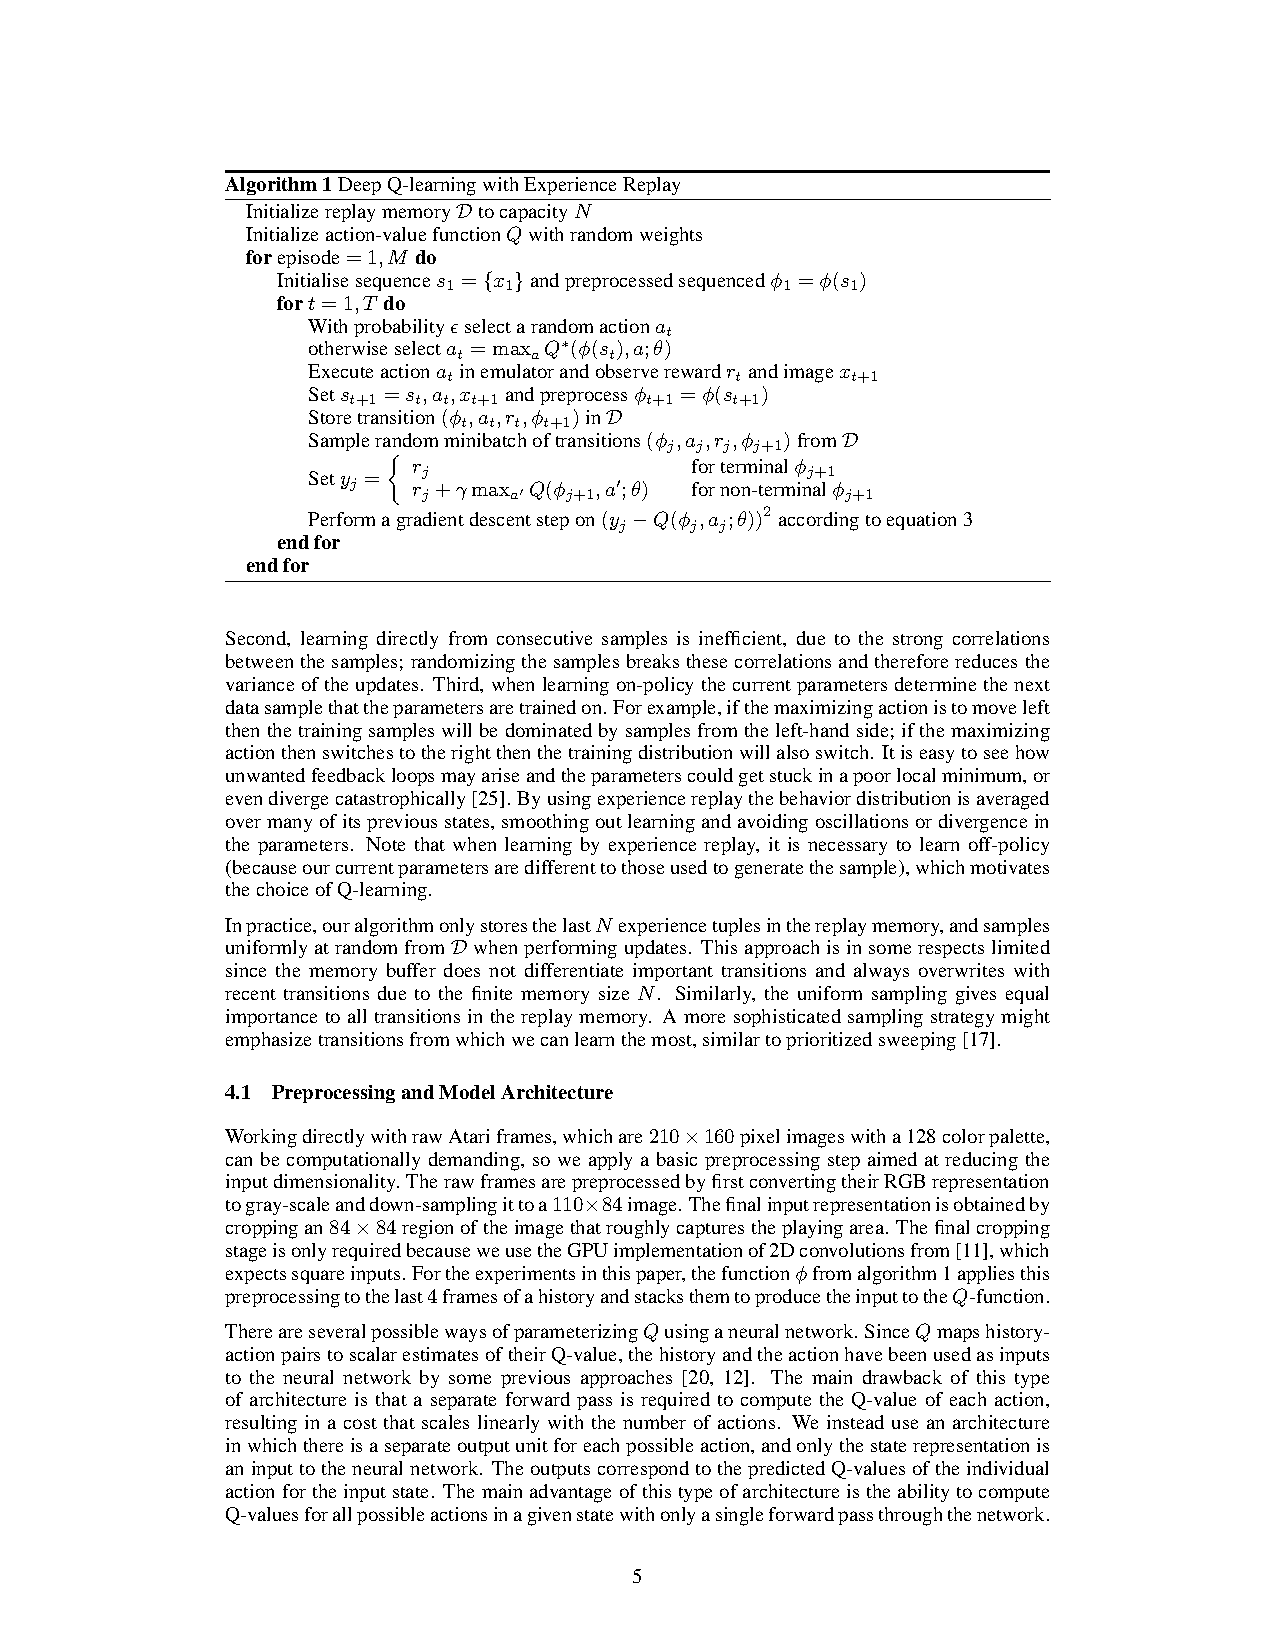
\includegraphics[width=0.99\textwidth, trim={60 500 60 60}, clip]{figures/Experience_Replay.pdf}};
    \begin{scope}[x={(image.south east)},y={(image.north west)}]
        \draw[blue,thick,rounded corners] (0.6,0.60) rectangle (0.1,0.65); % Draw the blue box
        % \draw[->, ultra thick, blue] (0.6,0.72) -- (0.70,0.72); % Draw the blue arrow
        \node[blue, font=\footnotesize] at (0.85,0.62) {For each timestep $t$ of the game}; % Add the blue text
    \end{scope}
\end{tikzpicture}
\end{center}
\end{frame}

%---------------------------------------------
\begin{frame}{Experience Replay Algorithm}
\begin{center}
\begin{tikzpicture}
    \node[anchor=south west,inner sep=0] (image) at (0,0) {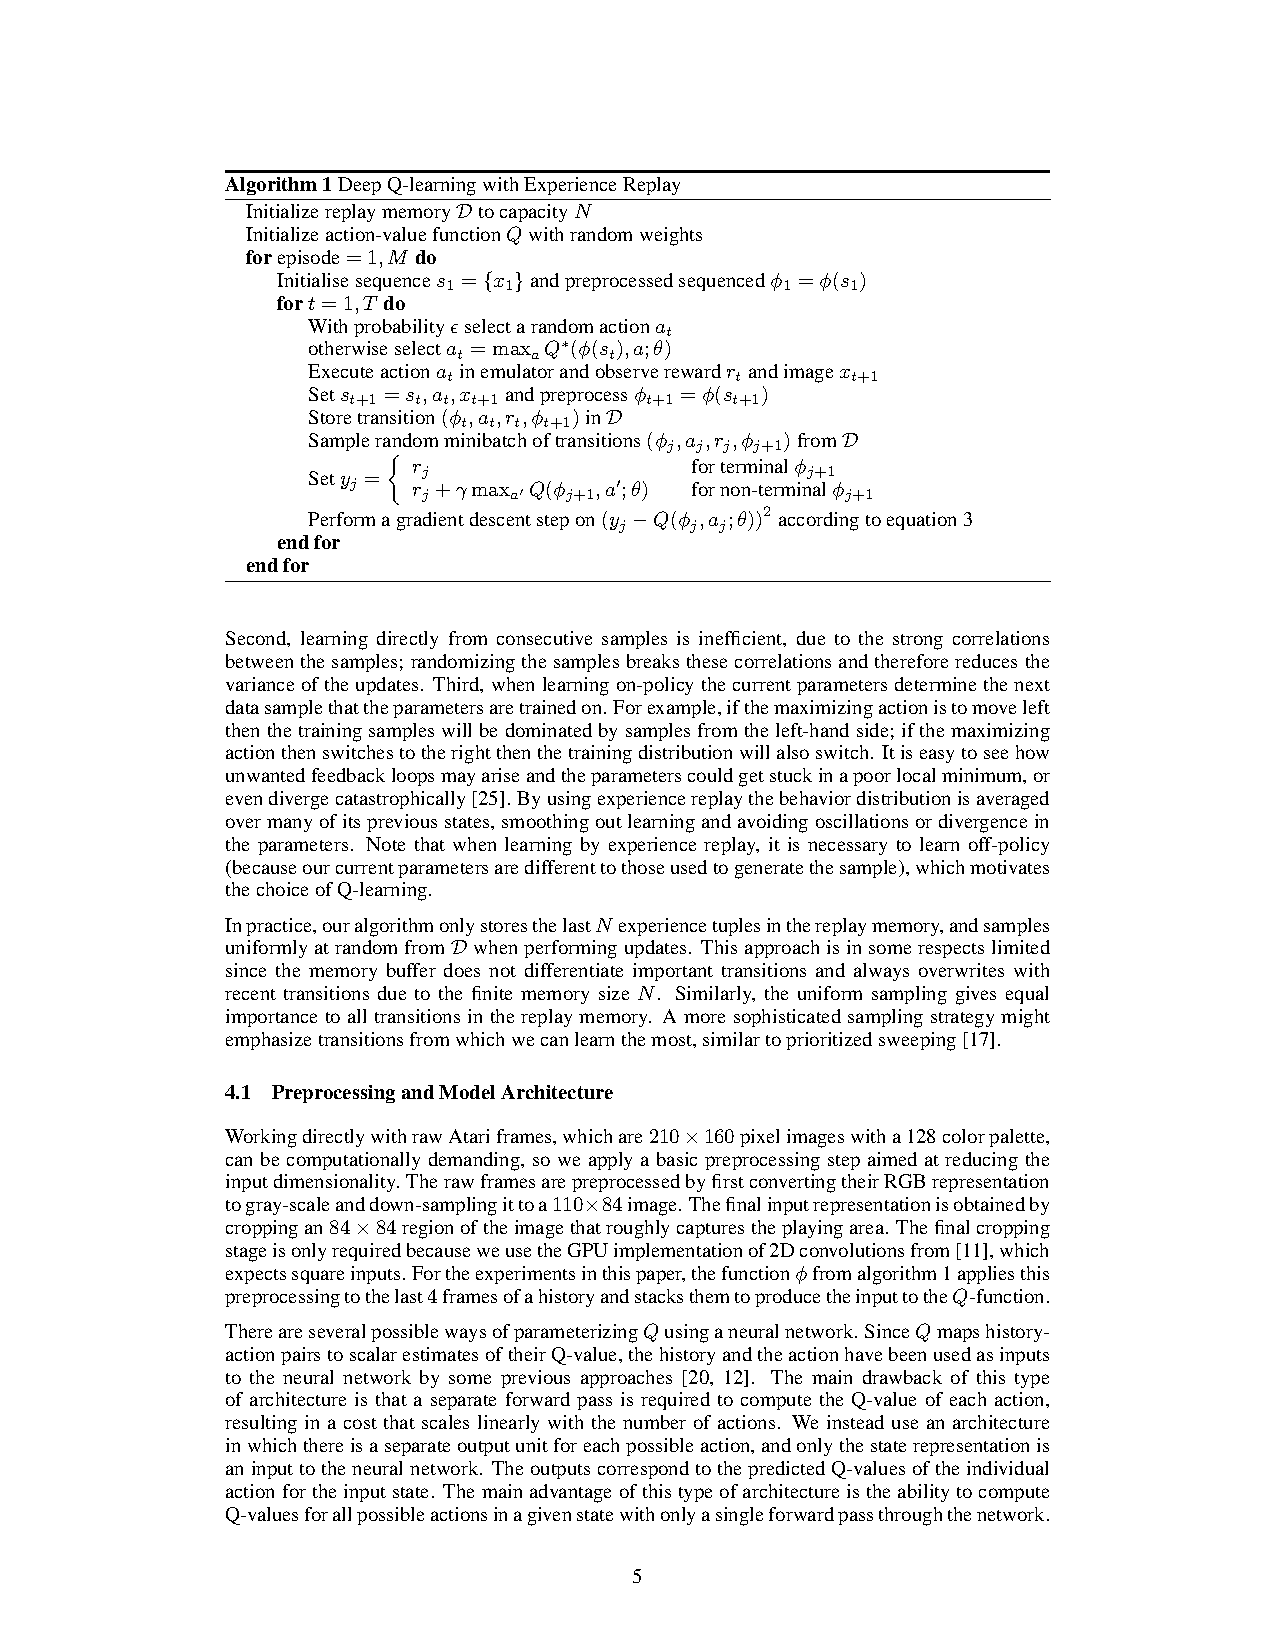
\includegraphics[width=0.99\textwidth, trim={60 500 60 60}, clip]{figures/Experience_Replay.pdf}};
    \begin{scope}[x={(image.south east)},y={(image.north west)}]
        \draw[blue,thick,rounded corners] (0.6,0.50) rectangle (0.1,0.60); % Draw the blue box
        % \draw[->, ultra thick, blue] (0.6,0.72) -- (0.70,0.72); % Draw the blue arrow
        \node[draw, text width=3cm, align=center, blue, font=\footnotesize] at (0.85,0.50) {With small probability,\\
select a random \\
action (explore), \\
otherwise, select \\
greedy action from \\
current policy}; % Add the blue text box
    \end{scope}
\end{tikzpicture}
\end{center}
\end{frame}


%---------------------------------------------
\begin{frame}{Experience Replay Algorithm}
\begin{center}
\begin{tikzpicture}
    \node[anchor=south west,inner sep=0] (image) at (0,0) {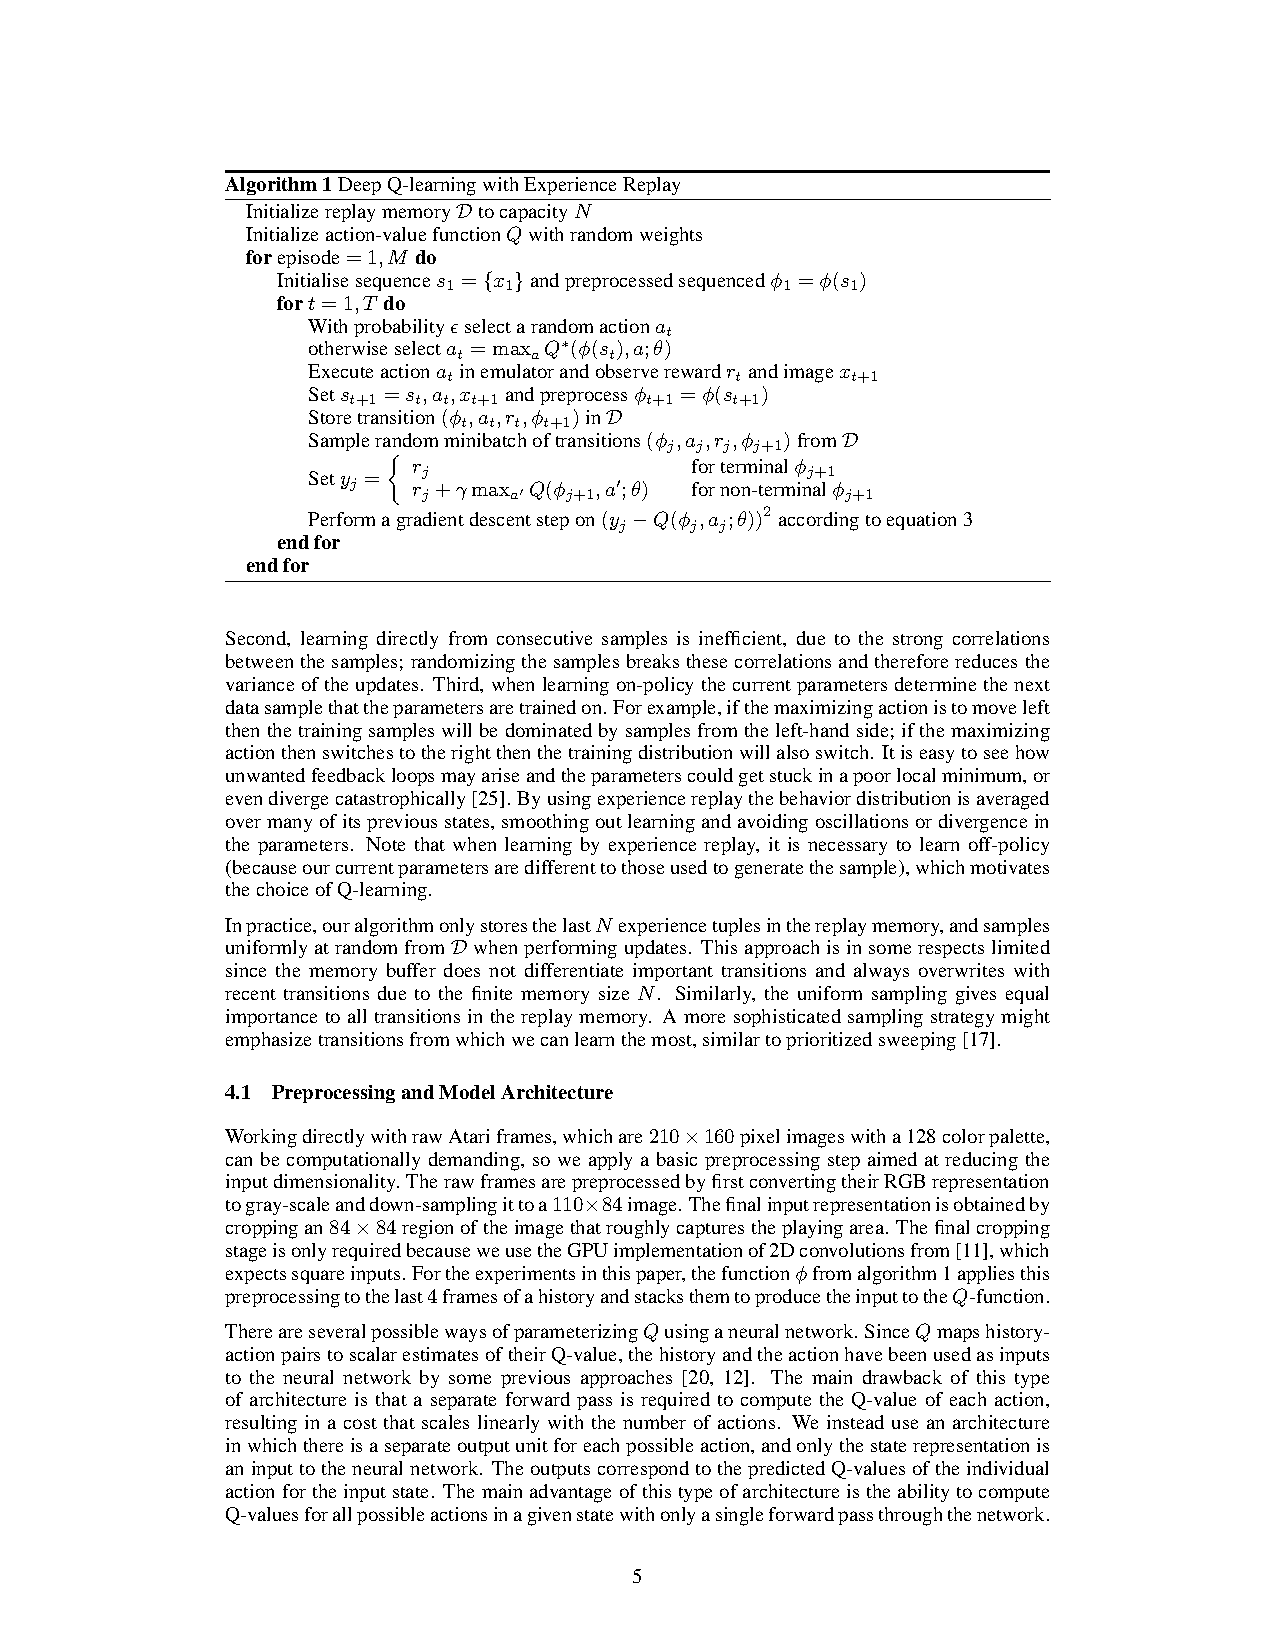
\includegraphics[width=0.99\textwidth, trim={60 500 60 60}, clip]{figures/Experience_Replay.pdf}};
    \begin{scope}[x={(image.south east)},y={(image.north west)}]
        \draw[blue,thick,rounded corners] (0.6,0.41) rectangle (0.1,0.51); % Draw the blue box
        % \draw[->, ultra thick, blue] (0.6,0.72) -- (0.70,0.72); % Draw the blue arrow
        \node[draw, text width=3cm, align=center, blue, font=\footnotesize] at (0.85,0.50) {Take the action ($a_t$), \\
and observe the reward $r_t$\\
    and next state $s_{t+1}$}; % Add the blue text box
    \end{scope}
\end{tikzpicture}
\end{center}
\end{frame}

%---------------------------------------------
\begin{frame}{Experience Replay Algorithm}
\begin{center}
\begin{tikzpicture}
    \node[anchor=south west,inner sep=0] (image) at (0,0) {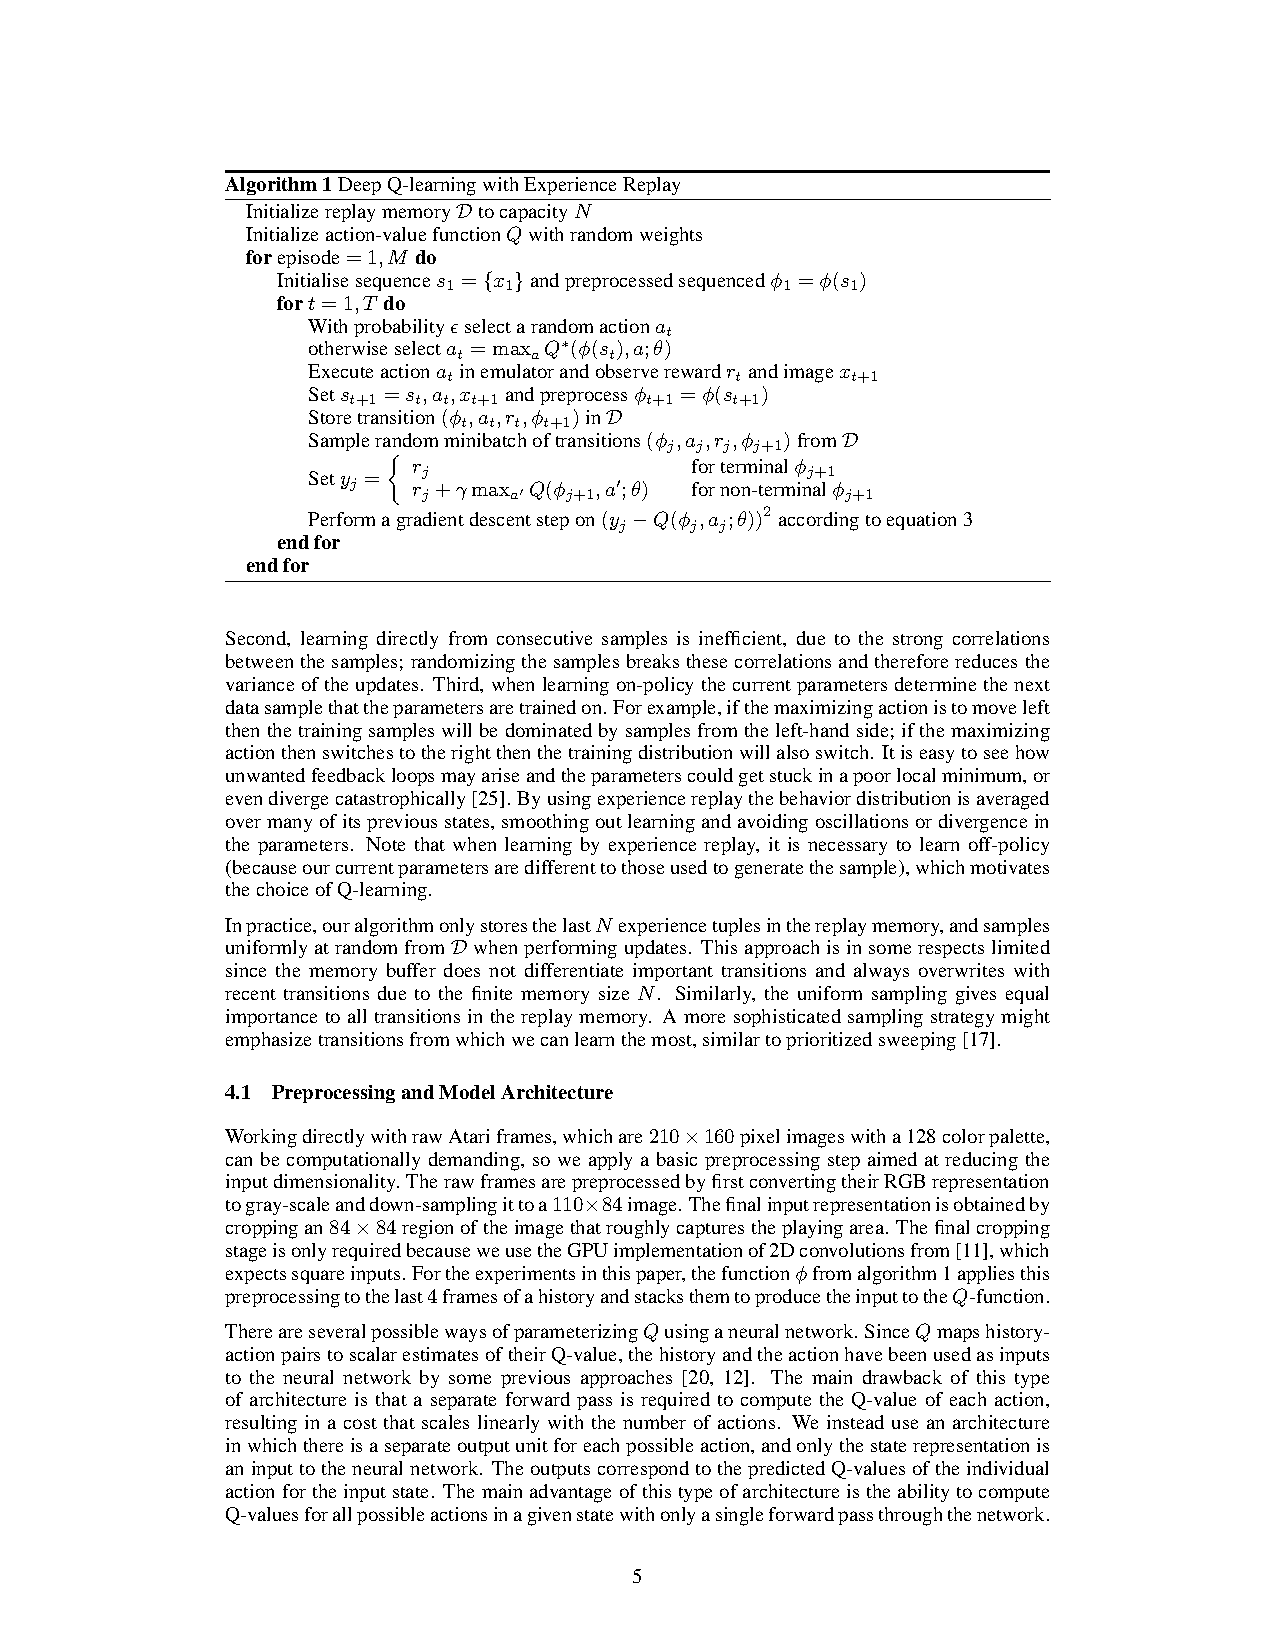
\includegraphics[width=0.99\textwidth, trim={60 500 60 60}, clip]{figures/Experience_Replay.pdf}};
    \begin{scope}[x={(image.south east)},y={(image.north west)}]
        \draw[blue,thick,rounded corners] (0.6,0.37) rectangle (0.1,0.43); % Draw the blue box
        % \draw[->, ultra thick, blue] (0.6,0.72) -- (0.70,0.72); % Draw the blue arrow
        \node[draw, text width=3cm, align=center, blue, font=\footnotesize] at (0.85,0.50) {Store transition in replay memory}; % Add the blue text box
    \end{scope}
\end{tikzpicture}
\end{center}
\end{frame}

%---------------------------------------------
\begin{frame}{Experience Replay Algorithm}
\begin{center}
\begin{tikzpicture}
    \node[anchor=south west,inner sep=0] (image) at (0,0) {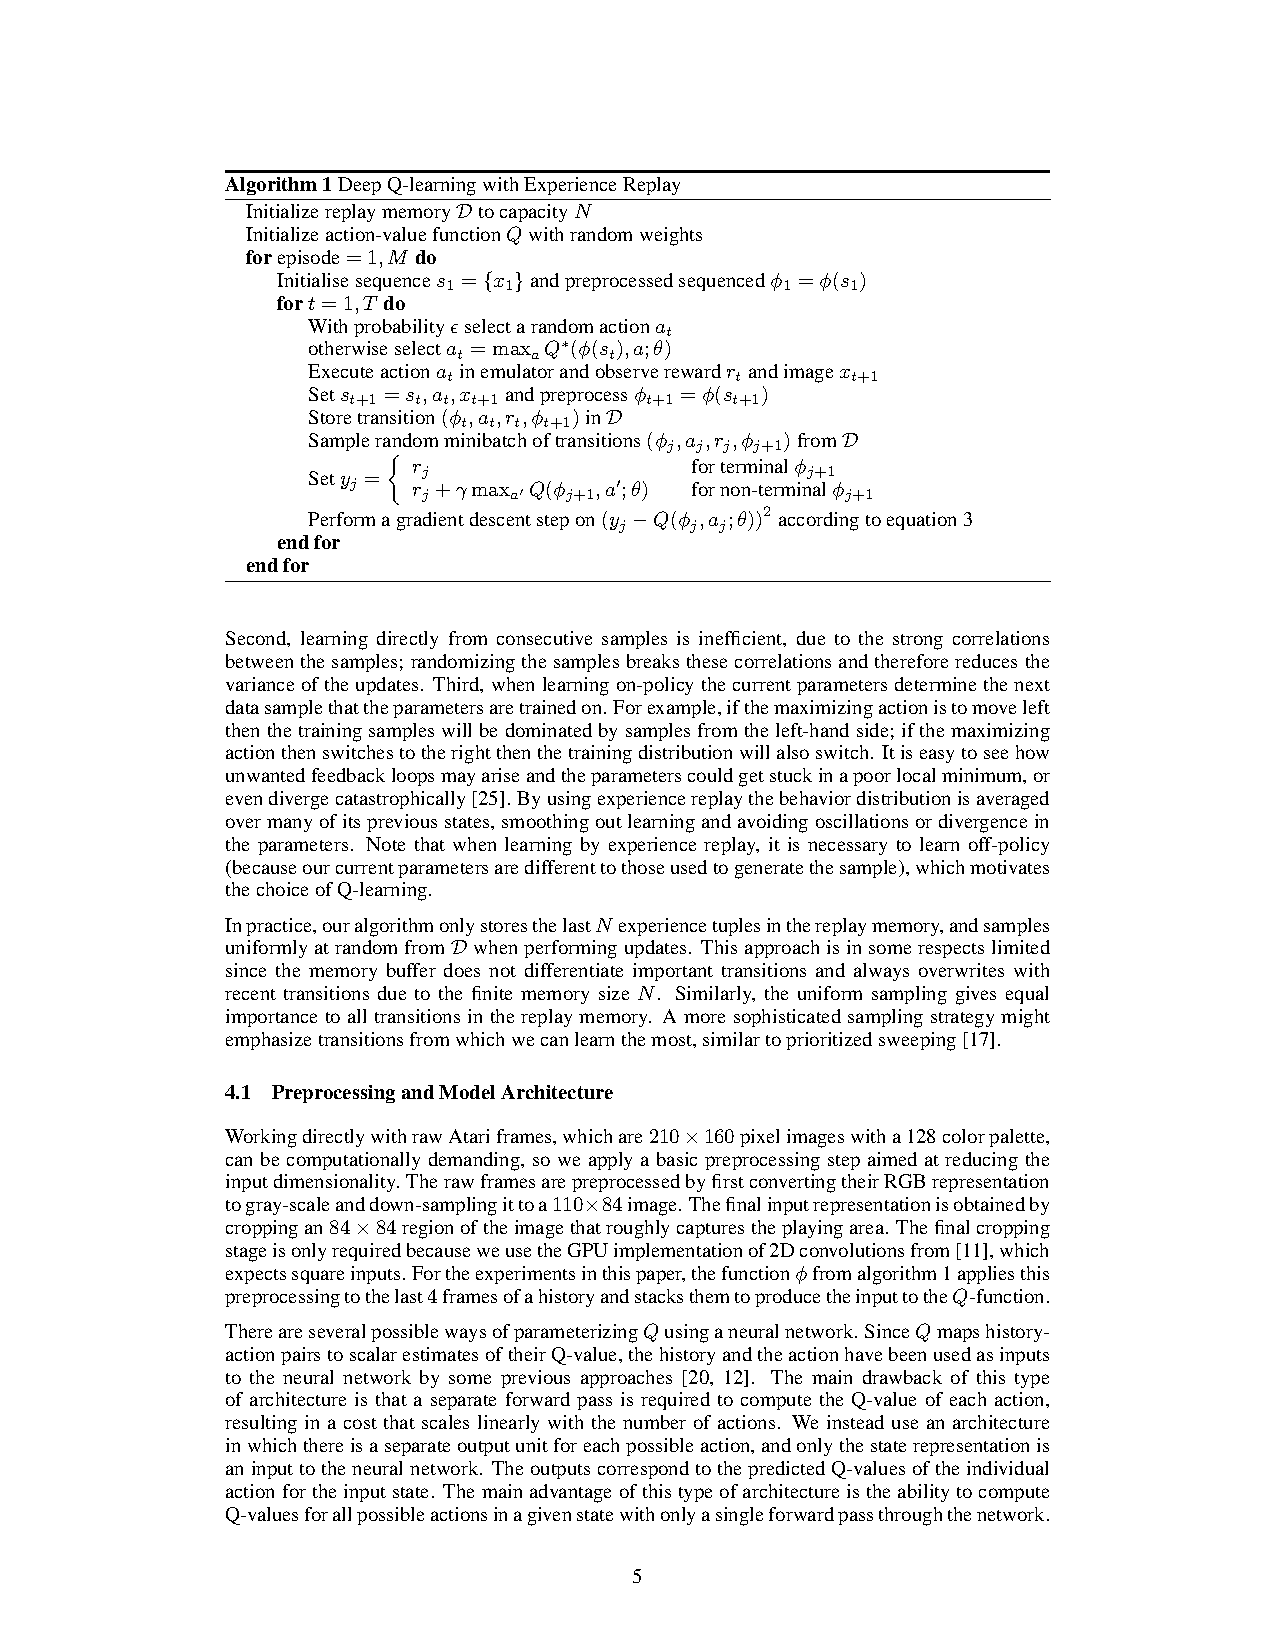
\includegraphics[width=0.99\textwidth, trim={60 500 60 60}, clip]{figures/Experience_Replay.pdf}};
    \begin{scope}[x={(image.south east)},y={(image.north west)}]
        \draw[blue,thick,rounded corners] (0.6,0.16) rectangle (0.1,0.37); % Draw the blue box
        % \draw[->, ultra thick, blue] (0.6,0.72) -- (0.70,0.72); % Draw the blue arrow
        \node[draw, text width=3cm, align=center, blue, font=\footnotesize] at (0.85,0.50) {Experience Replay:
Sample a random
minibatch of transitions
from replay memory
and perform a gradient
descent step}; % Add the blue text box
    \end{scope}
\end{tikzpicture}
\end{center}
\end{frame}   

\begin{frame}{}
\begin{center}
    \Large 
    Let's do some coding
\end{center}
\end{frame}

% \begin{frame}[fragile]{Creating Grid World}

%     \begin{block}{Imagine a $4 \times 4$ grid with:}
%         \begin{itemize}
%             \item \textbf{Goal} at $(3,3)$ giving $+1$ reward
%             \item \textbf{Penalty} at $(1,1)$ giving $-1$ reward
%             \item \textbf{4 possible moves:} Up, Right, Down, Left
%         \end{itemize}
%     \end{block}
% \end{frame}

%---------------------------------------------
\begin{frame}{Problem with Q-learning}
\begin{gradblock}{Problem with Q-learning}
    \begin{itemize}
        \item Q-learning can model scenarios where the action space is discrete and small.
        \item The formulation we saw can't handle continuous action spaces.
        \item Policy is deterministically calculated by maximizing the reward $\to$ cannot learn stochastic policy.
\end{itemize}
\end{gradblock}
\end{frame}

% Add more frames as needed 
%---------------------------------------------
\begin{frame}{Problem with Q-learning}
\begin{gradblock}{Problem with Q-learning}
    The Q-function can be very complicated!
    
    \vspace{10pt}
    \textbf{Example:} a robot grasping an object has a very high-dimensional state $\to$ hard
to learn the exact value of every (state, action) pair.

\vspace{10pt}
But the policy can be much simpler: simply close your hand.

Can we learn a policy directly, e.g. finding the best policy from a collection of policies?

\end{gradblock}
\end{frame}

% Add more frames as needed 
%---------------------------------------------
\begin{frame}{Formulating Policy Gradients}

    \begin{center}
        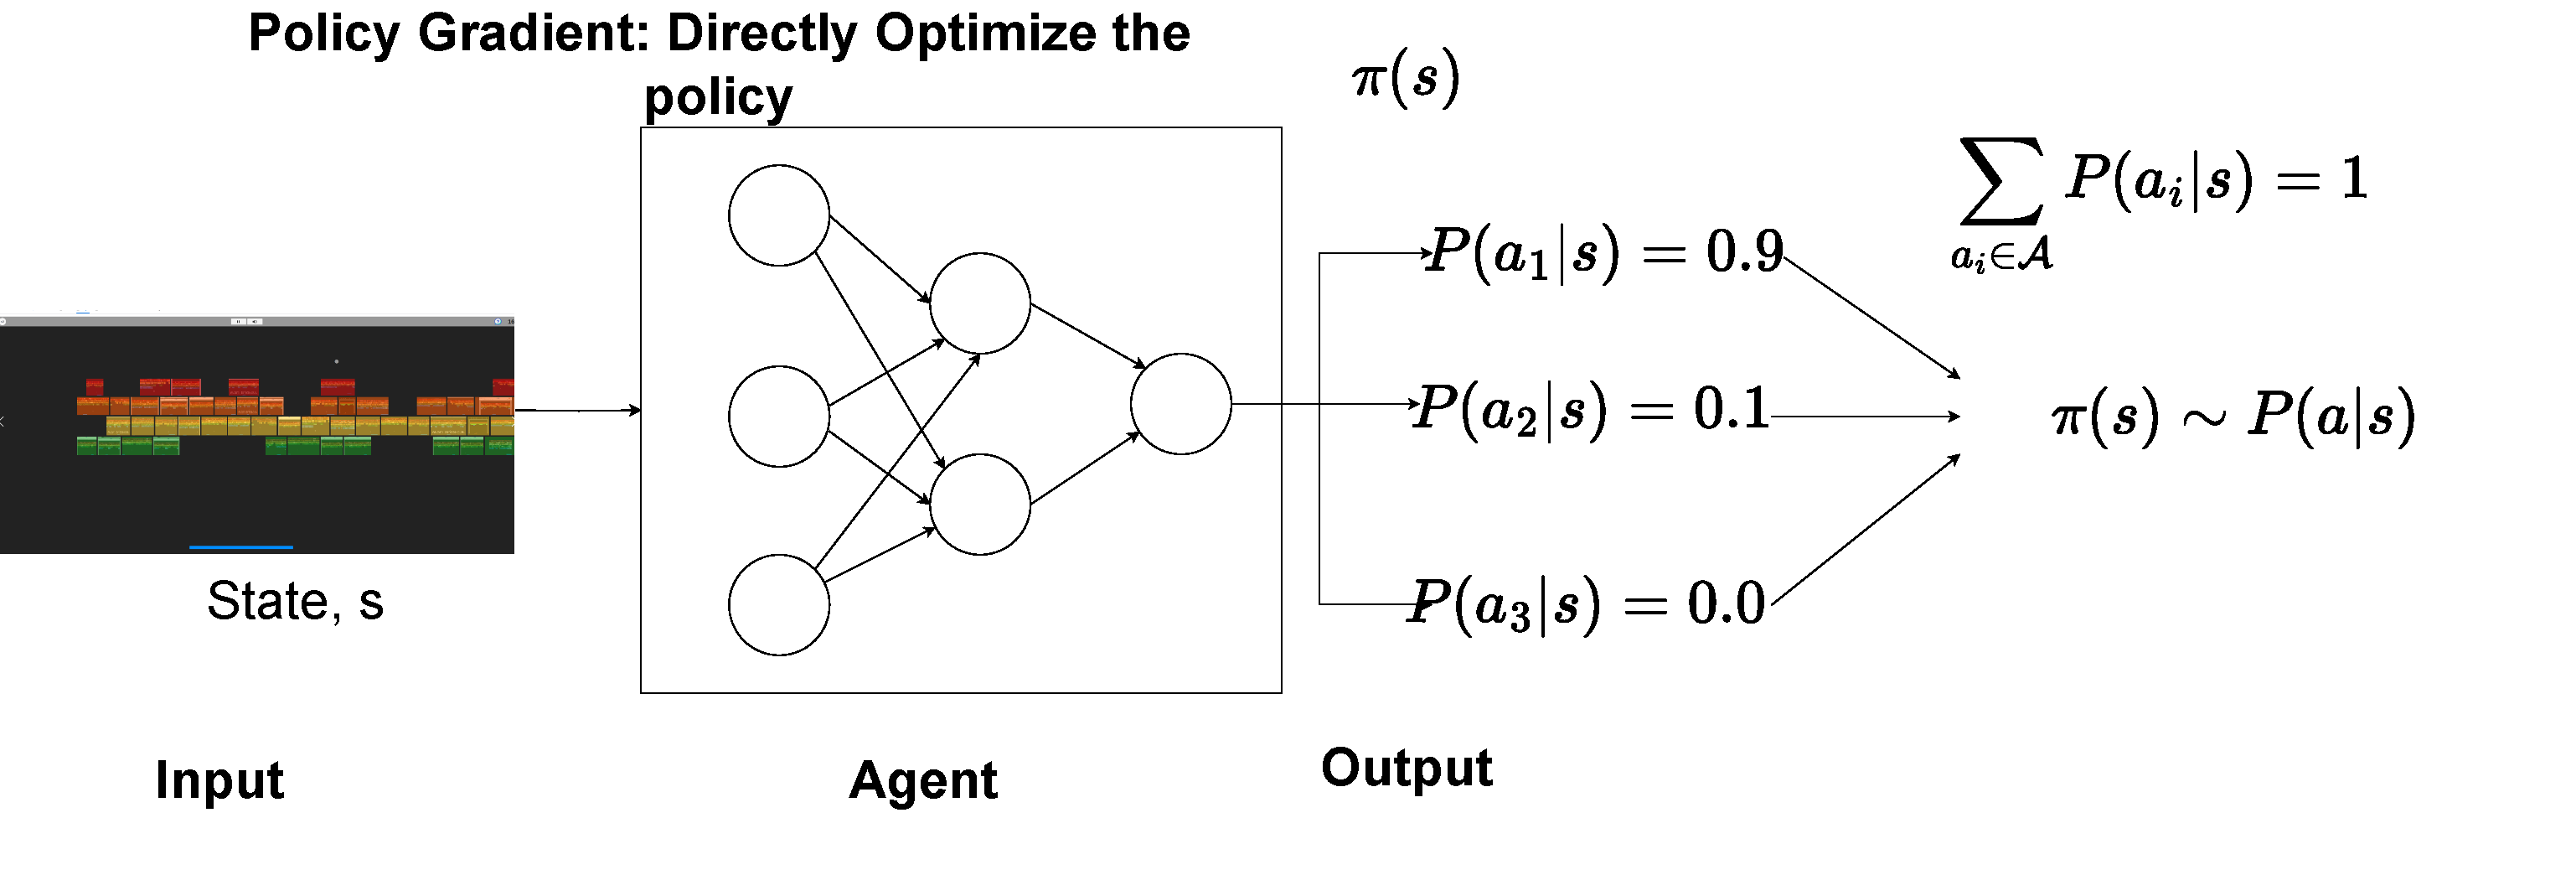
\includegraphics[width=0.85\textwidth]{figures/PolicyGradient_1.pdf}
    \end{center}

Sample from $\pi(s)$, explore the environment, and obtain some stochasticity.
\end{frame}

%---------------------------------------------
\begin{frame}{Formulating Policy Gradients}

    \begin{center}
        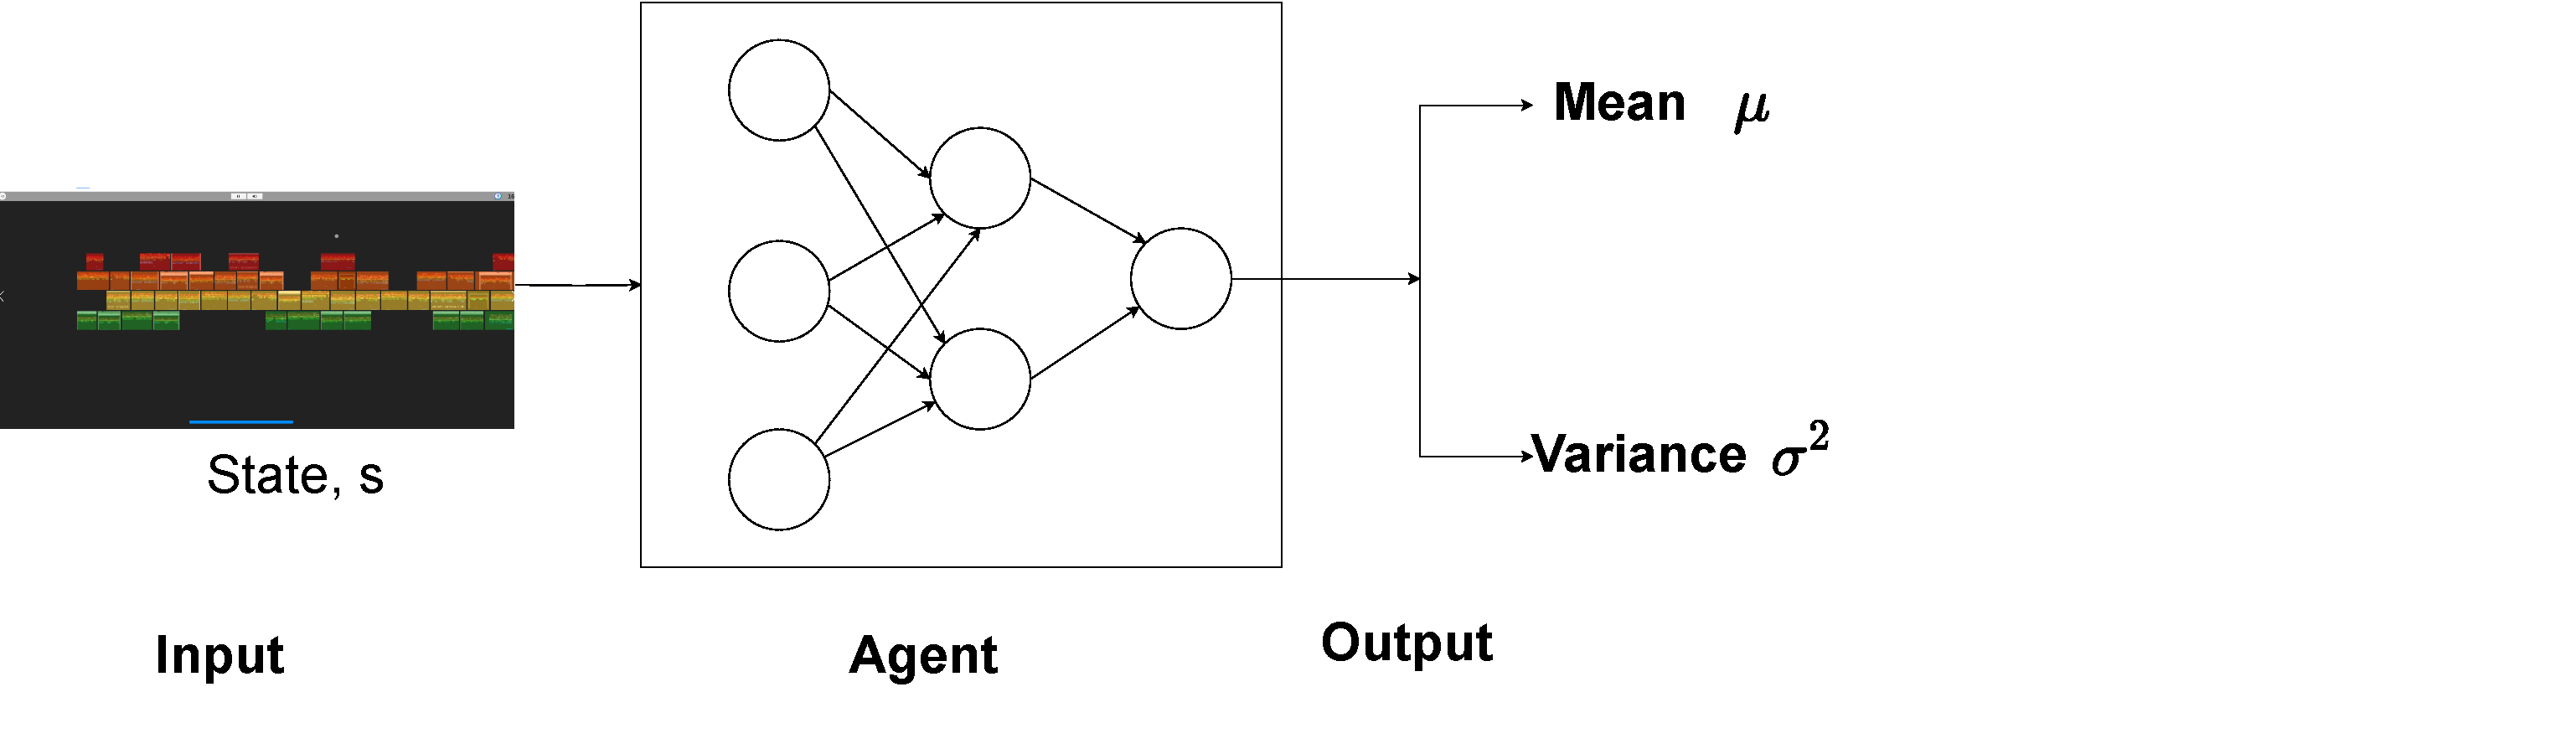
\includegraphics[width=0.85\textwidth]{figures/PolicyGradient_2.pdf} 
        $P(a|s)\sim \Ncal (\mu, \sigma^2)$.
    \end{center}

\url{https://link.springer.com/article/10.1007/BF00992696}

\end{frame}

%---------------------------------------------
\begin{frame}{Example: Self-driving Cars}
\begin{columns}[c]
    \column{.60\textwidth} 
\begin{itemize}
    \item \textbf{Agent: } vehicle
    \item \textbf{State: } comes from sensor measurements: camera, Lidar, etc.
    \item \textbf{Action: } steering wheel angle
    \item \textbf{Reward: } distance traveled
\end{itemize}
\column{.40\textwidth} 
    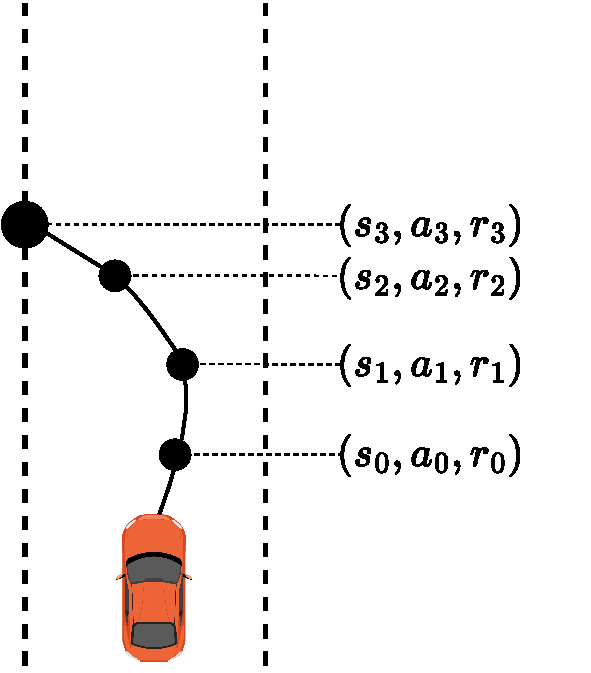
\includegraphics[width=0.99\textwidth]{figures/car_training.pdf} 
\end{columns}
\end{frame}

%---------------------------------------------
\begin{frame}{Training Policy Gradients}
\begin{columns}[c]
    \column{.60\textwidth} 
    \textbf{Training Algorithm}
    \begin{itemize}
        \item Initialize the agent
        \item Run a policy until termination
        \item Record all states, actions, rewards
        \item Decrease the probability of actions that resulted in low reward.
        \item Increase probability of actions that lead to high rewards
    \end{itemize}
\column{.40\textwidth} 
    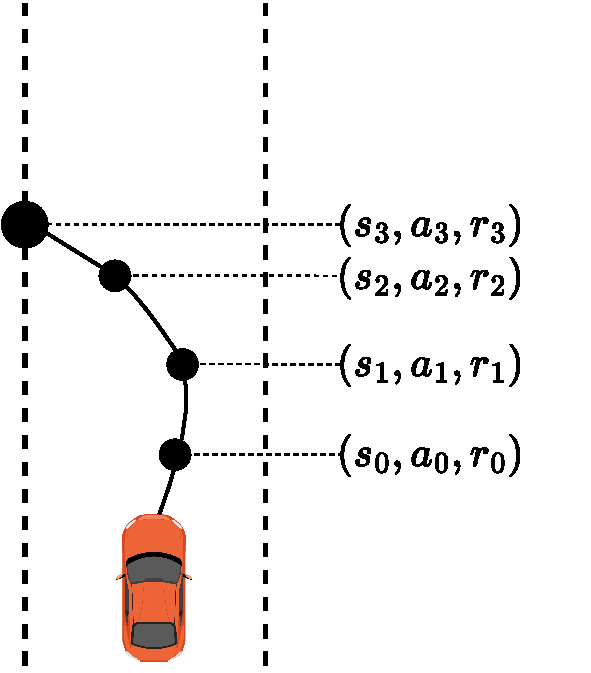
\includegraphics[width=0.99\textwidth]{figures/car_training.pdf} 
\end{columns}


\end{frame}

%-------------------------------------
\begin{frame}{REINFORCE Algorithm for Policy Gradients}
    \begin{center}
        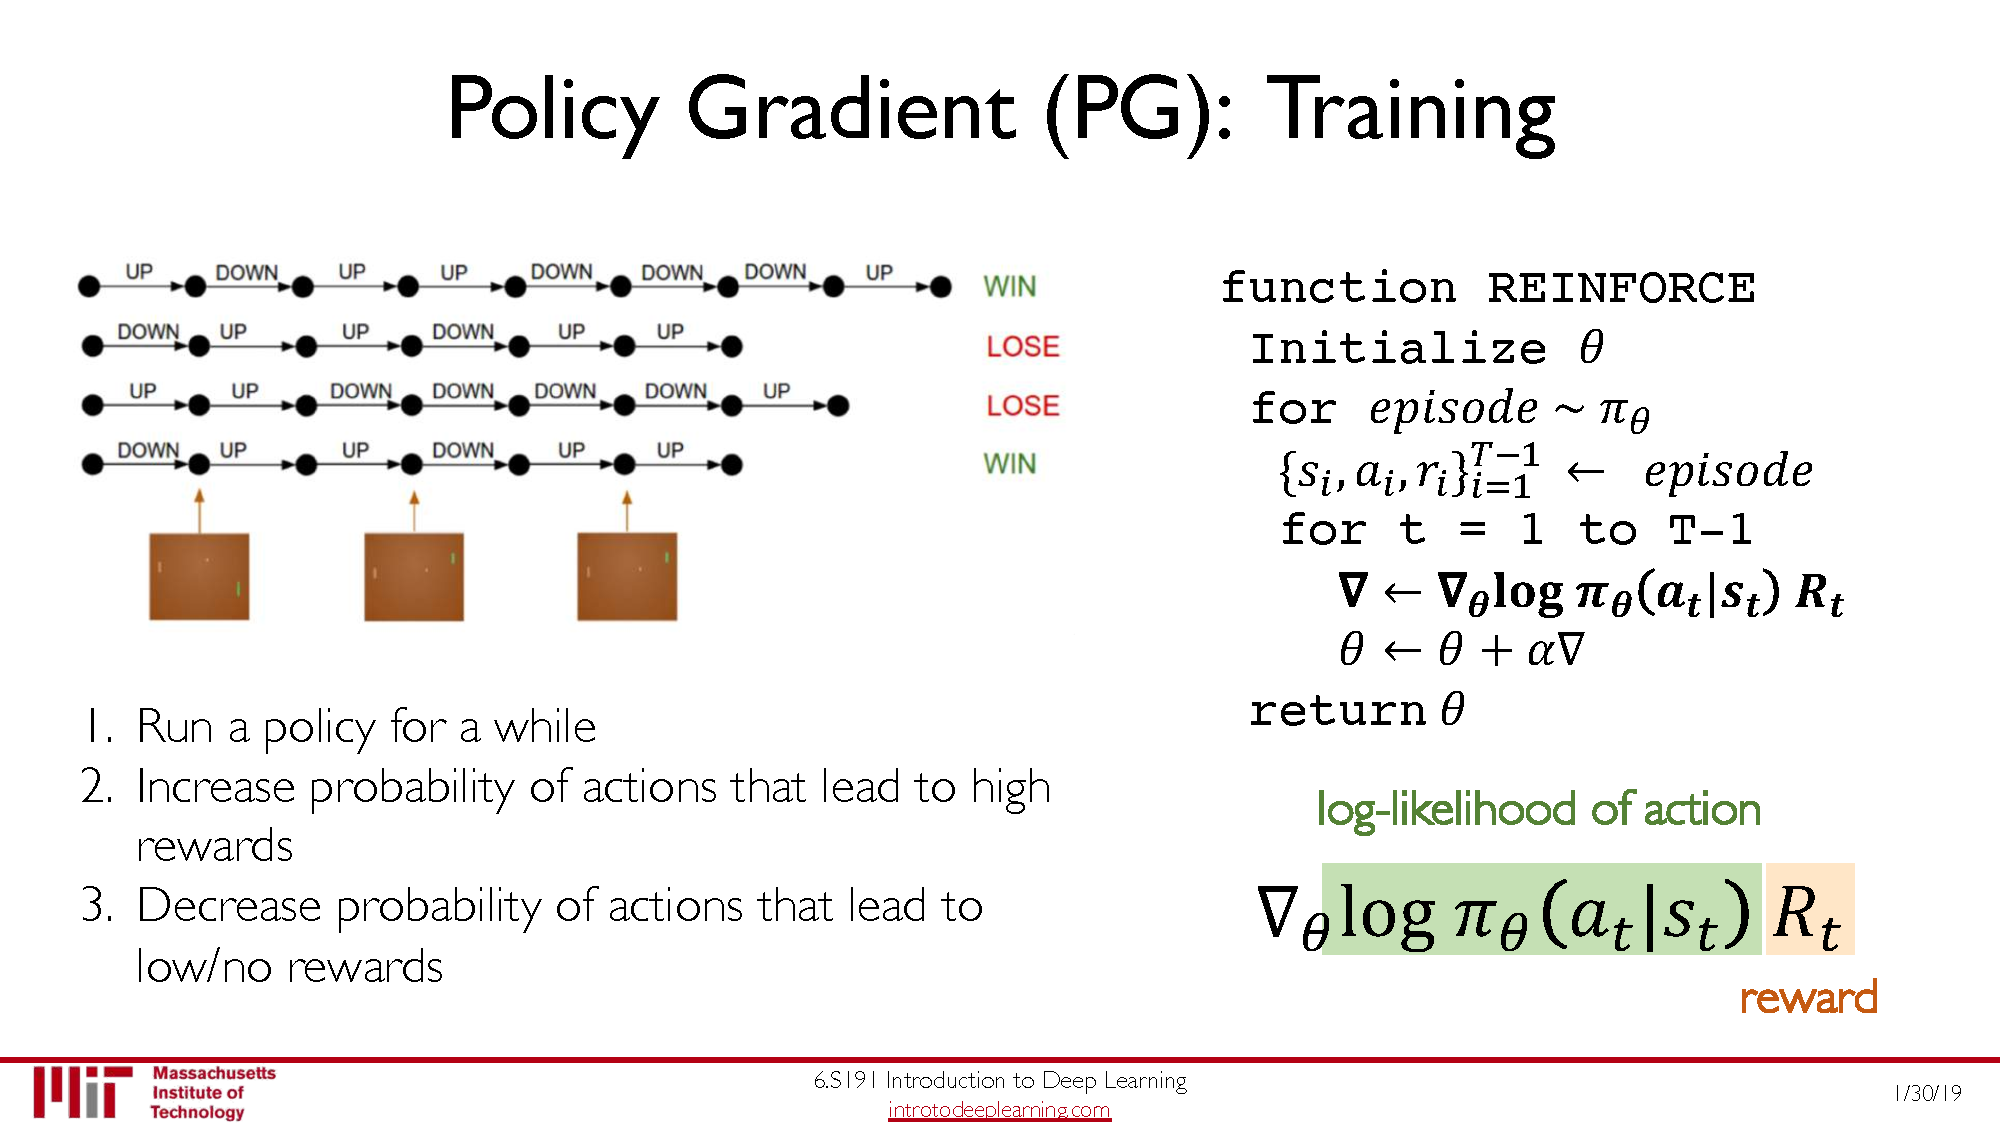
\includegraphics[width=0.39\textwidth, trim={540 50 6 100}, clip]{figures/Reinforce.pdf}
    \end{center}
\end{frame}

%------------------------------------------------

\begin{frame}
    \Large {\centerline{\textbf{Code Demo of Snake RL Game}}}

    \begin{center}
        \url{https://github.com/rahulbhadani/CPE490_590_Sp2025/tree/master/Code/RL_Snake}
    \end{center}

    Run \texttt{python agent.py} to train aan RL agent.

    Run \texttt{python snake\_game\_original.py} and use arrow keys to play game by yourself.

\end{frame}

%------------------------------------------------
\begin{frame}{The idea behind using Q-learning in Snake Game}
    \begin{tblock}{}
        Originally, Q-learning would maintain a table of values  that gives us the expected future reward for taking action \texttt{a} in state \texttt{s}
        \begin{multiequation}
            Q(s,a) = Q(s,a) + \eta[r + \gamma max(Q(s',a')) - Q(s,a)]
        \end{multiequation}
        where $\eta$ is the learning rate. $max(Q(s',a'))$ is the maximum expected future reward from the new state.
        
    \end{tblock}
\end{frame}

\begin{frame}{An Example $4\times 5$ Grid}
    \small
    \begin{center}
        \begin{tabular}{c c}
            \multicolumn{1}{c}{Grid} & \multicolumn{1}{c}{Reward} \\
            \begin{tabular}{|c|c|c|c|c|}
            \hline
            (0,0) & (0,1) & (0,2) & (0,3) & (0,4) \\
            \hline
            (1,0) & (1,1) & (1,2) & (1,3) & (1,4) \\
            \hline
            (2,0) & (2,1) & (2,2) & (2,3)  & (2, 4)\\
            \hline
            (3,0) & (3,1) & (3,2) & (3,3)  & (3, 4)\\
            \hline
        \end{tabular}
        &
        \begin{tabular}{|c|c|c|c|c|}
        \hline
        -1 & -1 & -1 & -1 & +100 \\
        \hline
        -1 & -100 & -1 & -1 & -1\\ % Assuming the black square is a wall
        \hline
        -1 & -1 & -1 & -1  & -1\\
        \hline
        -1 & -1 & -1 & -1 & +100 \\
        \hline
        \end{tabular}
        \end{tabular}

        \begin{tabular}{c}

        \multicolumn{1}{c}{Movement} \\

        \begin{tabular}{|c|c|c|c|c|}
            \hline
            \perparrows{0.5}{0.5}{0.5pt}{1.5mm}{blue}{red} &  \perparrows{0.5}{0.5}{0.5pt}{1.5mm}{blue}{red} &  \perparrows{0.5}{0.5}{0.5pt}{1.5mm}{blue}{red} & \perparrows{0.5}{0.5}{0.5pt}{1.5mm}{blue}{red}  & \cellcolor{red!25} \\ % Using color requires \usepackage{colortbl}, \usepackage{xcolor}
            \hline
            \perparrows{0.5}{0.5}{0.5pt}{1.5mm}{blue}{red} &  \perparrows{0.5}{0.5}{0.5pt}{1.5mm}{blue}{red} & \cellcolor{black}  &  \perparrows{0.5}{0.5}{0.5pt}{1.5mm}{blue}{red} &  \perparrows{0.5}{0.5}{0.5pt}{1.5mm}{blue}{red}  \\ 
            \hline
            \perparrows{0.5}{0.5}{0.5pt}{1.5mm}{blue}{red} &  \perparrows{0.5}{0.5}{0.5pt}{1.5mm}{blue}{red} &  \perparrows{0.5}{0.5}{0.5pt}{1.5mm}{blue}{red} &  \perparrows{0.5}{0.5}{0.5pt}{1.5mm}{blue}{red} & \perparrows{0.5}{0.5}{0.5pt}{1.5mm}{blue}{red}\\ % Assuming blue represents start/current
            \hline
            \perparrows{0.5}{0.5}{0.5pt}{1.5mm}{blue}{red} &  \perparrows{0.5}{0.5}{0.5pt}{1.5mm}{blue}{red}  &  \perparrows{0.5}{0.5}{0.5pt}{1.5mm}{blue}{red} & \perparrows{0.5}{0.5}{0.5pt}{1.5mm}{blue}{red} & \cellcolor{red!25}  \\ % Assuming red represents goal/terminal
            \hline
        \end{tabular}
    \end{tabular}

        When the movement causes to hit the wall, state doesn't change.

        Consider $\eta = 0.5$, $\gamma = 0.9$.
    \end{center}
\end{frame}


\begin{frame}{An Example $4\times 5$ Grid}
\begin{center}
    Initial Q values to zero. $Q(s, a) = 0.0$ for all $s$ and $a$. 
    
    \vspace{0.5cm}

    \textbf{Episode 1}
    
    \vspace{0.5cm}

    \begin{tabular}{c}
        \multicolumn{1}{c}{Start at $(2, 1)$.} \\
        \begin{tabular}{|c|c|c|c|c|}
        \hline
        ~~ &  ~~ &  ~~  & ~~ & \cellcolor{red!25} \\ % Using color requires \usepackage{colortbl}, \usepackage{xcolor}
        \hline
        ~~ & ~~ & \cellcolor{black}  &  ~~ &  ~~  \\ 
        \hline
        ~~ & \footnotesize \faStar $\to$ &  ~~ & ~~ & ~~ \\ % Assuming blue represents start/current
        \hline
        ~~ & ~~  &  ~~ & ~~ & \cellcolor{red!25}  \\ % Assuming red represents goal/terminal
        \hline
        \end{tabular}
    \end{tabular}

    Randomly pick an action: Say Right ($a = \text{Right}$). \\
    Transition: $(2,1) \rightarrow (2,2)$. \\
    Reward received: $r = -1$. \\
    New state: $s' = (2,2)$.

\end{center}
\end{frame}

\begin{frame}{An Example $4\times 5$ Grid: Q-value Calculation}

    \begin{center}
        \begin{multiequation}
            Q((2,1), \text{Right}) & = Q((2,1), \text{Right}) + \eta [r + \gamma \max_{a'} Q(s'=(2,2), a') - Q((2,1), \text{Right})] \\
            & = 0 + 0.5 [-1 + 0.9 \max_{a'} Q((2,2), a') - 0] \\
            & = 0 + 0.5 [-1 + 0.9 \times 0 - 0] \quad \text{(Since all initial Q values are 0)} \\
            & =  0.5 [-1] \\
            & = -0.5
        \end{multiequation}
    \end{center}
\end{frame}

\begin{frame}{An Example $4\times 5$ Grid: Continue}
    \begin{center}
        At $(2,2)$, 
        
        \vspace{0.5cm}
    
        \textbf{Episode 1}
        
        \vspace{0.5cm}
    
        \begin{tabular}{c}
            \multicolumn{1}{c}{Start at $(2, 1)$.} \\
            \begin{tabular}{|c|c|c|c|c|}
            \hline
            ~~ &  ~~ &  ~~  & ~~ & \cellcolor{red!25} \\ % Using color requires \usepackage{colortbl}, \usepackage{xcolor}
            \hline
            ~~ & ~~ & \cellcolor{black}  &  ~~ &  ~~  \\ 
            \hline
            ~~ &  &  \footnotesize \faStar $\to$ & ~~ & ~~ \\ % Assuming blue represents start/current
            \hline
            ~~ & ~~  &  ~~ & ~~ & \cellcolor{red!25}  \\ % Assuming red represents goal/terminal
            \hline
            \end{tabular}
        \end{tabular}
    
        Randomly pick an action: Say Right ($a = \text{Right}$). \\
        Transition: $(2,2) \rightarrow (2,3)$. \\
        Reward received: $r = -1$. \\
        New state: $s' = (2,3)$.
    
    \end{center}
    \end{frame}

    \begin{frame}{An Example $4\times 5$ Grid: Q-value Calculation}

        \begin{center}
            \begin{multiequation}
                Q((2,2), \text{Right}) & = Q((2,2), \text{Right}) + \eta [r + \gamma \max_{a'} Q(s'=(2,3), a') - Q((2,2), \text{Right})] \\
                & = 0 + 0.5 [-1 + 0.9 \max_{a'} Q((2,3), a') - 0] \\
                & = 0 + 0.5 [-1 + 0.9 \times 0 - 0] \quad \text{(Since all initial Q values are 0)} \\
                & =  0.5 [-1] \\
                & = -0.5
            \end{multiequation}
        \end{center}
    \end{frame}

    \begin{frame}{An Example $4\times 5$ Grid: Continue}
        \begin{center}
            At $(2,3)$, 
            
            \vspace{0.5cm}
        
            \textbf{Episode 1}
            
            \vspace{0.5cm}
        
            \begin{tabular}{c}
                \multicolumn{1}{c}{Start at $(2, 1)$.} \\
                \begin{tabular}{|c|c|c|c|c|}
                \hline
                ~~ &  ~~ &  ~~  & ~~ & \cellcolor{red!25} \\ % Using color requires \usepackage{colortbl}, \usepackage{xcolor}
                \hline
                ~~ & ~~ & \cellcolor{black}  &  ~~ &  ~~  \\ 
                \hline
                ~~ &  & ~~ & \footnotesize \faStar $\to$ & ~~ \\ % Assuming blue represents start/current
                \hline
                ~~ & ~~  &  ~~ & ~~ & \cellcolor{red!25}  \\ % Assuming red represents goal/terminal
                \hline
                \end{tabular}
            \end{tabular}
        
            Randomly pick an action: Say Right ($a = \text{Right}$). \\
            Transition: $(2,3) \rightarrow (2,4)$. \\
            Reward received: $r = -1$. \\
            New state: $s' = (2,4)$, and $Q((2,3), \text{Right})  = -0.5$
        
        \end{center}
    \end{frame}

    \begin{frame}{An Example $4\times 5$ Grid: Continue}
        \begin{center}
            At $(2,4)$, 
            
            \vspace{0.5cm}
        
            \textbf{Episode 1}
            
            \vspace{0.5cm}
        
            \begin{tabular}{c}
                \multicolumn{1}{c}{Start at $(2, 1)$.} \\
                \begin{tabular}{|c|c|c|c|c|}
                \hline
                ~~ &  ~~ &  ~~  & ~~ & \cellcolor{red!25} \\ % Using color requires \usepackage{colortbl}, \usepackage{xcolor}
                \hline
                ~~ & ~~ & \cellcolor{black}  &  ~~ &  ~~  \\ 
                \hline
                ~~ &  & ~~ & ~~ & \footnotesize \faStar $\downarrow$ \\ % Assuming blue represents start/current
                \hline
                ~~ & ~~  &  ~~ & ~~ & \cellcolor{red!25}  \\ % Assuming red represents goal/terminal
                \hline
                \end{tabular}
            \end{tabular}
        
            Randomly pick an action: Say Down ($a = \text{Right}$). \\
            Transition: $(2,4) \rightarrow (3,4)$. \\
            Reward received: $r = +100$. \\
            New state: $s' = (3,4)$, and $Q((2,3), \text{Right})  = +50$\\
            
            \textbf{We reach our goal, episode 1 ends.}
            
        \end{center}
    \end{frame}

    \begin{frame}{An Example $4\times 5$ Grid: Episode 2}
        \Large 
        \begin{itemize}
            \item Episode 2 uses updated $Q(s,a)$ values from Episode 1.
            \item How does action probability change?
            \item \begin{itemize}
                \item Epsilon-greedy Action Selection
                \item Softmax (Boltzmann) Action Selection
            \end{itemize}
        \end{itemize}
    \end{frame}

    \begin{frame}{The Case of Exploitation vs Exploration}
        \begin{tblock}{Exploration}
            \begin{itemize}
                \item Trying out different actions to discover more about the environment and potential rewards.
                \item Analogous to randomly exploring the levers of slot machines to see which one gives the best payout.
            \end{itemize}
        \end{tblock}
    \end{frame}

    \begin{frame}{The Case of Exploitation vs Exploration}

        \begin{tblock}{Exploitation}
            \begin{itemize}
                \item Using the current knowledge to choose the action that is believed to yield the highest reward.
                \item Analogous to repeatedly playing the slot machine that has given the best payout so far.
            \end{itemize}
        \end{tblock}
        \textbf{Reference:} Deep Reinforcement Learning in Action By Alexander Zai, Brandon Brown 

    \end{frame}

    \begin{frame}{Epsilon-greedy Action Selection}

        \footnotesize

        After each episode, the agent learn something new. Hence, after episode 1, it has capability to exploit (based on what it learnt) in addition to explore. 

        \begin{tblock}{$\epsilon$-greedy Approach}
            \begin{itemize}
                \item With probability $1-\epsilon$, choose the best action (with highest Q value)
                \item With probability $\epsilon$, pick randomly among all actions
            \end{itemize}
        \end{tblock}
        
        Mathematically, 
        \begin{multiequation}
            \pi (a|s) = \begin{cases}
                1 - \epsilon + \cfrac{\epsilon}{|\Acal|}, \quad \text{~if~best~action}\\
                \cfrac{\epsilon}{|\Acal|}, \quad \text{otherwise}
            \end{cases}
        \end{multiequation}
        \textbf{Reference:} Section 5.4 Reinforcement Learning An Introduction 2nd ed, Richard S. Sutton and Andrew G. Barto

        
    \end{frame}
    % \begin{frame}
%     \huge{\centerline{\textbf{TorchRL}}}
% \end{frame}

\begin{frame}{Actor-Critic Algorithm: Motivation}
The algorithms we saw above are of two types:
\begin{itemize}
    \item \textbf{Actor-only:} methods work with a parameterized family of policies (policy gradients).  The gradient of the performance, with respect to the actor parameters, is directly estimated by simulation, and the parameters are updated in the direction of improvement.
    \item \textbf{Critic-only:} rely exclusively on value function approximation and
aim at learning an approximate solution to the Bellman equation, which will then hopefully prescribe a near-optimal policy (Q-learning).
\end{itemize}

    \begin{center}
    \color{Emerald}
        {\Large Actor-critic combines the strong points of actor-only and critic-only methods.}
    \end{center}
\end{frame}



%------------------------------------------------
\begin{frame}{Actor-critic Algorithms}
\begin{itemize}
    \item Estimate the policy, estimate the value function.
    \item Critic-only methods estimate the value function, policy is implicit. 
    \item Actor-only methods estimate the policy  and we don't work with value functions
\end{itemize}

\vspace{10pt}
\begin{center}\color{SlateBlue}
    You can consider that this algorithm has two parts: actor and critic. The actor decides which action should be taken and the critic informs the actor how good the action is and how it should adjust. 

    \vspace{10pt}
    \color{Red}
    This type of architecture also appears in GAN (Generative Adversarial Network) where `discriminator' and `generator' play games.
\end{center}    
\end{frame}


%------------------------------------------------
\begin{frame}{How does Actor-critic Algorithm works}
\begin{itemize}
    \item The actor decides which action to take, and the critic tells the actor how good its action was and how it should adjust
\item Also alleviates the task of the critic as it only has to learn the values of (state, action) pairs generated by the policy
\item Can also incorporate Q-learning tricks e.g. experience replay
\end{itemize}
\end{frame}
%------------------------------------------------

%------------------------------------------------
\begin{frame}{How to define how better the action was?}
\begin{center}
    {
    \Large How should we quantify how much an
action was better than expected?
    }
\end{center}
\begin{tblock}{Advantage function}
    $$
A^\pi (s, a) = Q^\pi(s, a) -  V^\pi(s)
$$
\end{tblock}

\end{frame}

%------------------------------------------------
\begin{frame}{Pseudo Code for Actor-Critic Algorithm}
    \begin{center}
        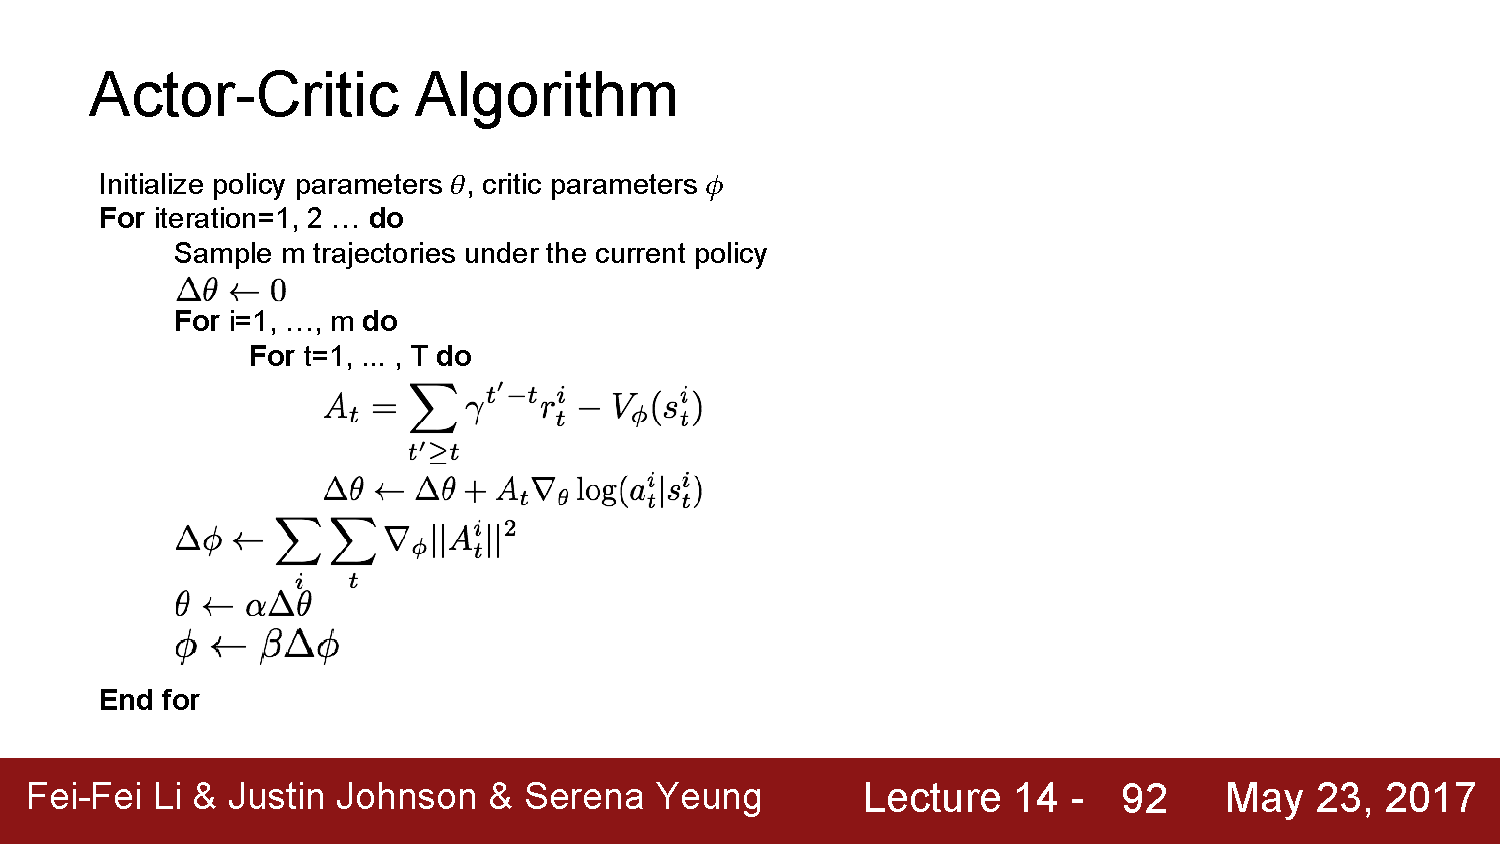
\includegraphics[width=0.99\textwidth, trim={5 45 6 80}, clip]{figures/actor_critic_algo.pdf}
    \end{center}
\end{frame}

\begin{frame}{Proximal Policy Optimization (PPO)}
    \begin{tblock}{}
        Improves  agent's training stability by avoiding policy updates that are too large. To do that, we use a ratio that indicates the difference between our current and old policy and clip this ratio to a specific range $[1-\epsilon,1+\epsilon]$.

    \end{tblock}
\end{frame}

\begin{frame}{The intuition behind PPO}
    The idea with Proximal Policy Optimization (PPO) is that we want to improve the training stability of the policy by limiting the change you make to the policy at each training epoch: we want to avoid having too large of a policy update.

    For two reasons:

    \begin{itemize}
        \item We know empirically that smaller policy updates during training are more likely to converge to an optimal solution.
        \item A too-big step in a policy update can result in falling “off the cliff” (getting a bad policy) and taking a long time or even having no possibility to recover.
    \end{itemize}
\end{frame}


\begin{frame}{PPO}
    To achieve this, we compare the new policy to the old one by computing the ratio of their action probabilities.

    This ratio tells us how much the policy has changed.

    To prevent the new policy from straying too far from the previous one, we clip this ratio within a fixed range $[1-\epsilon,1+\epsilon]$. 
    
    \begin{tblock}{}
        This clipping mechanism limits the size of policy updates, encouraging the new policy to stay "proximal" to the old policy and promoting more stable training.
    \end{tblock}


\end{frame}

\begin{frame}{ The Policy Objective Function}
    $$
    L^{PG}(\theta) = \Ebb_t[\overbrace{\log \pi_\theta(a_t|s_t)}^{\text{the log probability}\\\text{of taking action}} * \underbrace{A_t}_{\tiny\shortstack{\text{the advantage term (positive when the}\\\text{action is better than}\\\text{other possible actions at that state)}}}]
    $$
\footnotesize

    \text{The idea was that by taking a gradient ascent step on this function (equivalent to taking} \\
\text{gradient descent of the negative of this function), we would } \textbf{push our agent to} \\
\text{take actions that lead to higher rewards and avoid harmful actions.} \\
\text{However, the problem comes from the step size:} 
\begin{itemize}
    \item \text{Too small, } \textbf{the training process was too slow} \\
    \item \text{Too high, } \textbf{there was too much variability in the training}
\end{itemize}
\text{With PPO, the idea is to constrain our policy update with a new objective function} \\
\text{called the } \textit{Clipped surrogate objective function} \text{ that } \textbf{will constrain} \\
\text{the policy change in a small range using a clip.}

\end{frame}

\begin{frame}{Importance Sampling in PPO}
    \begin{tblock}{Probability Ratio}
        Instead of using the same policy, compare new and old policies using:
        \[
        r_t(\theta) = \frac{\pi_\theta(a_t | s_t)}{\pi_{\theta_{\text{old}}}(a_t | s_t)}
        \]
        where:
        \begin{itemize}
            \item $\theta_{\text{old}}$ are the parameters before the update.
            \item $r_t(\theta)$ measures how much the policy changed.
        \end{itemize}
    \end{tblock}
\end{frame}

\begin{frame}{Clipped Surrogate Objective Function}
    \begin{tblock}{Preventing Large Policy Changes}
        Define the clipped objective:
        \[
        L^{\text{CLIP}}(\theta) = \mathbb{E}_t \left[ \min\left( r_t(\theta) A_t, \, \text{clip}(r_t(\theta), 1 - \epsilon, 1 + \epsilon) A_t \right) \right]
        \]
        \vspace{0.2cm}
        \begin{itemize}
            \item If $r_t(\theta)$ changes too much, clipping ensures stable updates.
            \item $\epsilon$ is a hyperparameter (e.g., 0.2).
        \end{itemize}
    \end{tblock}
    \end{frame}

    \begin{frame}{Policy Update Rule}
        \begin{tblock}{Updating Policy Safely}
            After optimizing the clipped surrogate loss:
            \[
            \theta_{\text{old}} \leftarrow \theta
            \]
            \vspace{0.3cm}
            Repeat data collection and optimization to improve the policy iteratively.
        \end{tblock}
        \end{frame}

        \begin{frame}{Full PPO Objective}
            \begin{tblock}{Total Loss Function}
                PPO optimizes the combined objective:
                \[
                L(\theta) = L^{\text{CLIP}}(\theta) - c_1 L^{\text{VF}}(\theta) + c_2 S[\pi_\theta](s_t)
                \]
                where:
                \begin{itemize}
                    \item $L^{\text{CLIP}}(\theta)$: Clipped surrogate policy loss.
                    \item $L^{\text{VF}}(\theta)$: Value function loss (MSE between $V(s_t)$ and returns $R_t$).
                    \item $S[\pi_\theta](s_t)$: Entropy bonus to encourage exploration.
                    \item $c_1$, $c_2$: Coefficients to balance the terms.
                \end{itemize}
            \end{tblock}
            \end{frame}

            \begin{frame}{PPO: Example}
                \begin{tblock}{Environment Setup}
                \begin{itemize}
                    \item 1 state $s$, 2 actions: left and right.
                    \item Agent picks \textbf{right}, receives reward $r=1$.
                    \item Old policy: $\pi_{\theta_{\text{old}}}(\text{right}|s) = 0.4$
                    \item New policy: $\pi_\theta(\text{right}|s) = 0.6$
                    \item Estimated advantage: $\hat{A} = 2.0$
                \end{itemize}
                \end{tblock}
                
            \end{frame}

            \begin{frame}{PPO: Example}
                
                \begin{tblock}{Step-by-Step Computation}
                \begin{multiequation}
                r(\theta) &= \frac{0.6}{0.4} = 1.5 \\
                L_1 &= r(\theta) \cdot \hat{A} = 1.5 \cdot 2.0 = 3.0 \\
                r_{\text{clip}} &= \text{clip}(1.5, 0.8, 1.2) = 1.2 \\
                L_2 &= r_{\text{clip}} \cdot \hat{A} = 1.2 \cdot 2.0 = 2.4 \\
                L^{\text{CLIP}} &= \min(3.0, 2.4) = \boxed{2.4}
                \end{multiequation}
                \end{tblock}
                That’s the loss that would be used to update the policy network!
        \end{frame}

                
            % \begin{frame}{PPO Training Pipeline}
            %     \begin{center}
            %     \begin{tikzpicture}[node distance=2cm, auto, thick, align=center]
            %         % Nodes
            %         \node (collect) [rectangle, draw, rounded corners, fill=blue!10, minimum width=3cm, minimum height=1cm] {Collect Trajectories};
            %         \node (estimate) [rectangle, draw, rounded corners, fill=green!10, below of=collect] {Estimate \\ Returns $\&$ Advantages};
            %         \node (optimize) [rectangle, draw, rounded corners, fill=yellow!20, below of=estimate] {Optimize \\ Clipped Surrogate Loss};
            %         \node (update) [rectangle, draw, rounded corners, fill=red!20, below of=optimize] {Update \\ Policy Parameters};
                
            %         % Arrows
            %         \draw[->] (collect) -- (estimate);
            %         \draw[->] (estimate) -- (optimize);
            %         \draw[->] (optimize) -- (update);
            %         \draw[->, dashed] (update.south) .. controls +(down:3cm) and +(right:1cm) .. (collect.east) node[midway, right] {Repeat};
            %     \end{tikzpicture}
            %     \end{center}
            %     \end{frame}

                
%------------------------------------------------
\begin{frame}
    \Huge{\centerline{\color{MediumBlue}\textbf{The End}}}
\end{frame}



\end{document}